% =====================================================================
%  PROOF STUDY SHEETS — un seul fichier
%  Page 1 : synthèse Knowledge Locality + Correctness of FedPopper
%  Page 2 : synthèse Popper centralisé
%  Puis : Part I (SLD / Knowledge Locality), Part II (FedPopper),
%         Part III (Popper centralisé), en détail.
%  Compilation : pdflatex fiches-preuves.tex   (deux fois)
%  Couleurs : modifier uniquement les \definecolor ci-dessous.
% =====================================================================
\documentclass[10pt]{article}
\usepackage[utf8]{inputenc}
\usepackage[T1]{fontenc}
\usepackage[scaled]{helvet}
\renewcommand{\familydefault}{\sfdefault}
\usepackage[a4paper,margin=7mm]{geometry}
\usepackage{xcolor}
\usepackage[most]{tcolorbox}
\usepackage{tikz}
\usetikzlibrary{shapes.geometric}
\usepackage{pifont}
\usepackage{enumitem}
\usepackage{array}
\usepackage{etoolbox}
\usepackage{needspace}
\usepackage{amsmath,amssymb}
\usepackage{multirow}
\pagestyle{empty}
\setlength{\parindent}{0pt}

% ---------- Couleurs ----------
\definecolor{marine}{HTML}{3F72B8}   % bleu
\definecolor{pastel}{HTML}{BFD6F6}   % bleu pastel
\definecolor{fond}{HTML}{F4F7FB}
\definecolor{encre}{HTML}{1F1F1F}
\definecolor{vert}{HTML}{22A55B}
\definecolor{rouge}{HTML}{DC2626}
\pagecolor{fond}
\color{encre}

% ---------- Styles pages de synthèse ----------
\newtcolorbox{bloc}[2][]{enhanced, colback=white, colframe=pastel,
  boxrule=0.9pt, arc=0pt, left=5pt, right=5pt, top=3pt, bottom=3pt,
  fontupper=\footnotesize\raggedright, #1,
  before upper={{\large\bfseries\textcolor{marine}{#2}}\par\vspace{2pt}}}
\newtcolorbox{astuce}{colback=pastel!75, colframe=pastel!75, arc=0pt,
  boxrule=0pt, left=4pt, right=4pt, top=2pt, bottom=2pt,
  fontupper=\footnotesize\raggedright}
\newcommand{\num}[1]{\textcolor{marine}{\textbf{#1.}}~}
\newcommand{\fl}{\tikz[baseline=-0.6ex]\draw[->,thick](0,0)--(0.4,0);}
\newcommand{\sous}[1]{\textcolor{marine}{\textbf{#1}}\par}
\setlist[itemize]{leftmargin=9pt, itemsep=0pt, topsep=1pt, parsep=0pt,
  label=\textbullet, before=\raggedright}
\newcolumntype{L}[1]{>{\raggedright\arraybackslash}p{#1}}

% Terme anglais (en gras) avec sa traduction française
\newcommand{\EN}[2]{\textbf{#1}\,{\scriptsize\textcolor{marine}{(#2)}}}

% ---------- Styles pages détaillées ----------
\newtcolorbox{dire}{enhanced, breakable, colback=pastel!25, colframe=marine,
  boxrule=0pt, leftrule=3pt, arc=0pt, left=8pt, right=6pt, top=4pt, bottom=4pt,
  fontupper=\small\itshape, before upper={{\upshape\bfseries\textcolor{marine}{FR}}\enspace}}
\newtcolorbox{direEN}{enhanced, breakable, colback=vert!6, colframe=vert,
  boxrule=0pt, leftrule=3pt, arc=0pt, left=8pt, right=6pt, top=4pt, bottom=4pt,
  fontupper=\small\itshape, before upper={{\upshape\bfseries\textcolor{vert}{EN}}\enspace}}
\newtcolorbox{pourquoi}{colback=fond, colframe=fond, arc=0pt, boxrule=0pt,
  left=6pt, right=6pt, top=3pt, bottom=3pt, fontupper=\small}
\newcommand{\titrebox}[2]{\needspace{10\baselineskip}\vspace{8pt}
  \begin{tcolorbox}[colback=marine, colframe=marine, arc=0pt, boxrule=0pt,
    top=4pt, bottom=4pt, left=8pt]
  \color{white}\Large\bfseries #1.~#2
  \end{tcolorbox}\vspace{2pt}}
\newcommand{\ce}[1]{\begin{pourquoi}\textbf{\textcolor{marine}{À retenir :}} #1\end{pourquoi}}
\newcommand{\st}[1]{\par\needspace{7\baselineskip}\vspace{5pt}{\normalsize\bfseries\textcolor{marine}{#1}}\par\vspace{2pt}}
\newcommand{\sst}[1]{\par\needspace{5\baselineskip}\vspace{3pt}{\small\bfseries\textcolor{encre}{#1}}\par\vspace{1pt}}
\newtcolorbox{moi}{colback=pastel!35, colframe=pastel!35, arc=0pt, boxrule=0pt,
  left=6pt, right=6pt, top=3pt, bottom=3pt, fontupper=\small}
\newtcolorbox{piege}{colback=rouge!6, colframe=rouge, boxrule=0pt, leftrule=3pt, arc=0pt,
  left=8pt, right=6pt, top=3pt, bottom=3pt, fontupper=\small}
\newtcolorbox{enonce}[1]{enhanced, breakable, colback=white, colframe=marine,
  boxrule=0.8pt, arc=0pt, left=8pt, right=8pt, top=4pt, bottom=4pt,
  fontupper=\small, title={#1}, coltitle=white, colbacktitle=marine,
  fonttitle=\bfseries\small}
% Bandeau de partie
\newcommand{\partie}[3]{\newpage
  \begin{tcolorbox}[colback=pastel, colframe=pastel, arc=0pt, boxrule=0pt,
    top=8pt, bottom=8pt, left=10pt]
  {\fontsize{26}{28}\selectfont\bfseries\textcolor{marine}{PART #1}}\quad
  {\Large\bfseries\textcolor{encre}{#2}}\\[2pt]{\small #3}
  \end{tcolorbox}\vspace{4pt}}

\begin{document}

% =====================================================================
%  PAGE 1 (paysage) : synthèse Sheet 1 + Sheet 2
% =====================================================================
\begin{minipage}[c]{0.60\textwidth}
  {\fontsize{22}{24}\selectfont\bfseries\textcolor{marine}{PROOF}~CHEAT SHEET}
\end{minipage}\hfill
\begin{minipage}[c]{0.38\textwidth}\raggedleft\small
  \textbf{Lemma} $\to$ \textbf{Proposition} $\to$ \textbf{Theorem}
\end{minipage}

\vspace{6pt}

{\large\bfseries\textcolor{marine}{SHEET 1 --- Knowledge Locality (Lemma)}}\par\vspace{2pt}
\begin{minipage}[t]{0.495\textwidth}\vspace{0pt}
\begin{bloc}[fontupper=\scriptsize\raggedright]{\num{1}The Lemma}
Pour tout exemple $e$ du client $i$ et tout $H$ :\quad
$\mathcal{B}\cup H\models e \iff \mathcal{B}_i\cup H\models e$\par
\textbf{$\Leftarrow$ easy} : $\mathcal{B}_i\subseteq\mathcal{B}$ et la logique est monotone. \textbf{$\Rightarrow$ hard} : retirer des faits peut faire perdre une preuve ; il faut montrer que la preuve n'utilise \textbf{aucun fait manquant}.
\end{bloc}
\vspace{2pt}
\begin{bloc}[fontupper=\scriptsize\raggedright]{\num{2}Assumptions A1--A3}
\begin{itemize}
  \item \textbf{A1 Example Locality} : chaque exemple est chez un seul client, sa constante est locale \fl la preuve démarre chez lui
  \item \textbf{A2 Separated Local Constants} : constantes locales disjointes, aucune dans $\mathcal{R}$ ni $H$ \fl un fait se reconnaît à ses constantes
  \item \textbf{A3 Directions} : chaque argument \texttt{in} est connu avant l'appel \fl on ne sort jamais de l'exemple
\end{itemize}
\end{bloc}
\vspace{2pt}
\begin{bloc}[fontupper=\scriptsize\raggedright]{\num{3}SLD in one minute}
\textbf{Goal} $\leftarrow e$ (``$e$ est faux'') : un pas = choisir un littéral, trouver une clause dont la tête s'unifie, le remplacer par le corps. But \textbf{vide} = \textbf{refutation} = preuve de $e$. \textbf{Prolog} = SLD + littéral le plus à gauche + profondeur d'abord + backtracking. \textbf{Sound} : réfutation $\Rightarrow$ conséquence. \textbf{Complete} : conséquence $\Rightarrow$ réfutation, pour \emph{toute} selection rule.
\end{bloc}
\end{minipage}\hfill\begin{minipage}[t]{0.495\textwidth}\vspace{0pt}
\begin{bloc}[fontupper=\scriptsize\raggedright]{\num{4}Proof of the Lemma ($\Rightarrow$) in 5 steps}
\begin{enumerate}[leftmargin=12pt, itemsep=0pt, topsep=1pt]
  \item \textbf{Completeness} : $e$ conséquence $\Rightarrow$ réfutation SLD (littéral de gauche, corps dans l'ordre des directions).
  \item \textbf{Allowed constant for $i$} : locale à $i$, ou écrite dans $\mathcal{R}$ ou $H$ ; aucune n'est locale à un autre client (A2).
  \item \textbf{Invariant} (par récurrence sur la dérivation) : les arguments \texttt{in} du littéral sélectionné sont des constantes autorisées pour $i$.
  \item Un fait utilisé est \textbf{chez $i$} (sinon un autre client aurait une constante autorisée pour $i$) ; une règle utilisée est dans $\mathcal{R}\cup H$.
  \item Même réfutation dans $\mathcal{B}_i\cup H$ $\Rightarrow$ (\textbf{soundness}) $\mathcal{B}_i\cup H\models e$.
\end{enumerate}
\end{bloc}
\vspace{2pt}
\begin{bloc}[fontupper=\scriptsize\raggedright]{\num{5}Pitfalls}
\begin{itemize}
  \item \textbf{Sans directions} : \texttt{f(A) :- has\_car(B,C), short(C).} prend n'importe quel wagon, même d'un autre client.
  \item \textbf{Constante partagée} : un fait d'un client devient atteignable depuis l'autre.
  \item \textbf{Mauvais ordre} : \texttt{short(B), has\_car(A,B)} appelle \texttt{short} avec \texttt{B} libre.
\end{itemize}
\end{bloc}
\end{minipage}

\vspace{6pt}
{\large\bfseries\textcolor{marine}{SHEET 2 --- Correctness of FedPopper}}\par\vspace{2pt}
\begin{minipage}[t]{0.495\textwidth}\vspace{0pt}
\begin{bloc}[fontupper=\scriptsize\raggedright]{\num{1}Goal and setting}
\textbf{Claim} : FedPopper (données réparties entre $K$ clients) et Popper centralisé (données poolées) testent \textbf{les mêmes hypothèses dans le même ordre} et renvoient \textbf{la même règle}.\par
\textbf{Client} $i$ : $\langle E_i^+,E_i^-,\mathcal{B}_i\rangle$, $\mathcal{B}_i=\mathcal{F}_i\cup\mathcal{R}$. \textbf{Outcome} $(\varepsilon^+,\varepsilon^-)$ : $\varepsilon^+=\mathit{ALL}$ si $FN=0$, $\mathit{NONE}$ si $TP=0$, sinon $\mathit{SOME}$ ; $\varepsilon^-=\mathit{NONE}$ si $FP=0$, sinon $\mathit{SOME}$. \textbf{Score} $s=TP+TN$. \textbf{Aggregation} : $A_\varepsilon$ (ALL si tous ALL, NONE si tous NONE, sinon SOME), $A_s=\sum_i s_i$.\par
\textbf{A4 Synchronous Rounds \& Deterministic Generation} : tous les clients répondent, générateur déterministe, exemples sans bruit. A1--A3 portent sur les \textbf{données}, A4 sur l'\textbf{exécution}.
\end{bloc}
\vspace{2pt}
\begin{bloc}[fontupper=\scriptsize\raggedright]{\num{2}Proposition : Aggregation Correctness}
\begin{enumerate}[leftmargin=12pt, itemsep=0pt, topsep=1pt]
  \item \textbf{Local = global coverage} (Lemma, A1--A3) : $\mathcal{B}\cup H\models e\iff\mathcal{B}_i\cup H\models e$.
  \item \textbf{Additive counts} (A1) : $TP=\sum_i TP_i$, idem $FN,FP,TN$.
  \item \textbf{Outcome from counts} : $FN=0\iff FN_i=0\ \forall i$ ; idem $TP$, $FP$ (comptes $\ge0$).
  \item \textbf{Conclusion} : $A_\varepsilon(\{\varepsilon_i\})$ = issue poolée ; $A_s=\sum_i(TP_i+TN_i)=TP+TN$.
\end{enumerate}
\end{bloc}
\end{minipage}\hfill\begin{minipage}[t]{0.495\textwidth}\vspace{0pt}
\begin{bloc}[fontupper=\scriptsize\raggedright]{\num{3}Theorem : Correctness of FedPopper}
\textbf{Statement.} Sous A1--A4, pour tout tour $t\ge1$ : $H_t^{\mathrm F}=H_t^{\mathrm C}$ et $\mathcal{C}_t^{\mathrm F}=\mathcal{C}_t^{\mathrm C}$ ; même arrêt, même résultat (même $H_{\text{best}}$ si pas de solution).\par\vspace{2pt}
\textbf{Proof by induction} sur $t$ (F = FedPopper, C = centralisé). Chaque étape dit \textcolor{marine}{\textbf{ce qu'elle utilise}} :
\begin{enumerate}[leftmargin=12pt, itemsep=0pt, topsep=1pt]
  \item \textbf{Base} : $\mathcal{C}_0=\emptyset$ des deux côtés. \textcolor{marine}{[rien]}
  \item \textbf{Generate} : $\mathcal{C}_{t-1}$ égaux (hypothèse de récurrence) $\Rightarrow$ même $H_t$. \textcolor{marine}{[A4 : générateur déterministe]}
  \item \textbf{Test + aggregate} : même issue et même score que le centralisé. \textcolor{marine}{[\textbf{Proposition}, qui utilise le \textbf{Lemma} (A1, A2, A3) puis l'additivité des comptes (A1) ; A4 : tous les clients répondent, pas de bruit]}
  \item \textbf{Best / stop} : décidés par l'issue et le score seulement. \textcolor{marine}{[rien de nouveau]}
  \item \textbf{Constrain} : dépend de $(H_t,\text{issue})$ seulement $\Rightarrow$ $\mathcal{C}_t$ égaux. \textcolor{marine}{[propriété de Popper, Part~III]}
\end{enumerate}
\begin{astuce}
\textbf{Où est le Lemma ?} Seulement à l'étape 3, \emph{à l'intérieur de la Proposition}. Chaîne : A2 + A3 $\to$ \textbf{Lemma} $\to$ (+\,A1) \textbf{Proposition} $\to$ (+\,A4) \textbf{Theorem}.
\end{astuce}
\end{bloc}
\vspace{2pt}
\begin{bloc}[fontupper=\scriptsize\raggedright]{\num{5}Pitfalls}
\begin{itemize}
  \item \textbf{Program \#9, client 1} : seul, il verrait (ALL, NONE) = ``solution'' $\to$ faux. Il faut \textbf{agréger}.
  \item \textbf{Générateur non déterministe} ou \textbf{client absent} : l'égalité des exécutions n'est plus garantie.
  \item \textbf{Le théorème ne dit rien} sur la confidentialité, le bruit, ni l'asynchrone.
\end{itemize}
\end{bloc}
\end{minipage}

\vspace{2pt}
\begin{bloc}[fontupper=\scriptsize\raggedright]{\num{4}On Trains (3 clients, vraie partition)}
{\scriptsize
\renewcommand{\arraystretch}{1.1}
\begin{tabular}{@{}l c c c c c l@{}}
\textbf{Program} & \textbf{Client} & TP & FN & FP & TN & \textbf{local outcome}\\\hline
\multirow{3}{*}{\#1 \texttt{has\_car,short}} & C1 & 0 & 2 & 2 & 0 & (NONE, SOME)\\
 & C2 & 2 & 0 & 2 & 0 & (ALL, SOME)\\
 & C3 & 1 & 0 & 1 & 0 & (ALL, SOME)\\
\textbf{global} & & 3 & 2 & 5 & 0 & \textbf{(SOME, SOME)}\\\hline
\multirow{3}{*}{\#9 \texttt{has\_load,three\_load}} & C1 & 2 & 0 & 0 & 2 & (ALL, NONE)\\
 & C2 & 0 & 2 & 0 & 2 & (NONE, NONE)\\
 & C3 & 0 & 1 & 0 & 1 & (NONE, NONE)\\
\textbf{global} & & 2 & 3 & 0 & 5 & \textbf{(SOME, NONE)}\\
\end{tabular}}
\end{bloc}

\vspace{3pt}
\begin{tcolorbox}[colback=marine, colframe=marine, arc=0pt, boxrule=0pt,
  halign=center, top=2pt, bottom=2pt]
\color{white}\scriptsize Same state + same feedback = same next step. Induction turns this one-round fact into a whole-run theorem.
\end{tcolorbox}

% =====================================================================
%  PAGE 2 (portrait) : synthèse Sheet 3 — Popper centralisé
% =====================================================================
\newgeometry{a4paper,margin=8mm}

% ================= EN-TÊTE =================
\begin{minipage}[c]{0.64\textwidth}
  {\fontsize{26}{28}\selectfont\bfseries\textcolor{marine}{PROOF}~CHEAT SHEET}\\[1pt]
  {\small Popper centralisé --- generate, test, constrain : pourquoi ça marche}
\end{minipage}\hfill
\begin{minipage}[c]{0.34\textwidth}\raggedright
  \normalsize \textbf{Sound pruning} $\to$ \textbf{termination}\\ $\to$ \textbf{finds a solution if one exists}
\end{minipage}

\vspace{5pt}

% ================= LIGNE 1 =================
\begin{minipage}[t]{0.32\textwidth}
\begin{bloc}{\num{1}The loop (la boucle)}
\begin{enumerate}[leftmargin=12pt, itemsep=1pt, topsep=1pt]
  \item \textbf{Generate} (ASP, clingo) : un programme $H_t$ qui respecte toutes les contraintes $\mathcal{C}_{t-1}$.
  \item \textbf{Test} (Prolog) : TP, FN, FP, TN $\to$ issue $(\varepsilon^+,\varepsilon^-)$.
  \item \textbf{Constrain} : de $(H_t,\text{issue})$ on tire des contraintes qui \emph{interdisent} des familles de programmes.
\end{enumerate}
On s'arrête quand l'issue est (ALL, NONE) : $H_t$ est une \textbf{solution} (complète et cohérente).
\begin{astuce}
Le solveur est chargé \textbf{une fois} (multi-shot) : on lui ajoute des contraintes à chaque tour.
\end{astuce}
\end{bloc}
\end{minipage}\hfill
\begin{minipage}[t]{0.32\textwidth}
\begin{bloc}{\num{2}Outcome $\to$ constraints}
{\scriptsize
\renewcommand{\arraystretch}{1.15}
\begin{tabular}{@{}l l L{2.6cm}@{}}
$\varepsilon^+$ & $\varepsilon^-$ & Prunes (élague)\\\hline
NONE & NONE & Spec + Redundancy\\
NONE & SOME & Spec + Red. + Gen\\
SOME & NONE & Spec\\
SOME & SOME & Spec + Gen\\
ALL & SOME & Gen\\
ALL & NONE & \textbf{Solution}\\
\end{tabular}}
\vspace{2pt}
\begin{itemize}
  \item \textbf{Spec} si $\varepsilon^+\neq\mathit{ALL}$ (positifs manqués)
  \item \textbf{Gen} si $\varepsilon^-=\mathit{SOME}$ (négatifs couverts)
\end{itemize}
\end{bloc}
\end{minipage}\hfill
\begin{minipage}[t]{0.32\textwidth}
\begin{bloc}{\num{3}Three properties}
\begin{itemize}
  \item \textbf{Sound pruning} : une contrainte n'interdit jamais une solution.
  \item \textbf{Termination} : au plus $|\mathcal{H}|$ tours (chaque tour interdit au moins $H_t$).
  \item \textbf{Completeness of the search} : s'il existe une solution dans $\mathcal{H}$, Popper en renvoie une.
\end{itemize}
\begin{astuce}
Tout repose sur la monotonie : plus de clauses $\Rightarrow$ au moins autant de couverture.
\end{astuce}
\end{bloc}
\end{minipage}

\vspace{4pt}

% ================= LIGNE 2 =================
\begin{minipage}[t]{0.5\textwidth}
\begin{bloc}{\num{4}Lemma : sound pruning}
\textbf{Définitions.} $H'$ est une \textbf{generalisation} de $H$ si $H'\models H$ ; une \textbf{specialisation} de $H$ si $H\models H'$.\par\vspace{2pt}
\textbf{(a)} Si $H$ couvre un négatif $e^-$, toute généralisation $H'$ le couvre aussi $\Rightarrow$ $H'$ est \emph{incohérente}, pas une solution.\par\vspace{2pt}
\textbf{(b)} Si $H$ rate un positif $e^+$, toute spécialisation $H'$ le rate aussi $\Rightarrow$ $H'$ est \emph{incomplète}, pas une solution.\par\vspace{2pt}
\textbf{Preuve} : $H'\models H$ et $\mathcal{B}\cup H\models e$ donnent $\mathcal{B}\cup H'\models e$ (a). $H\models H'$ et $\mathcal{B}\cup H'\models e$ donnent $\mathcal{B}\cup H\models e$ (b, par contraposée).
\end{bloc}
\end{minipage}\hfill
\begin{minipage}[t]{0.48\textwidth}
\begin{bloc}{\num{5}Theorems}
\textbf{Termination.} Chaque tour, $H_t$ est interdit (il est sa propre généralisation et spécialisation). Donc $\le|\mathcal{H}|$ tours.\par\vspace{3pt}
\textbf{Completeness of the search.} Soit $S$ une solution de $\mathcal{H}$. Par le lemme, $S$ n'est jamais interdite. Donc le générateur ne renvoie jamais $\bot$. Comme la boucle termine, elle s'arrête sur le test (ALL, NONE) : elle renvoie une solution.\par\vspace{3pt}
\textbf{Size-minimality} (si le générateur procède par taille croissante) : les tailles inférieures sont épuisées sans solution, donc la solution renvoyée est de taille minimale.
\end{bloc}
\end{minipage}

\vspace{4pt}

% ================= LIGNE 3 =================
\begin{minipage}[t]{0.52\textwidth}
\begin{bloc}{\num{6}On Trains (centralisé)}
{\scriptsize
\renewcommand{\arraystretch}{1.1}
\begin{tabular}{@{}l l@{}}
Initial space & 1433 programs (sizes 3--6)\\
By size & 6 / 29 / 185 / 1213\\
Rounds & 48 (47 failures + 1 solution)\\
Solution & size 6, found at round 48\\
\end{tabular}}\par\vspace{2pt}
\footnotesize Seuls 48 programmes sur 1433 sont testés : les contraintes élaguent tout le reste sans le tester.
\end{bloc}
\end{minipage}\hfill
\begin{minipage}[t]{0.46\textwidth}
\begin{bloc}{\num{7}Pitfalls (les pièges)}
\begin{itemize}
  \item \textbf{Les contraintes ne disent pas ``va par là''} : elles disent ``pas par là''. Les spécialisations d'un programme trop général restent possibles.
  \item \textbf{Redundancy} : vient d'une analyse séparée (Morel et al.), pas du lemme ci-contre.
  \item \textbf{Implémentation} : Popper n'élague qu'une partie sûre des familles (par exemple $\theta$ injectif, spécialisations à une clause).
  \item \textbf{Bruit} : la preuve suppose des exemples sans bruit.
\end{itemize}
\end{bloc}
\end{minipage}

\vspace{5pt}

\begin{tcolorbox}[colback=marine, colframe=marine, arc=0pt, boxrule=0pt,
  halign=center, top=3pt, bottom=3pt]
\color{white}\small Popper never prunes a solution, and it prunes at least one program per round: it must find a solution if there is one.
\end{tcolorbox}

% =====================================================================
%                    PAGES DÉTAILLÉES
\newgeometry{a4paper,margin=15mm}
\setlist[itemize]{leftmargin=12pt, itemsep=1pt, topsep=2pt, parsep=0pt,
  label=\textcolor{marine}{\textbullet}}
\small
\partie{I}{Knowledge Locality et résolution SLD}{Du plus simple au plus technique. Exemple fil rouge : \texttt{t800} (positif, client~2) et \texttt{t184} (négatif, client~3) du dataset Trains. Termes de théorie en anglais (\textbf{gras}) avec leur traduction.}

% ---------------------------------------------------------------- 1
\titrebox{1}{Logical building blocks (les briques logiques)}

\st{Definite clause, fact, goal}
\begin{itemize}
  \item \EN{Fact}{fait} : une clause sans corps. \texttt{has\_car(t800,t800\_c1).}
  \item \EN{Rule}{règle} : \texttt{tête :- corps.} Se lit ``si le corps est vrai, alors la tête l'est''.
        \texttt{f(A) :- has\_car(A,B), short(B).} : un train $A$ est positif s'il a un wagon $B$ court.
  \item \EN{Definite clause}{clause définie} : une règle avec une seule tête positive (pas de négation).
        Les hypothèses de Popper dans la thèse sont de ce type.
  \item \EN{Goal}{but} : ce qu'on veut prouver. \texttt{?- f(t800).} Écrit $\leftarrow f(\texttt{t800})$ en logique.
\end{itemize}

\st{Entailment $\models$ and monotonicity}
$\mathcal{B}\cup H\models e$ veut dire : $e$ est vrai dans \textbf{tous} les modèles de $\mathcal{B}\cup H$.
La logique des clauses définies est \EN{monotone}{monotone} : si $A\models e$ et $A\subseteq A'$, alors $A'\models e$.
\ce{c'est exactement le sens facile du lemme : le client a $\mathcal{B}_i\subseteq\mathcal{B}$.}

% ---------------------------------------------------------------- 2
\titrebox{2}{Unification (l'unification)}
\textbf{Unifier} deux atomes, c'est trouver une \EN{substitution}{substitution} $\theta$ qui les rend identiques.
\begin{center}
\begin{tabular}{@{}l l@{}}
atome du but & \texttt{has\_car(t800, B)}\\
fait du BK & \texttt{has\_car(t800, t800\_c4)}\\
substitution & $\theta=\{\texttt{B}/\texttt{t800\_c4}\}$ \quad (après application, les deux atomes sont identiques)\\
\end{tabular}
\end{center}
Contre-exemple : \texttt{has\_car(t800,B)} et \texttt{has\_car(t184,t184\_c1)} ne s'unifient pas, car
\texttt{t800} $\neq$ \texttt{t184}.
\ce{c'est l'unification qui empêche un but sur \texttt{t800} d'utiliser un fait sur \texttt{t184} \emph{tant que l'argument d'entrée est lié}.}

% ---------------------------------------------------------------- 3
\titrebox{3}{SLD resolution : la méthode de preuve de Prolog}
La résolution SLD est la procédure qu'utilise Prolog pour prouver un but. On part du but que l'on veut
prouver, on cherche une clause dont la tête s'unifie avec lui, et on remplace le but par le corps de la
clause, que l'on prouve à son tour, ainsi de suite.\par\vspace{3pt}
(\textbf{SLD} = \textbf{S}elective \textbf{L}inear resolution for \textbf{D}efinite clauses.)

\st{Sur l'exemple}
\begin{itemize}
  \item but : \texttt{f(t800)}
  \item on utilise la clause \texttt{f(A) :- has\_car(A,B), short(B)} avec \texttt{A = t800}, et le but devient
        \texttt{has\_car(t800,B), short(B)}
  \item on résout \texttt{has\_car(t800,B)} avec un fait, par exemple \texttt{has\_car(t800,t800\_c4)}, et il reste
        \texttt{short(t800\_c4)}
  \item on résout \texttt{short(t800\_c4)} avec le fait correspondant, et il ne reste plus rien (le \textbf{but vide})
\end{itemize}

\st{La même chose, étape par étape, avec le backtracking}
\begin{tabular}{@{}l L{5cm} L{9cm}@{}}
\textbf{Step} & \textbf{Current goal} & \textbf{What happens}\\\hline
0 & $\leftarrow$ \texttt{f(t800)} & clause de $H$, \texttt{A=t800}\\
1 & $\leftarrow$ \texttt{has\_car(t800,B), short(B)} & on résout \texttt{has\_car}, premier fait possible : \texttt{B=t800\_c1}\\
2 & $\leftarrow$ \texttt{short(t800\_c1)} & aucun fait \texttt{short(t800\_c1)} : échec, \textbf{backtracking}\\
3 & $\leftarrow$ \texttt{short(t800\_c2)}, puis \texttt{c3} & même échec\\
4 & $\leftarrow$ \texttt{short(t800\_c4)} & fait présent : but \textbf{vide}, \textbf{succès}\\
\end{tabular}

\st{Sur \texttt{f(t184)} (négatif, couvert par erreur)}
\texttt{has\_car(t184,B)} donne \texttt{B=t184\_c1}, puis \texttt{short(t184\_c1)} est un fait : succès immédiat.
Le programme couvre ce négatif (un \EN{false positive}{faux positif}).
\ce{dans les deux cas, chaque fait utilisé parle \emph{uniquement} du train testé. C'est ce qu'on va généraliser.}

% ---------------------------------------------------------------- 4
\titrebox{4}{``Refutation of $\leftarrow e$'' (réfutation)}
Prouver $e$ revient à montrer que l'ajout de sa négation, $\leftarrow e$ (``$e$ est faux''), mène à une
contradiction. Une \EN{SLD refutation}{réfutation SLD} est donc une suite de pas de résolution qui part de
$\leftarrow e$ et arrive au but vide. C'est exactement la dérivation de la section précédente.\par\vspace{3pt}
Dire qu'il y a une réfutation de $\leftarrow e$ dans $\mathcal{B}\cup H$ veut dire que Prolog peut prouver $e$
avec ces clauses.
\ce{réfutation = succès de Prolog. ``Il existe une réfutation'' = ``il existe un chemin de preuve qui réussit''.}

% ---------------------------------------------------------------- 5
\titrebox{5}{``By completeness of SLD resolution''}
\st{Completeness (complétude) et soundness (correction)}
\begin{itemize}
  \item \EN{Soundness}{correction} : s'il existe une réfutation SLD de $\leftarrow e$ dans $P$, alors $P\models e$.
  \item \EN{Completeness}{complétude} : si $P\models e$, alors il existe une réfutation SLD de $\leftarrow e$ dans $P$.
        Cela reste vrai pour \textbf{n'importe quelle} selection rule (littéral de gauche, de droite\ldots).
\end{itemize}
La complétude dit : si $\mathcal{B}\cup H\models e$ (c'est vrai logiquement), alors il existe une réfutation
SLD de $\leftarrow e$. On a donc le droit de remplacer la conséquence logique (difficile à manipuler) par une
\textbf{dérivation concrète}, dont on peut inspecter chaque pas. C'est ce qui permet de suivre les faits
utilisés, un par un.

\st{Où on s'en sert dans la preuve}
\begin{tabular}{@{}L{3.2cm}L{13.2cm}@{}}
\textbf{Completeness} & Au début : $\mathcal{B}\cup H\models e$ est une propriété sémantique, difficile à inspecter. La complétude la remplace par une dérivation concrète, dont on peut examiner chaque clause utilisée.\\[3pt]
\textbf{Soundness} & À la fin : on a une réfutation dans $\mathcal{B}_i\cup H$, et la correction nous dit que cela suffit pour conclure $\mathcal{B}_i\cup H\models e$.\\
\end{tabular}
\ce{la complétude sert à \emph{ouvrir} la preuve, la correction à la \emph{fermer}.}

% ---------------------------------------------------------------- 6
\titrebox{6}{``Always selects the leftmost literal''}
À chaque pas, le but contient plusieurs littéraux (par exemple \texttt{has\_car(t800,B), short(B)}), et il faut
choisir lequel on résout en premier. C'est la \EN{selection rule}{règle de sélection}. Ici on choisit toujours
le littéral le plus à gauche, comme Prolog.\par\vspace{3pt}
La complétude de SLD est valable pour \textbf{n'importe quelle} règle de sélection, donc on peut imposer celle
de notre choix sans perdre de réfutation.

\st{Selection rule $\neq$ search rule}
\begin{itemize}
  \item \textbf{Selection rule} : \emph{quel littéral} on résout dans le but. Ici : le plus à gauche.
  \item \textbf{Search rule} : \emph{dans quel ordre on essaie les clauses}. Prolog : profondeur d'abord, avec backtracking.
        Elle peut boucler, mais ce n'est pas un problème pour nous : on a seulement besoin qu'une réfutation \emph{existe}.
\end{itemize}

% ---------------------------------------------------------------- 7
\titrebox{7}{``With clause bodies written in the order required by Assumption 3''}
Le choix ``le plus à gauche'' n'a de sens que si l'ordre dans lequel les littéraux sont écrits est le bon.
L'\EN{Assumption}{hypothèse} 3 (\textbf{Directions}) dit que chaque argument \texttt{in} d'un littéral est soit
une variable \texttt{in} de la tête, soit une variable \texttt{out} d'un littéral précédent. Pour que
``précédent'' ait un sens, on écrit les corps dans cet ordre :
\begin{moi}
\texttt{f(A) :- has\_car(A,B), short(B).}\quad \textit{\% B est produit par has\_car avant d'être lu par short}
\end{moi}
Avec ce choix, le littéral le plus à gauche a toujours ses entrées déjà connues quand on le résout. C'est ce
que la preuve du lemme exploite : quand on sélectionne un littéral, ses arguments \texttt{in} sont des
\EN{allowed constants}{constantes autorisées}.
\begin{piege}
\textbf{Dans le mauvais ordre} (\texttt{short(B), has\_car(A,B)}), \texttt{short(B)} serait appelé avec
\texttt{B} \emph{inconnu} et pourrait s'unifier avec n'importe quel fait \texttt{short(\ldots)}, y compris
ceux des autres clients.
\end{piege}
\ce{``leftmost'' + ``bodies in the order of the directions'' garantissent que chaque littéral est appelé
avec ses entrées déjà liées à l'exemple.}

% ---------------------------------------------------------------- 8
\titrebox{8}{The proof, line by line (la preuve, ligne par ligne)}

\st{Notation (les symboles)}
\renewcommand{\arraystretch}{1.25}
\begin{tabular}{@{}L{3.2cm}L{13.2cm}@{}}
$\varphi$ (phi) & un \EN{fact}{fait}, par exemple \texttt{has\_car(t800,t800\_c4)}. C'est juste un nom pour ``un fait quelconque''\\
$\mathcal{F}_i$ & les \textbf{faits locaux} du client $i$ (ceux que lui seul détient)\\
$\mathcal{R}$ & les connaissances \textbf{partagées} par tous les clients (règles générales, éventuellement des faits communs)\\
$\mathcal{B}_i=\mathcal{F}_i\cup\mathcal{R}$ & le \EN{background knowledge}{connaissances de fond} du client $i$ : ses faits plus le partagé\\
$\mathcal{B}$ & le BK du centralisé : tous les faits de tous les clients, plus $\mathcal{R}$\\
$\varphi\in\mathcal{B}$ & ``le fait $\varphi$ appartient au BK complet''\\
$j\neq i$ & un autre client que $i$\\
$a$ & le littéral \emph{sélectionné} à ce pas de la dérivation\\
\end{tabular}

\st{Definitions used in the proof}
\textbf{Allowed constant for client $i$} (constante autorisée) : une constante locale à $i$, ou écrite dans
$\mathcal{R}$ ou dans $H$. Par \textbf{Separated Local Constants}, aucune constante autorisée pour $i$ n'est
locale à un autre client $j$.

\st{Invariant}
\begin{dire}
Chaque fois qu'un littéral est sélectionné, ses arguments \texttt{in} sont des constantes autorisées pour $i$,
et chaque valeur qu'il calcule est aussi une constante autorisée pour $i$.
\end{dire}
On le prouve \textbf{par récurrence} (\EN{by induction}{par récurrence}) \textbf{sur la longueur de la dérivation}.

\st{Base case (cas de base)}
Le but est $f(c)$, avec $c$ une constante locale de $i$ (\textbf{Example Locality}). Sur Trains : \texttt{c = t800}.

\st{Inductive step, Case 1 : le littéral $a$ est résolu avec un fait $\varphi\in\mathcal{B}$}
\begin{itemize}
  \item Les arguments \texttt{in} de $a$ sont des constantes autorisées pour $i$ (\EN{inductive hypothesis}{hypothèse de récurrence}).
  \item Le fait $\varphi$ porte ces constantes à ses positions \texttt{in}.
  \item \textbf{Si $\varphi\in\mathcal{F}_j$ avec $j\neq i$} : ces constantes seraient locales à $j$, donc pas
        autorisées pour $i$. Contradiction avec l'observation ci-dessus (Assumption 2).
  \item Donc $\varphi\in\mathcal{F}_i\cup\mathcal{R}=\mathcal{B}_i$. Ses autres constantes sont locales à $i$ ou
        écrites dans $\mathcal{R}$ : autorisées. L'invariant est conservé.
\end{itemize}
\st{Le Cas 1 sur Trains, avec les vrais clients}
\textbf{Le décor.} La partition \texttt{iid\_3\_seed\_42} répartit les trains ainsi ; chaque client possède les faits de \emph{ses} trains d'exemple. En plus, \textbf{chacun reçoit la même copie des 990 autres trains} (sans exemple, 28\,226 faits) : ce sont des connaissances partagées, à ranger dans $\mathcal{R}$. Aucun client ne contient les trains d'exemple des autres.
\renewcommand{\arraystretch}{1.25}
\begin{center}
\begin{tabular}{@{}c L{4.4cm}L{8.2cm}@{}}
\textbf{Client} & \textbf{Trains détenus} & \textbf{Exemples de faits locaux}\\\hline
1 & t808, t107 (positifs), t419, t623 (négatifs) & \texttt{has\_car(t808,t808\_c1)}\\
2 & t746, \textbf{t800} (positifs), t624, t861 (négatifs) & \texttt{has\_car(t800,t800\_c4)}, \texttt{short(t800\_c4)}\\
3 & t988 (positif), t184 (négatif) & \texttt{has\_car(t184,t184\_c1)}, \texttt{short(t184\_c1)}\\
\end{tabular}
\end{center}
On veut montrer que le client $i=2$, avec ses seuls faits, prouve \texttt{f(t800)} avec $H=$ \texttt{f(A) :- has\_car(A,B), short(B).}

\sst{Premier pas}
On remplace \texttt{f(t800)} par le corps de la clause : il reste \texttt{has\_car(t800,B), short(B)}. Le littéral sélectionné est le plus à gauche : $a=$ \texttt{has\_car(t800,B)}.

\sst{Étape A : quels faits $\varphi$ peuvent résoudre $a$ ?}
Seuls ceux qui \textbf{s'unifient} avec $a$, donc qui ont \texttt{t800} en premier argument. Les faits de $\mathcal{B}$ se répartissent ainsi :
\renewcommand{\arraystretch}{1.25}
\begin{center}
\begin{tabular}{@{}L{6.6cm}c L{5.4cm}@{}}
\textbf{Fait du BK complet $\mathcal{B}$} & \textbf{Chez} & \textbf{S'unifie avec \texttt{has\_car(t800,B)} ?}\\\hline
\texttt{has\_car(t800,t800\_c1)} \ldots\ \texttt{has\_car(t800,t800\_c4)} & client 2 & \textcolor{vert}{\textbf{oui}}\\
\texttt{has\_car(t184,t184\_c1)} & client 3 & \textcolor{rouge}{non} : \texttt{t184} $\neq$ \texttt{t800}\\
\texttt{has\_car(t808,t808\_c1)} & client 1 & \textcolor{rouge}{non} : \texttt{t808} $\neq$ \texttt{t800}\\
\texttt{has\_car(t57,t57\_c1)} (un des 990 trains communs) & partagé ($\mathcal{R}$) & \textcolor{rouge}{non} : \texttt{t57} $\neq$ \texttt{t800}\\
\end{tabular}
\end{center}
C'est le sens de ``$\varphi$ \emph{contains} les arguments \texttt{in} de $a$'' : le fait doit porter la constante d'entrée \texttt{t800}. Un fait d'un autre train ne peut pas servir.

\sst{Étape B : pourquoi aucun fait utilisable n'est-il chez un autre client ?}
Supposons que \texttt{has\_car(t800,t800\_c4)} soit chez le client 3 ($\varphi\in\mathcal{F}_3$). Alors \texttt{t800} apparaîtrait dans les faits du client 3 : elle serait locale à lui \emph{et} au client 2. C'est interdit par l'\textbf{Assumption 2} (constantes locales disjointes). Donc $\varphi\notin\mathcal{F}_j$ pour $j\neq 2$.

\sst{Étape C : conclusion}
Il reste deux endroits : $\varphi\in\mathcal{F}_2\cup\mathcal{R}=\mathcal{B}_2$. Le client 2 possède déjà ce fait. Sa constante restante \texttt{t800\_c4} est locale au client 2, donc autorisée : l'invariant tient pour le pas suivant.

\sst{Le pas suivant : même raisonnement}
Après avoir résolu \texttt{has\_car} avec \texttt{B = t800\_c4}, il reste \texttt{short(t800\_c4)}. Le seul fait qui s'unifie est \texttt{short(t800\_c4)}, chez le client 2. Le fait \texttt{short(t184\_c1)} du client 3 n'a pas le bon argument. Il ne reste plus rien : c'est une réfutation qui n'utilise que des faits du client 2 (et du partagé $\mathcal{R}$).

\sst{Ce qui se passerait sans l'hypothèse}
\begin{piege}
Si le client 3 avait aussi un train nommé \texttt{t800} (Assumption 2 violée), alors des faits \texttt{has\_car(t800,\ldots)} existeraient chez deux clients. Le centralisé verrait les wagons des deux trains, le client 2 seulement les siens : les deux ne prouveraient plus les mêmes choses.
\end{piege}
\ce{l'argument d'entrée \texttt{t800} joue le rôle d'une \textbf{adresse} : seuls les faits qui portent cette adresse peuvent servir, et par l'Assumption 2 ces faits sont tous chez le client 2. Le fait que la preuve utilise ne peut donc pas venir d'un autre client.}

\st{Inductive step, Case 2 : le littéral est résolu avec une règle de $\mathcal{R}\cup H$}
\begin{itemize}
  \item Les variables d'entrée de la tête reçoivent des constantes autorisées.
  \item Dans le corps, chaque argument \texttt{in} est : une variable d'entrée de la tête, une constante de la règle
        (autorisée), ou une variable de sortie d'un littéral \emph{précédent} (résolu avant, donc sa valeur est
        autorisée par hypothèse de récurrence).
  \item Comme toute variable de la tête apparaît dans le corps, les valeurs que la tête calcule sont aussi autorisées.
\end{itemize}

\st{Conclusion}
Toutes les clauses utilisées par la réfutation sont dans $\mathcal{B}_i\cup H$. C'est donc une réfutation SLD
de $\leftarrow e$ dans $\mathcal{B}_i\cup H$, et par \textbf{soundness} : $\mathcal{B}_i\cup H\models e$. \hfill $\square$

% ---------------------------------------------------------------- 9
\titrebox{9}{Counter-examples : pourquoi chaque assumption}
\renewcommand{\arraystretch}{1.3}
\begin{tabular}{@{}L{3.4cm}L{6cm}L{7cm}@{}}
\textbf{Assumption removed} & \textbf{Example} & \textbf{What breaks}\\\hline
Directions & \texttt{f(A) :- has\_load(C,L), three\_load(L).} & \texttt{C} n'est pas lié à \texttt{A} : \texttt{L} peut être un chargement d'un \emph{autre} train. Pour \texttt{t800}, le centralisé prouve grâce à \texttt{t107} (client 1) ; un client qui n'a que ses propres trains (client 2) n'a aucun \texttt{three\_load} et échoue.\\
Separated Local Constants & Deux clients ont tous deux un wagon \texttt{c1} & Un fait du client $j$ peut être atteint depuis un but du client $i$ par cette constante commune.\\
Example Locality & Un exemple dont la constante n'est locale à personne & La dérivation démarre hors de $\mathcal{B}_i$.\\
\end{tabular}

% ---------------------------------------------------------------- 10
\begin{piege}
\textbf{Nuance sur les données réelles.} Dans les fichiers générés, chaque client reçoit aussi les 990 trains sans exemple, qui contiennent des chargements \texttt{three\_load} : le contre-exemple ci-dessus \emph{ne se voit donc pas} sur ces fichiers. Il vaut pour le modèle de la preuve, où un client ne possède que ses propres trains et le partagé $\mathcal{R}$. Il montre que la preuve a besoin de A3, même si les données de Trains la masquent.
\end{piege}

\titrebox{10}{Questions qu'un relecteur peut poser (reviewer questions)}

\st{``Pourquoi ne pas simplement supposer la knowledge locality ?''}
\begin{dire}
Parce qu'elle découle de conditions plus simples, qu'on peut vérifier sur les données et le biais :
les constantes sont séparées et les clauses respectent les directions. La démontrer permet de dire
\emph{quand} elle est vraie.
\end{dire}
\begin{direEN}
Because it follows from simpler conditions that can be checked on the data and the bias: constants are
separated and clauses respect the directions. Proving it tells us \emph{when} it holds.
\end{direEN}

\st{``Pourquoi la complétude de SLD, et pas juste le $\models$ ?''}
\begin{dire}
Le $\models$ est une propriété sémantique. La complétude nous donne une dérivation concrète, dont on
peut inspecter chaque clause utilisée. C'est ce qui permet de montrer que tous les faits utilisés sont locaux.
\end{dire}
\begin{direEN}
Entailment is a semantic property. Completeness gives us a concrete derivation whose every used clause we can
inspect, which lets us show that all facts used are local.
\end{direEN}

\st{``Que se passe-t-il si $\mathcal{R}$ contient des règles ?''}
\begin{dire}
La preuve les traite au Cas 2 : tant qu'elles respectent les directions et ne contiennent pas de constante locale,
les valeurs qu'elles calculent restent autorisées.
\end{dire}
\begin{direEN}
The proof handles them in Case 2: as long as they respect the directions and contain no local constant, the values
they compute remain allowed.
\end{direEN}

\st{``Est-ce que cela dépend du solveur ou de Prolog ?''}
\begin{dire}
Non : la preuve porte sur l'existence d'une réfutation, pas sur la stratégie de recherche de Prolog.
\end{dire}
\begin{direEN}
No: the proof is about the existence of a refutation, not about Prolog's search strategy.
\end{direEN}

% ---------------------------------------------------------------- 11
\titrebox{11}{Proof vocabulary (le vocabulaire des preuves)}
\renewcommand{\arraystretch}{1.25}
\begin{tabular}{@{}L{3.6cm}L{3.4cm}L{9.4cm}@{}}
\textbf{English} & \textbf{Français} & \textbf{Meaning}\\\hline
Definition & définition & fixe un objet ou une notation, sans preuve\\
Assumption & hypothèse (de travail) & condition qu'on suppose vraie ; sans elle le résultat peut être faux\\
Lemma & lemme & résultat intermédiaire, une brique pour un résultat plus important\\
Proposition & proposition & résultat intéressant en lui-même, moins central qu'un théorème\\
Theorem & théorème & résultat principal\\
Corollary & corollaire & conséquence directe d'un théorème\\
Remark & remarque & commentaire, sans nouveau résultat\\
Proof & preuve, démonstration & enchaînement logique qui établit un énoncé\\
Invariant & invariant & propriété vraie à chaque étape d'un processus\\
Induction & récurrence & preuve en deux temps : cas de base, puis pas inductif\\
Base case / Inductive step & cas de base / pas de récurrence & les deux parties d'une preuve par récurrence\\
Inductive hypothesis & hypothèse de récurrence & ce qu'on suppose vrai pour l'étape $n$ pour montrer $n+1$\\
Contradiction & contradiction, absurde & supposer le contraire et aboutir à une impossibilité\\
If and only if ($\iff$) & si et seulement si & équivalence : les deux sens\\
Entailment ($\models$) & conséquence logique & vrai dans tous les modèles\\
Soundness / Completeness & correction / complétude & réfutation $\Rightarrow$ conséquence / conséquence $\Rightarrow$ réfutation\\
\end{tabular}

\vspace{8pt}
\begin{tcolorbox}[colback=marine, colframe=marine, arc=0pt, boxrule=0pt,
  halign=center, top=4pt, bottom=4pt]
\color{white}\small Si je sais refaire la trace de \texttt{t800} et dire pourquoi chaque assumption est nécessaire, je sais la preuve.
\end{tcolorbox}

\partie{II}{La preuve de correction de FedPopper}{Chaque notion de théorie est donnée en anglais avec sa traduction. Les indices suivent l'Algorithme~1 : au tour $t$, le serveur génère $H_t$ à partir de $\mathcal{C}_{t-1}$.}

% ---------------------------------------------------------------- 1
\titrebox{1}{Setting and notation (cadre et notations)}

\st{Les objets}
\begin{itemize}
  \item $K$ \EN{clients}{clients}. Le client $i$ possède $\mathcal{D}_i=\langle E_i^+,E_i^-,\mathcal{B}_i\rangle$ avec $\mathcal{B}_i=\mathcal{F}_i\cup\mathcal{R}$ :
        $\mathcal{F}_i$ = faits locaux, $\mathcal{R}$ = connaissances partagées par tous (règles générales, éventuellement des faits communs).
  \item \EN{Pooled dataset}{jeu de données poolé} : $\mathcal{D}=\langle E^+,E^-,\mathcal{B}\rangle$ avec $E^\pm=\bigcup_iE_i^\pm$ et
        $\mathcal{B}=\bigl(\bigcup_i\mathcal{F}_i\bigr)\cup\mathcal{R}$. C'est ce que verrait Popper centralisé.
  \item \EN{Local constants}{constantes locales} du client $i$ : les constantes qui apparaissent dans $\mathcal{F}_i$.
  \item \EN{Hypothesis space}{espace d'hypothèses} $\mathcal{H}$ : fini, défini par le \EN{language bias}{biais de langage}.
\end{itemize}

\st{Confusion matrix, outcome, score}
Pour un dataset et une hypothèse $H$ : $TP=|\{e\in E^+:\mathcal{B}\cup H\models e\}|$, $FN=|E^+|-TP$,
$FP=|\{e\in E^-:\mathcal{B}\cup H\models e\}|$, $TN=|E^-|-FP$.
\begin{center}
\begin{tabular}{@{}l l@{}}
$\varepsilon^+=\mathit{ALL}$ & si $FN=0$ (tous les positifs couverts)\\
$\varepsilon^+=\mathit{NONE}$ & si $TP=0$ (aucun positif couvert)\\
$\varepsilon^+=\mathit{SOME}$ & sinon\\
$\varepsilon^-=\mathit{NONE}$ & si $FP=0$ (aucun négatif couvert)\\
$\varepsilon^-=\mathit{SOME}$ & sinon\\
\textbf{score} & $TP+TN$\\
\end{tabular}
\end{center}
\ce{l'outcome est une \emph{fonction des comptes}. C'est ce qui permet d'additionner les comptes des clients.}

\st{Aggregation functions}
\begin{center}
$A_\varepsilon(\{\varepsilon_i\})=\begin{cases}\mathit{ALL}&\text{si }\varepsilon_i=\mathit{ALL}\ \forall i\\ \mathit{NONE}&\text{si }\varepsilon_i=\mathit{NONE}\ \forall i\\ \mathit{SOME}&\text{sinon}\end{cases}$
\qquad $A_s(\{s_i\})=\sum_{i=1}^{K}s_i$
\end{center}

% ---------------------------------------------------------------- 2
\titrebox{2}{The assumptions (les hypothèses), une par une}

\st{Assumption 1 --- Example Locality}
\begin{enonce}{Assumption 1 (Example Locality)}
$\{E_1^+,\dots,E_K^+\}$ est une partition de $E^+$, $\{E_1^-,\dots,E_K^-\}$ est une partition de $E^-$,
chaque client a au moins un positif et un négatif, et pour tout $f(c)\in E_i^+\cup E_i^-$ la constante $c$ est locale au client $i$.
\end{enonce}
\textbf{Pourquoi :} sans partition, un exemple peut être compté deux fois ou oublié, donc les comptes globaux sont faux.
\textbf{Sans elle :} la somme des $TP_i$ ne vaut plus $TP$.
\textbf{Trains :} 2+2+1 = 5 positifs et 2+2+1 = 5 négatifs, sans doublon.

\st{Assumption 2 --- Separated Local Constants}
\begin{enonce}{Assumption 2 (Separated Local Constants)}
Les constantes locales de deux clients sont disjointes, et ni $\mathcal{R}$ ni aucune hypothèse $H\in\mathcal{H}$ ne contient de constante locale d'un client.
\end{enonce}
\textbf{Pourquoi :} une constante locale permet de reconnaître à quel client appartient un fait. \textbf{Sans elle :} un fait d'un autre client peut être atteint par une constante partagée.
\textbf{Trains :} chaque train, wagon et chargement a son propre identifiant (\texttt{t800\_c1}\ldots). \emph{Attention :} dans la partition générée, chaque client reçoit en plus les faits des 990 trains qui n'ont pas d'exemple (28\,226 faits identiques chez les trois clients). Ils sont à classer dans $\mathcal{R}$ (connaissances partagées) : leurs constantes ne sont locales à personne.

\st{Assumption 3 --- Directions}
\begin{enonce}{Assumption 3 (Directions)}
Chaque prédicat a au moins un argument \texttt{in}. Dans toute clause de $\mathcal{R}$ et de toute hypothèse $H$, chaque argument \texttt{in}
d'un littéral du corps est (i) une variable \texttt{in} de la tête, (ii) une constante de la clause, ou (iii) une variable \texttt{out} d'un
littéral précédent ; et toute variable de la tête apparaît dans le corps.
\end{enonce}
\textbf{Pourquoi :} on part toujours de l'exemple et on ne cherche jamais ``n'importe quoi'' dans le BK.
\textbf{Sans elle :} dans \texttt{f(A) :- has\_load(C,L), three\_load(L).}, la variable \texttt{C} n'est pas liée à \texttt{A} : \texttt{L} peut être un chargement d'un autre train, donc d'un autre client.
\textbf{Trains :} le \texttt{bias.pl} déclare \texttt{in} sur le premier argument de chaque prédicat.

\st{Assumption 4 --- Synchronous Rounds and Deterministic Generation}
\begin{enonce}{Assumption 4 (Synchronous Rounds and Deterministic Generation)}
À chaque tour tous les clients répondent. Le générateur est déterministe : pour le même ensemble de contraintes il renvoie la même hypothèse
(ou $\bot$ s'il n'y en a aucune). Les exemples sont sans bruit et l'évaluation d'une hypothèse termine sur tout exemple.
\end{enonce}
\textbf{Pourquoi :} la récurrence compare deux exécutions : elles doivent faire les mêmes choix à état égal.
\textbf{Sans elle :} deux exécutions peuvent diverger sans qu'il y ait d'erreur (clingo peut choisir parmi plusieurs modèles valides).

% ---------------------------------------------------------------- 3
\titrebox{3}{Lemma (Knowledge Locality) --- résumé}
\begin{enonce}{Lemma 1 (Knowledge Locality)}
Sous A1--A3, pour tout client $i$, toute hypothèse $H$ et tout $e\in E_i^+\cup E_i^-$ :
$\mathcal{B}\cup H\models e\iff\mathcal{B}_i\cup H\models e$.
\end{enonce}
\textbf{Preuve en trois lignes.} ($\Leftarrow$) par \EN{monotonicity}{monotonie}, car $\mathcal{B}_i\subseteq\mathcal{B}$.
($\Rightarrow$) par complétude de SLD on a une réfutation ; un \EN{invariant}{invariant} (``les arguments \texttt{in} des littéraux sélectionnés sont des constantes autorisées pour $i$'')
montre par récurrence que chaque fait utilisé est dans $\mathcal{B}_i$ ; par correction de SLD, $\mathcal{B}_i\cup H\models e$.
\ce{le détail complet est dans la \textbf{Part~I}.}

% ---------------------------------------------------------------- 4
\titrebox{4}{Proposition (Aggregation Correctness)}
\begin{enonce}{Proposition 1 (Aggregation Correctness)}
Sous A1--A3, pour toute hypothèse $H$ diffusée par le serveur, l'issue $(\varepsilon^+_{\mathrm{global}},\varepsilon^-_{\mathrm{global}})$ calculée
par FedPopper avec $A_\varepsilon$ est l'issue de $H$ sur le dataset poolé $\mathcal{D}$. De plus $A_s(\{s_i\})=TP+TN$.
\end{enonce}

\st{Proof, étape par étape}
\textbf{Étape 1 (couverture).} Par le Lemme 1, un exemple $e\in E_i$ est couvert avec $\mathcal{B}$ si et seulement s'il est couvert avec $\mathcal{B}_i$.

\textbf{Étape 2 (comptes additifs).} Par A1, chaque exemple est dans exactement un $E_i$. Donc
$TP=\sum_iTP_i$, $FN=\sum_iFN_i$, $FP=\sum_iFP_i$, $TN=\sum_iTN_i$.

\textbf{Étape 3 (issue).} Chaque client applique la définition de l'issue à ses comptes locaux (ses ensembles sont non vides par A1) :
$\varepsilon_i^+=\mathit{ALL}\iff FN_i=0$, $\varepsilon_i^+=\mathit{NONE}\iff TP_i=0$, $\varepsilon_i^-=\mathit{NONE}\iff FP_i=0$.
Comme les comptes sont positifs ou nuls, une somme est nulle si et seulement si tous ses termes le sont :
$FN=0\iff FN_i=0\ \forall i$, $TP=0\iff TP_i=0\ \forall i$, $FP=0\iff FP_i=0\ \forall i$.

\textbf{Étape 4 (conclusion).} Donc $\varepsilon^+=\mathit{ALL}$ si et seulement si tous les $\varepsilon_i^+$ sont $\mathit{ALL}$, $\varepsilon^+=\mathit{NONE}$ si et seulement si tous sont $\mathit{NONE}$,
et $\mathit{SOME}$ sinon : c'est exactement $A_\varepsilon$. Pour $\varepsilon^-$, c'est pareil avec $FP$. Enfin
$A_s=\sum_i(TP_i+TN_i)=TP+TN$. \hfill $\square$

\st{Vérification sur Trains}
\begin{tabular}{@{}l c c c c c l@{}}
\textbf{Program} & \textbf{Client} & $s_i=TP_i+TN_i$ & TP & FN & FP+TN & \textbf{local outcome}\\\hline
\#1 \texttt{has\_car, short} & C1 / C2 / C3 & 0 / 2 / 1 & 0/2/1 & 2/0/0 & 2/2/1 & (NONE,SOME) / (ALL,SOME) / (ALL,SOME)\\
\textbf{aggregated} & & $A_s=3$ & 3 & 2 & 5 & (SOME, SOME)\\\hline
\#9 \texttt{has\_load, three\_load} & C1 / C2 / C3 & 4 / 2 / 1 & 2/0/0 & 0/2/1 & 2/2/1 & (ALL,NONE) / (NONE,NONE) / (NONE,NONE)\\
\textbf{aggregated} & & $A_s=7$ & 2 & 3 & 5 & (SOME, NONE)\\
\end{tabular}
\begin{piege}
\textbf{Programme \#9 :} le client 1 voit localement (ALL, NONE), c'est-à-dire ``solution''. L'agrégation montre que la solution est incomplète
(2 positifs sur 5). Un client ne peut pas décider seul.
\end{piege}

% ---------------------------------------------------------------- 5
\titrebox{5}{Aligning with Algorithm 1 (l'algorithme)}
\renewcommand{\arraystretch}{1.25}
\begin{tabular}{@{}L{4.2cm}L{12.2cm}@{}}
\textbf{Étape de l'algorithme} & \textbf{Rôle dans la preuve}\\\hline
$H_t\leftarrow\textsc{Generate}(\mathcal{C}_{t-1})$ & Même état $\Rightarrow$ même $H_t$ (A4). Si $H_t=\bot$ : même arrêt.\\
broadcast $H_t$, \textsc{ClientTest} & Chaque client calcule $(\varepsilon_i^+,\varepsilon_i^-,s_i)$ avec son BK local.\\
$A_\varepsilon$, $A_s$ & Proposition 1 : même issue et même score que le centralisé.\\
mise à jour de $H_{\text{best}}$ ($s_{\text{best}}\leftarrow-\infty$, test strict $s_t>s_{\text{best}}$) & Mêmes scores, mêmes comparaisons $\Rightarrow$ même $H_{\text{best}}$.\\
test d'arrêt $(\mathit{ALL},\mathit{NONE})$ & Dépend seulement de l'issue $\Rightarrow$ même tour d'arrêt.\\
$\mathcal{C}_t\leftarrow\mathcal{C}_{t-1}\cup\textsc{Constrain}(H_t,\varepsilon^+,\varepsilon^-)$ & Dépend seulement de $(H_t,\text{issue})$ $\Rightarrow$ $\mathcal{C}_t$ égaux.\\
\end{tabular}

% ---------------------------------------------------------------- 6
\titrebox{6}{Theorem (Correctness of FedPopper)}
\begin{enonce}{Theorem 1 (Correctness of FedPopper)}
Sous A1--A4, lançons l'Algorithme~1 sur les clients $(\mathcal{D}_i)_{i=1}^{K}$ (FedPopper) et sur le dataset poolé $\mathcal{D}$ (Popper centralisé),
avec le même biais $D$ et le même générateur. Pour tout tour $t\ge1$ : $H_t^{\mathrm F}=H_t^{\mathrm C}$ et $\mathcal{C}_t^{\mathrm F}=\mathcal{C}_t^{\mathrm C}$.
Les deux s'arrêtent au même tour avec la même hypothèse ; en particulier, s'il n'y a pas d'hypothèse parfaite, elles renvoient le même $H_{\text{best}}$.
\end{enonce}

\st{Proof (par récurrence)}
On montre par \EN{induction}{récurrence} sur $t$ la propriété $\mathcal{P}(t)$ : \emph{au début du tour $t$, $\mathcal{C}_{t-1}^{\mathrm F}=\mathcal{C}_{t-1}^{\mathrm C}$}.

\textbf{Base case ($t=1$).} Les deux partent du même biais et de $\mathcal{C}_0=\emptyset$.

\textbf{Inductive step.} Supposons $\mathcal{P}(t)$ (\EN{inductive hypothesis}{hypothèse de récurrence}).
\begin{enumerate}[leftmargin=14pt, itemsep=1pt, topsep=2pt]
  \item \textsc{Generate} : par A4, même $H_t$ (ou même $\bot$ : les deux renvoient $H_{\text{best}}$ à ce tour).
  \item \textsc{ClientTest} et agrégation : par la Proposition 1, mêmes issue et score.
  \item $H_{\text{best}}$ : mêmes scores et même inégalité stricte $\Rightarrow$ mises à jour aux mêmes tours, même valeur.
  \item Arrêt : le test ne dépend que de l'issue $\Rightarrow$ les deux renvoient $H_t$ au même tour, ou aucun.
  \item \textsc{Constrain} : sa sortie ne dépend que de $H_t$ et de l'issue $\Rightarrow$ $\mathcal{C}_t^{\mathrm F}=\mathcal{C}_t^{\mathrm C}$, c'est $\mathcal{P}(t+1)$.
\end{enumerate}
\textbf{Termination.} $\mathcal{H}$ est fini et chaque tour interdit au moins l'hypothèse testée, donc au plus $|\mathcal{H}|$ tours. \hfill $\square$

\st{Ce que le théorème ne dit pas}
\begin{itemize}
  \item \textbf{Rien sur la confidentialité} : il parle de l'\emph{égalité des résultats}, pas de ce que les messages révèlent.
  \item \textbf{Pas de données bruitées} ni de clients asynchrones ou absents.
  \item Il suppose que les mêmes contraintes sont produites à partir de $(H_t,\text{issue})$ : c'est une propriété de la procédure Popper (Part~III).
\end{itemize}

% ---------------------------------------------------------------- 7
\titrebox{7}{Trains : une exécution complète}
\begin{itemize}
  \item \textbf{Espace} : 1433 programmes de taille 3 à 6 (6 / 29 / 185 / 1213).
  \item \textbf{Tour 1} : $H_1=$ \texttt{has\_car(A,B), short(B)}. Issues locales (NONE,SOME), (ALL,SOME), (ALL,SOME), agrégées en (SOME,SOME) $\Rightarrow$ 18 contraintes ajoutées.
  \item \textbf{Tour 48} : \texttt{f(A) :- has\_car(A,B), has\_car(A,C), long(C), three\_wheels(B), two\_wheels(C).}
        Issues locales (ALL,NONE) pour les trois clients, agrégées en (ALL,NONE) : arrêt. Scores locaux 4, 4 et 2, somme 10 = TP + TN centralisés.
  \item \textbf{Bilan} : 48 programmes testés sur 1433 (environ 3,3~\%).
\end{itemize}
\begin{piege}
Ces 48 tours viennent de ton expérience 933 et de mon rejeu. Ton chapitre Collaboration parle de 38 programmes (et de ``46 rounds''), à corriger ou à justifier.
\end{piege}

% ---------------------------------------------------------------- 8
\titrebox{8}{Reviewer questions (questions de relecteur)}

\st{``Pourquoi les comptes ne suffisent-ils pas à mesurer la fuite d'information ?''}
\begin{dire}
Le théorème garantit l'égalité des résultats, pas la confidentialité. Le score $s_i=TP_i+TN_i$ et l'issue sont des agrégats, mais ils révèlent tout de même
un peu d'information sur les données locales. Une analyse de confidentialité est un sujet distinct.
\end{dire}
\begin{direEN}
The theorem guarantees equality of results, not privacy. The score and the outcome are aggregates, but they still reveal some information about local data.
A privacy analysis is a separate topic.
\end{direEN}

\st{``Que se passe-t-il si le générateur n'est pas déterministe ?''}
\begin{dire}
Les deux exécutions peuvent choisir deux hypothèses valides différentes à état égal. Elles restent correctes chacune, mais plus identiques : le théorème d'équivalence ne s'applique plus.
\end{dire}
\begin{direEN}
The two runs may pick two different valid hypotheses from the same state. Each remains correct, but they are no longer identical, so the equivalence theorem no longer applies.
\end{direEN}

\st{``Pourquoi la récurrence ?''}
\begin{dire}
Parce que la proposition ne prouve que l'égalité de l'issue \emph{pour un $H$ donné}. Pour conclure sur toute l'exécution il faut montrer que les états restent égaux tour après tour.
\end{dire}
\begin{direEN}
Because the proposition only proves equality of the outcome \emph{for a given $H$}. To conclude about the whole run, we must show that the states stay equal round after round.
\end{direEN}

\vspace{8pt}
\begin{tcolorbox}[colback=marine, colframe=marine, arc=0pt, boxrule=0pt,
  halign=center, top=4pt, bottom=4pt]
\color{white}\small Si je sais dire pourquoi A1, A2, A3 et A4 sont chacune nécessaires, je sais défendre le théorème.
\end{tcolorbox}

\partie{III}{Popper centralisé}{La boucle \EN{generate-test-constrain}{générer-tester-contraindre} et les preuves qui expliquent pourquoi elle est correcte.}

% ---------------------------------------------------------------- 1
\titrebox{1}{The ILP problem (le problème)}
Un problème ILP est un quadruplet $(\mathcal{B},E^+,E^-,\mathcal{H})$ :
\begin{itemize}
  \item $\mathcal{B}$ : le \EN{background knowledge}{connaissances de fond}, un ensemble fini de faits et de règles (sur Trains : \texttt{has\_car}, \texttt{has\_load}, \texttt{short}, \texttt{long}\ldots).
  \item $E^+$, $E^-$ : \EN{positive and negative examples}{exemples positifs et négatifs}, ici 5 et 5 atomes \texttt{f(t\ldots)}.
  \item $\mathcal{H}$ : l'\EN{hypothesis space}{espace d'hypothèses}, fini, défini par le \EN{language bias}{biais de langage}
        (\texttt{bias.pl} : \texttt{max\_clauses(3)}, \texttt{max\_vars(5)}, \texttt{max\_body(6)}, types, directions).
\end{itemize}
\textbf{Couverture} (\EN{coverage}{couverture}) : $H$ couvre $e$ si $\mathcal{B}\cup H\models e$.\par\vspace{2pt}
\textbf{Solution} : une hypothèse $H\in\mathcal{H}$ qui est \EN{complete}{complète} (couvre tous les positifs) et \EN{consistent}{cohérente} (ne couvre aucun négatif).
C'est exactement l'issue (ALL, NONE).

% ---------------------------------------------------------------- 2
\titrebox{2}{The three steps (les trois étapes)}

\st{Generate : le générateur ASP}
Popper charge dans \texttt{clingo} trois morceaux : \texttt{alan.pl} (ce qu'est un programme bien formé, identique pour tous les problèmes),
\texttt{bias.pl} (les faits du problème) et les contraintes apprises. Un \EN{model}{modèle} ASP correspond à un programme valide.
On avance par taille croissante avec \texttt{size\_in\_literals(n)}. Le solveur est en \EN{multi-shot}{multi-coup} : il est chargé une fois, et les contraintes y sont ajoutées à chaque tour.\par\vspace{2pt}
Sur Trains : espace initial de 1433 programmes (6 / 29 / 185 / 1213 aux tailles 3 à 6).

\st{Test : Prolog}
Le programme est chargé avec le BK, et pour chaque exemple Prolog essaie de prouver le but (résolution SLD, Part~I), avec un \EN{timeout}{délai maximal}.
On obtient TP, FN, FP, TN puis l'issue $(\varepsilon^+,\varepsilon^-)$.

\st{Constrain : les contraintes}
De $(H,\text{issue})$ on dérive des contraintes ASP qui \EN{prune}{élaguent} l'espace. Elles sont instanciées (\EN{grounding}{instanciation}) puis ajoutées au solveur.

% ---------------------------------------------------------------- 3
\titrebox{3}{Outcome and constraints (issue et contraintes)}
\renewcommand{\arraystretch}{1.25}
\begin{tabular}{@{}l l L{5.2cm} L{5.2cm}@{}}
$\varepsilon^+$ & $\varepsilon^-$ & \textbf{Constraints derived} & \textbf{Why}\\\hline
NONE & NONE & Specialisation + Redundancy & rien n'est couvert : les spécialisations ne couvrent pas plus\\
NONE & SOME & Specialisation + Redundancy + Generalisation & rien de positif, mais des négatifs couverts\\
SOME & NONE & Specialisation & incomplet, cohérent\\
SOME & SOME & Specialisation + Generalisation & incomplet et incohérent\\
ALL & SOME & Generalisation & complet, incohérent\\
ALL & NONE & \textbf{Solution found} & on s'arrête\\
\end{tabular}
\ce{\textbf{Spec} dès que $\varepsilon^+\neq\mathit{ALL}$ ; \textbf{Gen} dès que $\varepsilon^-=\mathit{SOME}$. Les contraintes disent ``pas par là'', jamais ``va par là''.}

\st{Un exemple réel : le programme \#1 \texttt{f(A) :- has\_car(A,B), short(B).}}
Il couvre une partie des positifs et des négatifs : issue (SOME, SOME) (comptes détaillés dans la Part~II). Popper ajoute alors des règles ASP instanciées, dont une définition et deux interdictions (forme simplifiée) :
\begin{moi}\footnotesize\ttfamily
included\_clause(fAhas\_carABshortB,Cl) :- head\_literal(Cl,f,1,(A,)),\\
\hspace*{2em} body\_literal(Cl,short,1,(B,)), body\_literal(Cl,has\_car,2,(A,B)), \ldots\\[2pt]
\% generalisation\\
:- included\_clause(fAhas\_carABshortB,C0), body\_size(C0,2), \ldots\\
\% specialisation\\
:- included\_clause(fAhas\_carABshortB,C0), \ldots, not clause(1)
\end{moi}
La règle \texttt{included\_clause} est un \textbf{détecteur} (une définition, sans \texttt{:-} en tête). Les lignes qui commencent par \texttt{:-} sont les \textbf{interdictions}.

% ---------------------------------------------------------------- 4
\titrebox{4}{Generalisation and specialisation (via entailment)}
\begin{enonce}{Definition (Generalisation, Specialisation)}
Soient $H,H'$ deux hypothèses. $H'$ est une \EN{generalisation}{généralisation} de $H$ si $H'\models H$.
$H'$ est une \EN{specialisation}{spécialisation} de $H$ si $H\models H'$.
\end{enonce}
Intuition : ajouter une clause à un programme (le \emph{généraliser}) ne retire aucune conséquence ; ajouter un littéral dans une clause (la \emph{spécialiser})
n'en ajoute pas.\par\vspace{2pt}
\textbf{Mise en garde.} Vérifie la formulation exacte dans l'article de Cropper et Morel (Popper, 2021) : certaines présentations passent par la
\EN{$\theta$-subsumption}{$\theta$-subsomption} ($c_1\theta\subseteq c_2$). L'implémentation de Popper utilise une version plus stricte (\texttt{AllDifferent} : $\theta$ injectif sur les variables).
Les deux sont \emph{sûres} : elles n'élaguent qu'un sous-ensemble de ce que la définition autorise.

% ---------------------------------------------------------------- 5
\titrebox{5}{Lemma 1 (monotonicity of coverage)}
\begin{enonce}{Lemma 1}
Soit $e$ un exemple. (a) Si $H'$ est une généralisation de $H$ et $\mathcal{B}\cup H\models e$, alors $\mathcal{B}\cup H'\models e$.
(b) Si $H'$ est une spécialisation de $H$ et $\mathcal{B}\cup H'\models e$, alors $\mathcal{B}\cup H\models e$.
\end{enonce}
\textbf{Proof.} (a) $H'\models H$, donc tout modèle de $\mathcal{B}\cup H'$ est un modèle de $\mathcal{B}\cup H$, qui satisfait $e$.
(b) $H\models H'$, donc tout modèle de $\mathcal{B}\cup H$ est un modèle de $\mathcal{B}\cup H'$, qui satisfait $e$. \hfill $\square$

% ---------------------------------------------------------------- 6
\titrebox{6}{Lemma 2 (sound pruning)}
\begin{enonce}{Lemma 2 (Sound Pruning)}
Soit $H$ un programme testé. (a) Si $\varepsilon^-(H)=\mathit{SOME}$, toute généralisation de $H$ est incohérente. (b) Si $\varepsilon^+(H)\neq\mathit{ALL}$, toute spécialisation de $H$ est incomplète.
Donc aucune solution n'est jamais élaguée par une contrainte de généralisation ou de spécialisation.
\end{enonce}
\textbf{Proof.} (a) Il existe un négatif $e^-$ avec $\mathcal{B}\cup H\models e^-$ ; par le Lemme 1(a), toute généralisation $H'$ de $H$ vérifie $\mathcal{B}\cup H'\models e^-$, donc couvre un négatif.
(b) Il existe un positif $e^+$ avec $\mathcal{B}\cup H\not\models e^+$ ; si une spécialisation $H'$ de $H$ vérifiait $\mathcal{B}\cup H'\models e^+$, le Lemme 1(b) donnerait $\mathcal{B}\cup H\models e^+$, contradiction. Donc $H'$ rate $e^+$ : elle est incomplète.
Une solution est complète et cohérente : elle ne peut être ni dans (a) ni dans (b). \hfill $\square$

\st{Pourquoi la table des contraintes est cohérente avec ce lemme}
\begin{itemize}
  \item $\varepsilon^+\in\{\mathit{NONE},\mathit{SOME}\}$ $\Rightarrow$ $\varepsilon^+\neq\mathit{ALL}$ $\Rightarrow$ contrainte de \textbf{spécialisation}.
  \item $\varepsilon^-=\mathit{SOME}$ $\Rightarrow$ contrainte de \textbf{généralisation}.
  \item Les contraintes de \textbf{redundancy} (cas $\varepsilon^+=\mathit{NONE}$) viennent d'une autre analyse (Morel et al.) : \emph{elles ne sont pas prouvées ici}.
\end{itemize}

% ---------------------------------------------------------------- 7
\titrebox{7}{Theorems (termination, completeness of the search)}
\begin{enonce}{Theorem 1 (Termination)}
La boucle de Popper s'arrête après au plus $|\mathcal{H}|$ tours.
\end{enonce}
\textbf{Proof.} À chaque tour non terminal, l'issue n'est pas (ALL, NONE), donc $\varepsilon^+\neq\mathit{ALL}$ ou $\varepsilon^-=\mathit{SOME}$. Dans le premier cas la contrainte de spécialisation interdit $H_t$ (qui est sa propre spécialisation, car $H_t\models H_t$) ; dans le second, celle de généralisation l'interdit. Le générateur ne propose que des programmes non interdits : $H_t$ ne reviendra pas. Comme $\mathcal{H}$ est fini, il y a au plus $|\mathcal{H}|$ tours. \hfill $\square$

\begin{enonce}{Theorem 2 (Completeness of the search)}
(i) Si Popper renvoie $H$, alors $H$ est une solution. (ii) S'il existe une solution dans $\mathcal{H}$, Popper en renvoie une.
\end{enonce}
\textbf{Proof.} (i) Popper ne renvoie que quand l'issue est (ALL, NONE), c'est-à-dire quand $H$ est complète et cohérente.
(ii) Soit $S$ une solution. Par le Lemme 2, $S$ n'est jamais élaguée ; elle reste donc disponible pour le générateur, qui ne renvoie jamais $\bot$. Par le Théorème 1 la boucle termine ; la seule façon de terminer sans $\bot$ est de renvoyer sur l'issue (ALL, NONE), c'est-à-dire de renvoyer une solution (pas forcément $S$). \hfill $\square$

\begin{moi}
\textbf{Remarque (taille minimale).} Si le générateur propose les programmes par taille non décroissante, tous les programmes de taille inférieure à celle de la solution renvoyée ont été testés ou élagués, et, par le Lemme 2, aucun d'eux n'était une solution : la solution renvoyée est de \textbf{taille minimale}. Sur Trains, les tailles 3, 4 et 5 sont épuisées avant la solution de taille 6.
\end{moi}

% ---------------------------------------------------------------- 8
\titrebox{8}{Lien avec FedPopper}
\begin{itemize}
  \item Popper centralisé = Algorithme~1 de FedPopper avec \textbf{un seul client} qui détient le dataset poolé.
  \item Les preuves de cette fiche (lemme et théorèmes) \textbf{ne changent pas} en fédéré : elles portent sur $(H_t,\text{issue},\mathcal{C}_t)$.
  \item La Part~II montre que FedPopper calcule \textbf{la même issue} à chaque tour, donc hérite de ces propriétés.
\end{itemize}

% ---------------------------------------------------------------- 9
\titrebox{9}{Trains : la trace complète}
\begin{tabular}{@{}l r@{}}
\textbf{Size of programs} & \textbf{Programs in initial space}\\\hline
3 & 6\\
4 & 29\\
5 & 185\\
6 & 1213\\
\textbf{Total} & \textbf{1433}\\
\end{tabular}
\ce{48 programmes testés (47 échecs puis la solution) : tout le reste de l'espace est élagué par les contraintes. La solution est de taille 6. Le détail par taille des programmes testés n'est pas reproduit ici : à relever dans le log de Popper si tu veux le citer.}
\textbf{Solution :} \texttt{f(A) :- has\_car(A,B), has\_car(A,C), long(C), three\_wheels(B), two\_wheels(C).}
(5 positifs couverts, aucun négatif.)

% ---------------------------------------------------------------- 10
\titrebox{10}{Reviewer questions (questions de relecteur)}

\st{``Popper peut-il éliminer une solution par erreur ?''}
\begin{dire}
Non : le lemme d'élagage sûr montre que les contraintes de généralisation et de spécialisation n'éliminent que des programmes incohérents ou incomplets.
\end{dire}
\begin{direEN}
No: the sound-pruning lemma shows that generalisation and specialisation constraints only remove programs that are inconsistent or incomplete.
\end{direEN}

\st{``Pourquoi la boucle termine-t-elle ?''}
\begin{dire}
L'espace d'hypothèses est fini et chaque tour interdit au moins l'hypothèse testée.
\end{dire}
\begin{direEN}
The hypothesis space is finite and each round forbids at least the tested hypothesis.
\end{direEN}

\st{``Et avec du bruit dans les données ?''}
\begin{dire}
Les preuves supposent des exemples sans bruit : un positif mal étiqueté rend l'élagage par spécialisation faux. Le cas bruité demande un autre critère (par exemple MDL).
\end{dire}
\begin{direEN}
The proofs assume noise-free examples: a mislabeled positive makes specialisation pruning unsound. The noisy case needs another criterion (for instance MDL).
\end{direEN}

\vspace{8pt}
\begin{tcolorbox}[colback=marine, colframe=marine, arc=0pt, boxrule=0pt,
  halign=center, top=4pt, bottom=4pt]
\color{white}\small Never prune a solution + prune at least one program per round = terminate with a solution if one exists.
\end{tcolorbox}


% =====================================================================
%  ANNEXE : le dataset Trains
% =====================================================================
\partie{IV}{Annexe : le dataset Trains}{Les 10 exemples utilisés partout dans ce document : ce qu'ils représentent, comment ils sont codés, et la règle que Popper doit retrouver.}

\titrebox{1}{The task (la tâche)}
On a 10 trains : 5 \EN{positive examples}{exemples positifs} ($E^+$) et 5 \EN{negative examples}{exemples négatifs} ($E^-$). Chaque train est décrit
\emph{uniquement} par des faits (les wagons, leurs propriétés, leurs chargements). Il existe une règle cachée qui sépare les positifs des négatifs :
\textbf{Popper ne la connaît pas}, il doit la retrouver.
\begin{moi}
\texttt{pos(f(t800)). pos(f(t746)). pos(f(t988)). pos(f(t808)). pos(f(t107)).}\\
\texttt{neg(f(t184)). neg(f(t861)). neg(f(t624)). neg(f(t419)). neg(f(t623)).}
\end{moi}
\textbf{But à apprendre :} un programme $H$ tel que $\mathcal{B}\cup H\models f(t)$ pour les 5 positifs et pour \emph{aucun} négatif, c'est-à-dire la \textbf{solution} (ALL, NONE).

\titrebox{2}{The schema (le schéma) : train, wagon, chargement}
\begin{center}
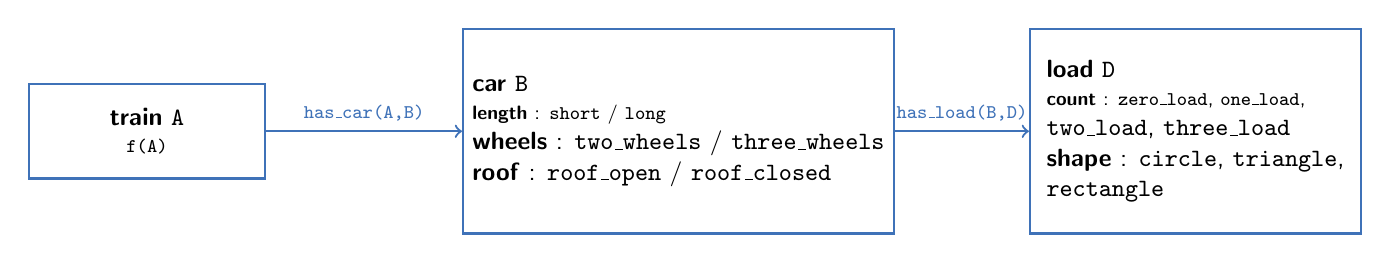
\begin{tikzpicture}[x=1cm,y=1cm, every node/.style={font=\small}]
  \node[draw=marine,fill=white,line width=0.9pt,minimum width=3.0cm,minimum height=1.2cm,align=center] (T) at (0,0) {\textbf{train} \texttt{A}\\[-1pt]{\scriptsize \texttt{f(A)}}};
  \node[draw=marine,fill=white,line width=0.9pt,minimum width=4.6cm,minimum height=2.6cm,align=left,anchor=west] (C) at (4.0,0) {\textbf{car} \texttt{B}\\[-1pt]
    \scriptsize \textbf{length} : \texttt{short} / \texttt{long}\\ \textbf{wheels} : \texttt{two\_wheels} / \texttt{three\_wheels}\\ \textbf{roof} : \texttt{roof\_open} / \texttt{roof\_closed}};
  \node[draw=marine,fill=white,line width=0.9pt,minimum width=4.2cm,minimum height=2.6cm,align=left,anchor=west] (L) at (11.2,0) {\textbf{load} \texttt{D}\\[-1pt]
    \scriptsize \textbf{count} : \texttt{zero\_load}, \texttt{one\_load},\\ \texttt{two\_load}, \texttt{three\_load}\\ \textbf{shape} : \texttt{circle}, \texttt{triangle},\\ \texttt{rectangle}};
  \draw[->,thick,marine] (T.east) -- node[above,font=\scriptsize\ttfamily]{has\_car(A,B)} (C.west);
  \draw[->,thick,marine] (C.east) -- node[above,font=\scriptsize\ttfamily]{has\_load(B,D)} (L.west);
\end{tikzpicture}
\end{center}
\ce{un train a plusieurs wagons (\texttt{has\_car}), un wagon a plusieurs chargements (\texttt{has\_load}). Les propriétés sont des prédicats unaires : \texttt{short(B)} veut dire ``le wagon \texttt{B} est court''.}

\st{Ce que Popper a le droit d'utiliser (\texttt{bias.pl})}
\renewcommand{\arraystretch}{1.25}
\begin{tabular}{@{}L{3.4cm}L{2.6cm}L{2.2cm}L{6.4cm}@{}}
\textbf{Predicate} & \textbf{Type} & \textbf{Direction} & \textbf{Rôle}\\\hline
\texttt{f/1} (head) & \texttt{(train)} & \texttt{(in)} & ce qu'on apprend : ``le train \texttt{A} est positif''\\
\texttt{has\_car/2} & \texttt{(train,car)} & \texttt{(in,out)} & donne un wagon d'un train\\
\texttt{has\_load/2} & \texttt{(car,load)} & \texttt{(in,out)} & donne un chargement d'un wagon\\
14 prédicats unaires & \texttt{(car)} ou \texttt{(load)} & \texttt{(in)} & propriétés testées sur un wagon ou un chargement\\
\end{tabular}
\ce{les directions sont celles de l'Assumption 3 : \texttt{has\_car(in,out)} \emph{produit} le wagon \texttt{B}, puis \texttt{short(in)} le \emph{lit}. C'est pour cela que \texttt{f(A) :- has\_car(A,B), short(B).} respecte les directions, et pas \texttt{f(A) :- short(B).}}
Le biais fixe aussi la taille de l'espace : \texttt{max\_clauses(3)}, \texttt{max\_vars(5)}, \texttt{max\_body(6)}, soit 1433 programmes de taille 3 à 6.
Le fichier \texttt{bk.pl} contient aussi des propriétés que le biais n'expose pas (\texttt{roof\_flat}, \texttt{roof\_arc}, \texttt{roof\_jagged}, \texttt{diamond}, \texttt{hexagon}\ldots) : Popper ne peut pas s'en servir.

\titrebox{3}{The 10 trains (les exemples en dessin)}
Chaque rectangle est un wagon. \textbf{Long} = large, \textbf{short} = étroit. Les ronds en bas sont les roues (2 ou 3). Une barre noire sur le dessus = toit fermé (\texttt{roof\_closed}), pas de barre = toit ouvert.
Les petites formes dans le wagon sont les chargements. Le petit bloc sombre à gauche est la locomotive.
\vspace{4pt}
\begin{center}
\begin{minipage}[t]{0.49\textwidth}
\centering{\large\bfseries\textcolor{marine}{Positive examples} ($E^+$)}\par\vspace{3pt}
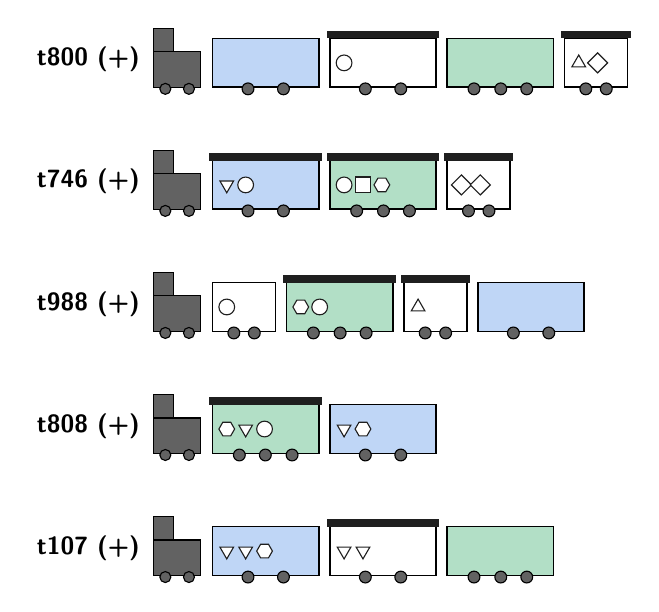
\begin{tikzpicture}[x=1cm,y=1cm]
\node[anchor=east,font=\small\bfseries] at (0.95,0.35) {t800 (+)};
\draw[fill=encre!70] (1.0,-0.00) rectangle (1.6,0.45); \draw[fill=encre!70] (1.0,0.45) rectangle (1.25,0.75);
\draw[fill=encre!70] (1.15,-0.02) circle (0.07); \draw[fill=encre!70] (1.45,-0.02) circle (0.07);
\draw[fill=pastel,line width=0.6pt] (1.75,-0.00) rectangle (3.10,0.62);
\draw[fill=encre!70] (2.20,-0.02) circle (0.075);
\draw[fill=encre!70] (2.65,-0.02) circle (0.075);
\draw[fill=white,line width=0.6pt] (3.24,-0.00) rectangle (4.59,0.62);
\fill[encre] (3.20,0.62) rectangle (4.63,0.72);
\draw[fill=encre!70] (3.69,-0.02) circle (0.075);
\draw[fill=encre!70] (4.14,-0.02) circle (0.075);
\node[draw=encre,fill=white,circle,inner sep=0pt,minimum size=0.2cm,line width=0.4pt] at (3.42,0.31) {};
\draw[fill=vert!35,line width=0.6pt] (4.73,-0.00) rectangle (6.08,0.62);
\draw[fill=encre!70] (5.07,-0.02) circle (0.075);
\draw[fill=encre!70] (5.41,-0.02) circle (0.075);
\draw[fill=encre!70] (5.74,-0.02) circle (0.075);
\draw[fill=white,line width=0.6pt] (6.22,-0.00) rectangle (7.02,0.62);
\fill[encre] (6.18,0.62) rectangle (7.06,0.72);
\draw[fill=encre!70] (6.49,-0.02) circle (0.075);
\draw[fill=encre!70] (6.75,-0.02) circle (0.075);
\node[draw=encre,fill=white,regular polygon,regular polygon sides=3,inner sep=0pt,minimum size=0.2cm,line width=0.4pt] at (6.40,0.31) {};
\node[draw=encre,fill=white,diamond,inner sep=0pt,minimum size=0.26cm,line width=0.4pt] at (6.64,0.31) {};
\node[anchor=east,font=\small\bfseries] at (0.95,-1.20) {t746 (+)};
\draw[fill=encre!70] (1.0,-1.55) rectangle (1.6,-1.10); \draw[fill=encre!70] (1.0,-1.10) rectangle (1.25,-0.80);
\draw[fill=encre!70] (1.15,-1.57) circle (0.07); \draw[fill=encre!70] (1.45,-1.57) circle (0.07);
\draw[fill=pastel,line width=0.6pt] (1.75,-1.55) rectangle (3.10,-0.93);
\fill[encre] (1.71,-0.93) rectangle (3.14,-0.83);
\draw[fill=encre!70] (2.20,-1.57) circle (0.075);
\draw[fill=encre!70] (2.65,-1.57) circle (0.075);
\node[draw=encre,fill=white,regular polygon,regular polygon sides=3,shape border rotate=180,inner sep=0pt,minimum size=0.2cm,line width=0.4pt] at (1.93,-1.24) {};
\node[draw=encre,fill=white,circle,inner sep=0pt,minimum size=0.2cm,line width=0.4pt] at (2.17,-1.24) {};
\draw[fill=vert!35,line width=0.6pt] (3.24,-1.55) rectangle (4.59,-0.93);
\fill[encre] (3.20,-0.93) rectangle (4.63,-0.83);
\draw[fill=encre!70] (3.58,-1.57) circle (0.075);
\draw[fill=encre!70] (3.92,-1.57) circle (0.075);
\draw[fill=encre!70] (4.25,-1.57) circle (0.075);
\node[draw=encre,fill=white,circle,inner sep=0pt,minimum size=0.2cm,line width=0.4pt] at (3.42,-1.24) {};
\node[draw=encre,fill=white,rectangle,inner sep=0pt,minimum size=0.2cm,line width=0.4pt] at (3.66,-1.24) {};
\node[draw=encre,fill=white,regular polygon,regular polygon sides=6,inner sep=0pt,minimum size=0.2cm,line width=0.4pt] at (3.90,-1.24) {};
\draw[fill=white,line width=0.6pt] (4.73,-1.55) rectangle (5.53,-0.93);
\fill[encre] (4.69,-0.93) rectangle (5.57,-0.83);
\draw[fill=encre!70] (5.00,-1.57) circle (0.075);
\draw[fill=encre!70] (5.26,-1.57) circle (0.075);
\node[draw=encre,fill=white,diamond,inner sep=0pt,minimum size=0.26cm,line width=0.4pt] at (4.91,-1.24) {};
\node[draw=encre,fill=white,diamond,inner sep=0pt,minimum size=0.26cm,line width=0.4pt] at (5.15,-1.24) {};
\node[anchor=east,font=\small\bfseries] at (0.95,-2.75) {t988 (+)};
\draw[fill=encre!70] (1.0,-3.10) rectangle (1.6,-2.65); \draw[fill=encre!70] (1.0,-2.65) rectangle (1.25,-2.35);
\draw[fill=encre!70] (1.15,-3.12) circle (0.07); \draw[fill=encre!70] (1.45,-3.12) circle (0.07);
\draw[fill=white,line width=0.6pt] (1.75,-3.10) rectangle (2.55,-2.48);
\draw[fill=encre!70] (2.02,-3.12) circle (0.075);
\draw[fill=encre!70] (2.28,-3.12) circle (0.075);
\node[draw=encre,fill=white,circle,inner sep=0pt,minimum size=0.2cm,line width=0.4pt] at (1.93,-2.79) {};
\draw[fill=vert!35,line width=0.6pt] (2.69,-3.10) rectangle (4.04,-2.48);
\fill[encre] (2.65,-2.48) rectangle (4.08,-2.38);
\draw[fill=encre!70] (3.03,-3.12) circle (0.075);
\draw[fill=encre!70] (3.37,-3.12) circle (0.075);
\draw[fill=encre!70] (3.70,-3.12) circle (0.075);
\node[draw=encre,fill=white,regular polygon,regular polygon sides=6,inner sep=0pt,minimum size=0.2cm,line width=0.4pt] at (2.87,-2.79) {};
\node[draw=encre,fill=white,circle,inner sep=0pt,minimum size=0.2cm,line width=0.4pt] at (3.11,-2.79) {};
\draw[fill=white,line width=0.6pt] (4.18,-3.10) rectangle (4.98,-2.48);
\fill[encre] (4.14,-2.48) rectangle (5.02,-2.38);
\draw[fill=encre!70] (4.45,-3.12) circle (0.075);
\draw[fill=encre!70] (4.71,-3.12) circle (0.075);
\node[draw=encre,fill=white,regular polygon,regular polygon sides=3,inner sep=0pt,minimum size=0.2cm,line width=0.4pt] at (4.36,-2.79) {};
\draw[fill=pastel,line width=0.6pt] (5.12,-3.10) rectangle (6.47,-2.48);
\draw[fill=encre!70] (5.57,-3.12) circle (0.075);
\draw[fill=encre!70] (6.02,-3.12) circle (0.075);
\node[anchor=east,font=\small\bfseries] at (0.95,-4.30) {t808 (+)};
\draw[fill=encre!70] (1.0,-4.65) rectangle (1.6,-4.20); \draw[fill=encre!70] (1.0,-4.20) rectangle (1.25,-3.90);
\draw[fill=encre!70] (1.15,-4.67) circle (0.07); \draw[fill=encre!70] (1.45,-4.67) circle (0.07);
\draw[fill=vert!35,line width=0.6pt] (1.75,-4.65) rectangle (3.10,-4.03);
\fill[encre] (1.71,-4.03) rectangle (3.14,-3.93);
\draw[fill=encre!70] (2.09,-4.67) circle (0.075);
\draw[fill=encre!70] (2.42,-4.67) circle (0.075);
\draw[fill=encre!70] (2.76,-4.67) circle (0.075);
\node[draw=encre,fill=white,regular polygon,regular polygon sides=6,inner sep=0pt,minimum size=0.2cm,line width=0.4pt] at (1.93,-4.34) {};
\node[draw=encre,fill=white,regular polygon,regular polygon sides=3,shape border rotate=180,inner sep=0pt,minimum size=0.2cm,line width=0.4pt] at (2.17,-4.34) {};
\node[draw=encre,fill=white,circle,inner sep=0pt,minimum size=0.2cm,line width=0.4pt] at (2.41,-4.34) {};
\draw[fill=pastel,line width=0.6pt] (3.24,-4.65) rectangle (4.59,-4.03);
\draw[fill=encre!70] (3.69,-4.67) circle (0.075);
\draw[fill=encre!70] (4.14,-4.67) circle (0.075);
\node[draw=encre,fill=white,regular polygon,regular polygon sides=3,shape border rotate=180,inner sep=0pt,minimum size=0.2cm,line width=0.4pt] at (3.42,-4.34) {};
\node[draw=encre,fill=white,regular polygon,regular polygon sides=6,inner sep=0pt,minimum size=0.2cm,line width=0.4pt] at (3.66,-4.34) {};
\node[anchor=east,font=\small\bfseries] at (0.95,-5.85) {t107 (+)};
\draw[fill=encre!70] (1.0,-6.20) rectangle (1.6,-5.75); \draw[fill=encre!70] (1.0,-5.75) rectangle (1.25,-5.45);
\draw[fill=encre!70] (1.15,-6.22) circle (0.07); \draw[fill=encre!70] (1.45,-6.22) circle (0.07);
\draw[fill=pastel,line width=0.6pt] (1.75,-6.20) rectangle (3.10,-5.58);
\draw[fill=encre!70] (2.20,-6.22) circle (0.075);
\draw[fill=encre!70] (2.65,-6.22) circle (0.075);
\node[draw=encre,fill=white,regular polygon,regular polygon sides=3,shape border rotate=180,inner sep=0pt,minimum size=0.2cm,line width=0.4pt] at (1.93,-5.89) {};
\node[draw=encre,fill=white,regular polygon,regular polygon sides=3,shape border rotate=180,inner sep=0pt,minimum size=0.2cm,line width=0.4pt] at (2.17,-5.89) {};
\node[draw=encre,fill=white,regular polygon,regular polygon sides=6,inner sep=0pt,minimum size=0.2cm,line width=0.4pt] at (2.41,-5.89) {};
\draw[fill=white,line width=0.6pt] (3.24,-6.20) rectangle (4.59,-5.58);
\fill[encre] (3.20,-5.58) rectangle (4.63,-5.48);
\draw[fill=encre!70] (3.69,-6.22) circle (0.075);
\draw[fill=encre!70] (4.14,-6.22) circle (0.075);
\node[draw=encre,fill=white,regular polygon,regular polygon sides=3,shape border rotate=180,inner sep=0pt,minimum size=0.2cm,line width=0.4pt] at (3.42,-5.89) {};
\node[draw=encre,fill=white,regular polygon,regular polygon sides=3,shape border rotate=180,inner sep=0pt,minimum size=0.2cm,line width=0.4pt] at (3.66,-5.89) {};
\draw[fill=vert!35,line width=0.6pt] (4.73,-6.20) rectangle (6.08,-5.58);
\draw[fill=encre!70] (5.07,-6.22) circle (0.075);
\draw[fill=encre!70] (5.41,-6.22) circle (0.075);
\draw[fill=encre!70] (5.74,-6.22) circle (0.075);
\end{tikzpicture}
\end{minipage}\hfill
\begin{minipage}[t]{0.49\textwidth}
\centering{\large\bfseries\textcolor{rouge}{Negative examples} ($E^-$)}\par\vspace{3pt}
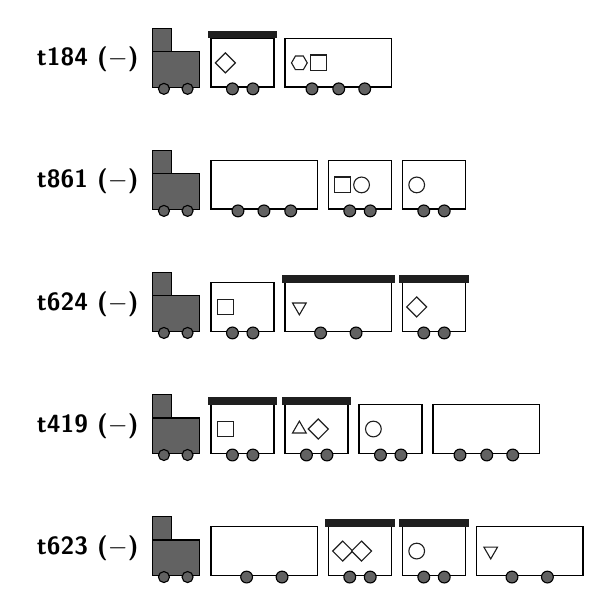
\begin{tikzpicture}[x=1cm,y=1cm]
\node[anchor=east,font=\small\bfseries] at (0.95,0.35) {t184 ($-$)};
\draw[fill=encre!70] (1.0,-0.00) rectangle (1.6,0.45); \draw[fill=encre!70] (1.0,0.45) rectangle (1.25,0.75);
\draw[fill=encre!70] (1.15,-0.02) circle (0.07); \draw[fill=encre!70] (1.45,-0.02) circle (0.07);
\draw[fill=white,line width=0.6pt] (1.75,-0.00) rectangle (2.55,0.62);
\fill[encre] (1.71,0.62) rectangle (2.59,0.72);
\draw[fill=encre!70] (2.02,-0.02) circle (0.075);
\draw[fill=encre!70] (2.28,-0.02) circle (0.075);
\node[draw=encre,fill=white,diamond,inner sep=0pt,minimum size=0.26cm,line width=0.4pt] at (1.93,0.31) {};
\draw[fill=white,line width=0.6pt] (2.69,-0.00) rectangle (4.04,0.62);
\draw[fill=encre!70] (3.03,-0.02) circle (0.075);
\draw[fill=encre!70] (3.37,-0.02) circle (0.075);
\draw[fill=encre!70] (3.70,-0.02) circle (0.075);
\node[draw=encre,fill=white,regular polygon,regular polygon sides=6,inner sep=0pt,minimum size=0.2cm,line width=0.4pt] at (2.87,0.31) {};
\node[draw=encre,fill=white,rectangle,inner sep=0pt,minimum size=0.2cm,line width=0.4pt] at (3.11,0.31) {};
\node[anchor=east,font=\small\bfseries] at (0.95,-1.20) {t861 ($-$)};
\draw[fill=encre!70] (1.0,-1.55) rectangle (1.6,-1.10); \draw[fill=encre!70] (1.0,-1.10) rectangle (1.25,-0.80);
\draw[fill=encre!70] (1.15,-1.57) circle (0.07); \draw[fill=encre!70] (1.45,-1.57) circle (0.07);
\draw[fill=white,line width=0.6pt] (1.75,-1.55) rectangle (3.10,-0.93);
\draw[fill=encre!70] (2.09,-1.57) circle (0.075);
\draw[fill=encre!70] (2.42,-1.57) circle (0.075);
\draw[fill=encre!70] (2.76,-1.57) circle (0.075);
\draw[fill=white,line width=0.6pt] (3.24,-1.55) rectangle (4.04,-0.93);
\draw[fill=encre!70] (3.51,-1.57) circle (0.075);
\draw[fill=encre!70] (3.77,-1.57) circle (0.075);
\node[draw=encre,fill=white,rectangle,inner sep=0pt,minimum size=0.2cm,line width=0.4pt] at (3.42,-1.24) {};
\node[draw=encre,fill=white,circle,inner sep=0pt,minimum size=0.2cm,line width=0.4pt] at (3.66,-1.24) {};
\draw[fill=white,line width=0.6pt] (4.18,-1.55) rectangle (4.98,-0.93);
\draw[fill=encre!70] (4.45,-1.57) circle (0.075);
\draw[fill=encre!70] (4.71,-1.57) circle (0.075);
\node[draw=encre,fill=white,circle,inner sep=0pt,minimum size=0.2cm,line width=0.4pt] at (4.36,-1.24) {};
\node[anchor=east,font=\small\bfseries] at (0.95,-2.75) {t624 ($-$)};
\draw[fill=encre!70] (1.0,-3.10) rectangle (1.6,-2.65); \draw[fill=encre!70] (1.0,-2.65) rectangle (1.25,-2.35);
\draw[fill=encre!70] (1.15,-3.12) circle (0.07); \draw[fill=encre!70] (1.45,-3.12) circle (0.07);
\draw[fill=white,line width=0.6pt] (1.75,-3.10) rectangle (2.55,-2.48);
\draw[fill=encre!70] (2.02,-3.12) circle (0.075);
\draw[fill=encre!70] (2.28,-3.12) circle (0.075);
\node[draw=encre,fill=white,rectangle,inner sep=0pt,minimum size=0.2cm,line width=0.4pt] at (1.93,-2.79) {};
\draw[fill=white,line width=0.6pt] (2.69,-3.10) rectangle (4.04,-2.48);
\fill[encre] (2.65,-2.48) rectangle (4.08,-2.38);
\draw[fill=encre!70] (3.14,-3.12) circle (0.075);
\draw[fill=encre!70] (3.59,-3.12) circle (0.075);
\node[draw=encre,fill=white,regular polygon,regular polygon sides=3,shape border rotate=180,inner sep=0pt,minimum size=0.2cm,line width=0.4pt] at (2.87,-2.79) {};
\draw[fill=white,line width=0.6pt] (4.18,-3.10) rectangle (4.98,-2.48);
\fill[encre] (4.14,-2.48) rectangle (5.02,-2.38);
\draw[fill=encre!70] (4.45,-3.12) circle (0.075);
\draw[fill=encre!70] (4.71,-3.12) circle (0.075);
\node[draw=encre,fill=white,diamond,inner sep=0pt,minimum size=0.26cm,line width=0.4pt] at (4.36,-2.79) {};
\node[anchor=east,font=\small\bfseries] at (0.95,-4.30) {t419 ($-$)};
\draw[fill=encre!70] (1.0,-4.65) rectangle (1.6,-4.20); \draw[fill=encre!70] (1.0,-4.20) rectangle (1.25,-3.90);
\draw[fill=encre!70] (1.15,-4.67) circle (0.07); \draw[fill=encre!70] (1.45,-4.67) circle (0.07);
\draw[fill=white,line width=0.6pt] (1.75,-4.65) rectangle (2.55,-4.03);
\fill[encre] (1.71,-4.03) rectangle (2.59,-3.93);
\draw[fill=encre!70] (2.02,-4.67) circle (0.075);
\draw[fill=encre!70] (2.28,-4.67) circle (0.075);
\node[draw=encre,fill=white,rectangle,inner sep=0pt,minimum size=0.2cm,line width=0.4pt] at (1.93,-4.34) {};
\draw[fill=white,line width=0.6pt] (2.69,-4.65) rectangle (3.49,-4.03);
\fill[encre] (2.65,-4.03) rectangle (3.53,-3.93);
\draw[fill=encre!70] (2.96,-4.67) circle (0.075);
\draw[fill=encre!70] (3.22,-4.67) circle (0.075);
\node[draw=encre,fill=white,regular polygon,regular polygon sides=3,inner sep=0pt,minimum size=0.2cm,line width=0.4pt] at (2.87,-4.34) {};
\node[draw=encre,fill=white,diamond,inner sep=0pt,minimum size=0.26cm,line width=0.4pt] at (3.11,-4.34) {};
\draw[fill=white,line width=0.6pt] (3.63,-4.65) rectangle (4.43,-4.03);
\draw[fill=encre!70] (3.90,-4.67) circle (0.075);
\draw[fill=encre!70] (4.16,-4.67) circle (0.075);
\node[draw=encre,fill=white,circle,inner sep=0pt,minimum size=0.2cm,line width=0.4pt] at (3.81,-4.34) {};
\draw[fill=white,line width=0.6pt] (4.57,-4.65) rectangle (5.92,-4.03);
\draw[fill=encre!70] (4.91,-4.67) circle (0.075);
\draw[fill=encre!70] (5.25,-4.67) circle (0.075);
\draw[fill=encre!70] (5.58,-4.67) circle (0.075);
\node[anchor=east,font=\small\bfseries] at (0.95,-5.85) {t623 ($-$)};
\draw[fill=encre!70] (1.0,-6.20) rectangle (1.6,-5.75); \draw[fill=encre!70] (1.0,-5.75) rectangle (1.25,-5.45);
\draw[fill=encre!70] (1.15,-6.22) circle (0.07); \draw[fill=encre!70] (1.45,-6.22) circle (0.07);
\draw[fill=white,line width=0.6pt] (1.75,-6.20) rectangle (3.10,-5.58);
\draw[fill=encre!70] (2.20,-6.22) circle (0.075);
\draw[fill=encre!70] (2.65,-6.22) circle (0.075);
\draw[fill=white,line width=0.6pt] (3.24,-6.20) rectangle (4.04,-5.58);
\fill[encre] (3.20,-5.58) rectangle (4.08,-5.48);
\draw[fill=encre!70] (3.51,-6.22) circle (0.075);
\draw[fill=encre!70] (3.77,-6.22) circle (0.075);
\node[draw=encre,fill=white,diamond,inner sep=0pt,minimum size=0.26cm,line width=0.4pt] at (3.42,-5.89) {};
\node[draw=encre,fill=white,diamond,inner sep=0pt,minimum size=0.26cm,line width=0.4pt] at (3.66,-5.89) {};
\draw[fill=white,line width=0.6pt] (4.18,-6.20) rectangle (4.98,-5.58);
\fill[encre] (4.14,-5.58) rectangle (5.02,-5.48);
\draw[fill=encre!70] (4.45,-6.22) circle (0.075);
\draw[fill=encre!70] (4.71,-6.22) circle (0.075);
\node[draw=encre,fill=white,circle,inner sep=0pt,minimum size=0.2cm,line width=0.4pt] at (4.36,-5.89) {};
\draw[fill=white,line width=0.6pt] (5.12,-6.20) rectangle (6.47,-5.58);
\draw[fill=encre!70] (5.57,-6.22) circle (0.075);
\draw[fill=encre!70] (6.02,-6.22) circle (0.075);
\node[draw=encre,fill=white,regular polygon,regular polygon sides=3,shape border rotate=180,inner sep=0pt,minimum size=0.2cm,line width=0.4pt] at (5.30,-5.89) {};
\end{tikzpicture}
\end{minipage}
\end{center}
\vspace{2pt}
\textbf{Légende des couleurs (positifs) :} \colorbox{vert!35}{\strut wagon à 3 roues} \quad \colorbox{pastel}{\strut wagon long à 2 roues}.
Ces deux wagons sont ceux que la règle ci-dessous utilise comme témoins.

\titrebox{4}{The hidden rule (la règle cachée)}
\st{Ce que Popper trouve (tour 48)}
\begin{moi}
\texttt{f(A) :- has\_car(A,B), has\_car(A,C), long(C), three\_wheels(B), two\_wheels(C).}
\end{moi}
En français : \emph{un train est positif s'il a un wagon à trois roues et un autre wagon long à deux roues.}
Sur les 10 exemples : TP\,=\,5, FN\,=\,0, FP\,=\,0, TN\,=\,5, donc l'issue est (ALL, NONE) et Popper s'arrête.

\st{Une autre règle parfaite sur ces 10 trains}
\begin{moi}
\texttt{f(A) :- has\_car(A,C), long(C), roof\_closed(C), has\_car(A,B), three\_wheels(B).}
\end{moi}
En français : \emph{un train est positif s'il a un wagon long à toit fermé et un wagon à trois roues.} C'est la règle donnée en commentaire dans le \texttt{bias.pl} du dataset.
\begin{piege}
Avec seulement 10 exemples, \textbf{plusieurs règles de même taille (6 littéraux) sont parfaites}. Popper renvoie la première qu'il trouve, pas forcément celle que le concepteur du jeu de données avait en tête. Ce n'est pas une erreur : une solution est une règle complète et cohérente.
\end{piege}

\st{Vérification train par train}
\def\ok{\textcolor{vert}{\ding{51}}}\def\ko{\textcolor{rouge}{\ding{55}}}
\renewcommand{\arraystretch}{1.2}
\begin{tabular}{@{}l c c c c c@{}}
\textbf{Train} & \textbf{Label} & \textbf{Règle trouvée} & \textbf{Règle du \texttt{bias.pl}} & \texttt{has\_car,short} (\#1) & ``wagon court fermé''\\\hline
t800 & $+$ & \ok & \ok & \ok & \ok\\
t746 & $+$ & \ok & \ok & \ok & \ok\\
t988 & $+$ & \ok & \ok & \ok & \ok\\
t808 & $+$ & \ok & \ok & \ko & \ko\\
t107 & $+$ & \ok & \ok & \ko & \ko\\\hline
t184 & $-$ & \ko & \ko & \ok & \ok\\
t861 & $-$ & \ko & \ko & \ok & \ko\\
t624 & $-$ & \ko & \ko & \ok & \ok\\
t419 & $-$ & \ko & \ko & \ok & \ok\\
t623 & $-$ & \ko & \ko & \ok & \ok\\
\end{tabular}
\ce{une coche signifie ``le programme couvre ce train''. Une bonne règle a des coches sur les 5 positifs et aucune sur les négatifs. Les deux premières colonnes sont parfaites. \texttt{has\_car, short} (le programme \#1) couvre tous les négatifs, c'est pour cela qu'il est rejeté (3 positifs, 5 faux positifs). Même la règle classique ``un wagon court fermé'' est fausse ici.}

\titrebox{5}{Lien avec la preuve (federated)}
\st{La partition en 3 clients (\texttt{iid\_3\_seed\_42})}
\renewcommand{\arraystretch}{1.25}
\begin{tabular}{@{}l L{5.4cm}L{5.4cm}@{}}
\textbf{Client} & \textbf{Positifs} & \textbf{Négatifs}\\\hline
C1 & t808, t107 & t419, t623\\
C2 & t746, t800 & t624, t861\\
C3 & t988 & t184\\
\end{tabular}
\begin{itemize}
  \item \textbf{A1 Example Locality} : les 5 positifs et les 5 négatifs sont répartis sans doublon, avec au moins un de chaque par client.
  \item \textbf{A2 Separated Local Constants} : chaque constante porte le nom de son train (\texttt{t800}, \texttt{t800\_c1}, \texttt{t800\_c1\_l1}). Aucune constante \emph{d'exemple} n'est partagée entre deux clients. En revanche, \textbf{chaque client contient aussi les 990 trains sans exemple}, copiés à l'identique (28\,226 faits) : ils jouent le rôle de $\mathcal{R}$ (partagé), et leurs constantes ne sont locales à aucun client.
  \item \textbf{A3 Directions} : \texttt{has\_car(in,out)}, \texttt{has\_load(in,out)}, et les 14 prédicats unaires en \texttt{in}. Tout littéral part donc de l'exemple.
\end{itemize}
\st{Pourquoi un client seul se trompe}
Avec le programme \#9 (\texttt{has\_load}, \texttt{three\_load}), le client C1 voit (ALL, NONE) : il croit à une solution. Mais le client C2 voit (NONE, NONE) pour ses positifs, et le global est (SOME, NONE) : la solution est incomplète. D'où la nécessité d'\textbf{agréger} les comptes.
\ce{le dataset Trains est un cas où les 3 assumptions sont vraies \emph{par construction} (identifiants préfixés par le train, directions déclarées dans \texttt{bias.pl}). C'est ce qui rend le théorème applicable ici.}

% =====================================================================
%  ANNEXE : le dataset Zendo
% =====================================================================
\partie{V}{Annexe : le dataset Zendo}{Comprendre le schéma des données, quelques exemples dessinés, les règles candidates et la règle finale. On ne parcourt pas les 40 exemples.}

\titrebox{1}{The task (la tâche)}
Zendo est un jeu : une \emph{structure} est un petit tas de pièces colorées posées sur une table, et un maître du jeu cache une règle qui dit quelles structures sont ``positives''.
Ici : 40 structures, 20 \EN{positive examples}{positifs} et 20 \EN{negative examples}{négatifs}. Le prédicat à apprendre est \texttt{zendo(S)} (``la structure \texttt{S} est positive'').
Popper ne connaît pas la règle : il ne voit que les faits.
\begin{moi}
\texttt{pos(zendo(0)). \ldots\ pos(zendo(19)).}\qquad \texttt{neg(zendo(20)). \ldots\ neg(zendo(39)).}
\end{moi}
\textbf{Taille :} 139 pièces au total, de 1 à 5 par structure (3,5 en moyenne), 60 faits \texttt{contact} distincts.
La source est l'article de Hocquette et Cropper (AAAI 2023, \emph{Relational Program Synthesis with Numerical Reasoning}), cité dans le \texttt{bias.pl}.

\titrebox{2}{The schema (le schéma) : structure, pièce, nombres}
\begin{center}
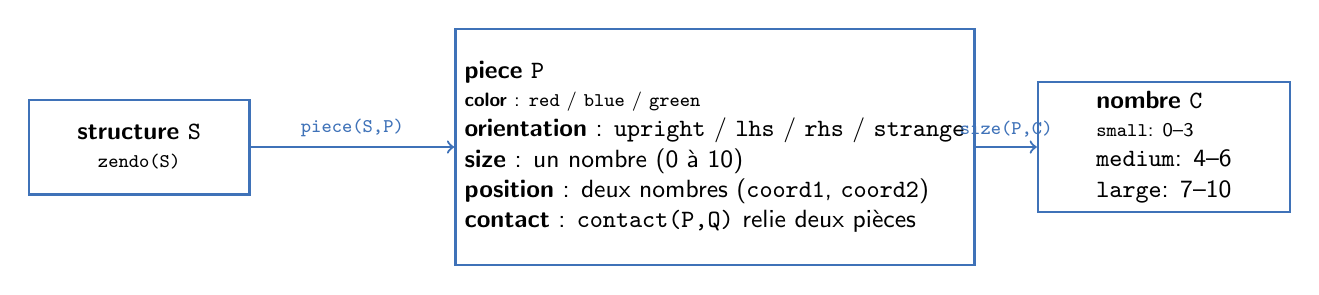
\begin{tikzpicture}[x=1cm,y=1cm, every node/.style={font=\small}]
  \node[draw=marine,fill=white,line width=0.9pt,minimum width=2.8cm,minimum height=1.2cm,align=center] (S) at (0,0) {\textbf{structure} \texttt{S}\\[-1pt]{\scriptsize \texttt{zendo(S)}}};
  \node[draw=marine,fill=white,line width=0.9pt,minimum width=5.8cm,minimum height=3.0cm,align=left,anchor=west] (P) at (4.0,0) {\textbf{piece} \texttt{P}\\[-1pt]
    \scriptsize \textbf{color} : \texttt{red} / \texttt{blue} / \texttt{green}\\ \textbf{orientation} : \texttt{upright} / \texttt{lhs} / \texttt{rhs} / \texttt{strange}\\ \textbf{size} : un nombre (0 à 10)\\ \textbf{position} : deux nombres (\texttt{coord1}, \texttt{coord2})\\ \textbf{contact} : \texttt{contact(P,Q)} relie deux pièces};
  \node[draw=marine,fill=white,line width=0.9pt,minimum width=3.2cm,minimum height=1.6cm,align=left,anchor=west] (N) at (11.4,0) {\textbf{nombre} \texttt{C}\\[-1pt]
    \scriptsize \texttt{small}: 0--3\\ \texttt{medium}: 4--6\\ \texttt{large}: 7--10};
  \draw[->,thick,marine] (S.east) -- node[above,font=\scriptsize\ttfamily]{piece(S,P)} (P.west);
  \draw[->,thick,marine] (P.east) -- node[above,font=\scriptsize\ttfamily]{size(P,C)} (N.west);
\end{tikzpicture}
\end{center}
\ce{une structure a des pièces (\texttt{piece}). Deux pièces peuvent se toucher (\texttt{contact(P,Q)}, un lien entre pièces). La taille est un \emph{nombre} : \texttt{size(P,C)} le renvoie, puis \texttt{small(C)}, \texttt{medium(C)} ou \texttt{large(C)} teste dans quelle tranche il se trouve. C'est la partie ``numérique'' du dataset.}

\st{Ce que Popper a le droit d'utiliser (\texttt{bias.pl})}
\renewcommand{\arraystretch}{1.25}
\begin{tabular}{@{}L{3.6cm}L{3.2cm}L{2.3cm}L{5.6cm}@{}}
\textbf{Predicate} & \textbf{Type} & \textbf{Direction} & \textbf{Rôle}\\\hline
\texttt{zendo/1} (head) & \texttt{(state)} & \texttt{(in)} & ce qu'on apprend\\
\texttt{piece/2} & \texttt{(state,piece)} & \texttt{(in,out)} & donne une pièce d'une structure\\
\texttt{contact/2} & \texttt{(piece,piece)} & \texttt{(in,out)} & donne une pièce qui touche la pièce d'entrée\\
\texttt{size/2}, \texttt{coord1/2}, \texttt{coord2/2} & \texttt{(piece,real)} & \texttt{(in,out)} & donne un nombre lié à la pièce\\
\texttt{small}, \texttt{medium}, \texttt{large} & \texttt{(real)} & \texttt{(in)} & teste un nombre\\
\texttt{red}, \texttt{blue}, \texttt{green}, \texttt{upright}, \texttt{lhs}, \texttt{rhs}, \texttt{strange} & \texttt{(piece)} & \texttt{(in)} & teste une propriété de la pièce\\
\end{tabular}
\ce{les directions sont celles de l'Assumption 3. Le biais impose aussi : une seule variable de type \texttt{state} par clause, \texttt{max\_clauses(4)}, \texttt{max\_vars(5)}, \texttt{max\_body(7)}.}

\titrebox{3}{Quatre structures dessinées (les exemples en dessin)}
Chaque triangle est une pièce. \textbf{Couleur} = couleur de la pièce, \textbf{taille du triangle} = \texttt{size} (le petit nombre à côté est la valeur), \textbf{direction de la pointe} = orientation (j'ai choisi :
\texttt{upright} vers le haut, \texttt{lhs} vers la gauche, \texttt{rhs} vers la droite, \texttt{strange} penché). La position suit \texttt{coord1} (horizontal) et \texttt{coord2} (vertical).
Un trait noir épais relie deux pièces en \texttt{contact}. Dans les positifs, le cercle pointillé entoure les deux pièces qui expliquent pourquoi la structure est positive.
\vspace{4pt}
\begin{center}
\begin{minipage}[t]{0.49\textwidth}\centering
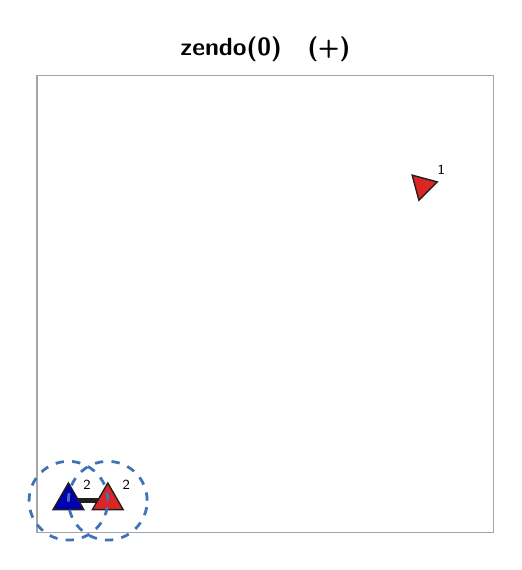
\begin{tikzpicture}[x=1cm,y=1cm]
\draw[encre!40,fill=white,line width=0.5pt] (-0.4,-0.4) rectangle (5.40,5.40);
\draw[encre,line width=1.6pt] (0.50,0.00) -- (0.00,0.00);
\node[regular polygon,regular polygon sides=3,shape border rotate=0,draw=encre,fill=rouge,line width=0.5pt,inner sep=0pt,minimum size=0.45cm] at (0.50,0.00) {};
\node[font=\tiny,above right=-1pt] at (0.60,0.05) {2};
\node[regular polygon,regular polygon sides=3,shape border rotate=45,draw=encre,fill=rouge,line width=0.5pt,inner sep=0pt,minimum size=0.38cm] at (4.50,4.00) {};
\node[font=\tiny,above right=-1pt] at (4.60,4.05) {1};
\node[regular polygon,regular polygon sides=3,shape border rotate=0,draw=encre,fill=blue!70!black,line width=0.5pt,inner sep=0pt,minimum size=0.45cm] at (0.00,0.00) {};
\node[font=\tiny,above right=-1pt] at (0.10,0.05) {2};
\draw[marine,dashed,line width=1pt] (0.00,0.00) circle (0.5);
\draw[marine,dashed,line width=1pt] (0.50,0.00) circle (0.5);
\node[anchor=south,font=\small\bfseries] at (2.50,5.45) {zendo(0) \; (+)};
\end{tikzpicture}
\end{minipage}\hfill
\begin{minipage}[t]{0.49\textwidth}\centering
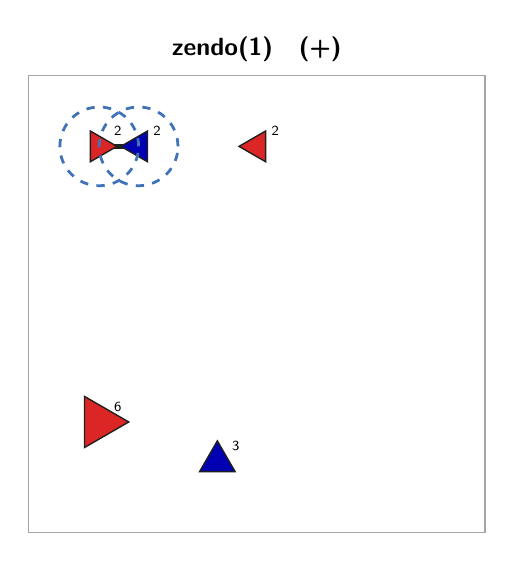
\begin{tikzpicture}[x=1cm,y=1cm]
\draw[encre!40,fill=white,line width=0.5pt] (-0.4,-0.4) rectangle (5.40,5.40);
\draw[encre,line width=1.6pt] (1.00,4.50) -- (0.50,4.50);
\node[regular polygon,regular polygon sides=3,shape border rotate=90,draw=encre,fill=rouge,line width=0.5pt,inner sep=0pt,minimum size=0.45cm] at (2.50,4.50) {};
\node[font=\tiny,above right=-1pt] at (2.60,4.55) {2};
\node[regular polygon,regular polygon sides=3,shape border rotate=-90,draw=encre,fill=rouge,line width=0.5pt,inner sep=0pt,minimum size=0.75cm] at (0.50,1.00) {};
\node[font=\tiny,above right=-1pt] at (0.60,1.05) {6};
\node[regular polygon,regular polygon sides=3,shape border rotate=90,draw=encre,fill=blue!70!black,line width=0.5pt,inner sep=0pt,minimum size=0.45cm] at (1.00,4.50) {};
\node[font=\tiny,above right=-1pt] at (1.10,4.55) {2};
\node[regular polygon,regular polygon sides=3,shape border rotate=0,draw=encre,fill=blue!70!black,line width=0.5pt,inner sep=0pt,minimum size=0.52cm] at (2.00,0.50) {};
\node[font=\tiny,above right=-1pt] at (2.10,0.55) {3};
\node[regular polygon,regular polygon sides=3,shape border rotate=-90,draw=encre,fill=rouge,line width=0.5pt,inner sep=0pt,minimum size=0.45cm] at (0.50,4.50) {};
\node[font=\tiny,above right=-1pt] at (0.60,4.55) {2};
\draw[marine,dashed,line width=1pt] (1.00,4.50) circle (0.5);
\draw[marine,dashed,line width=1pt] (0.50,4.50) circle (0.5);
\node[anchor=south,font=\small\bfseries] at (2.50,5.45) {zendo(1) \; (+)};
\end{tikzpicture}
\end{minipage}\\[10pt]
\begin{minipage}[t]{0.49\textwidth}\centering
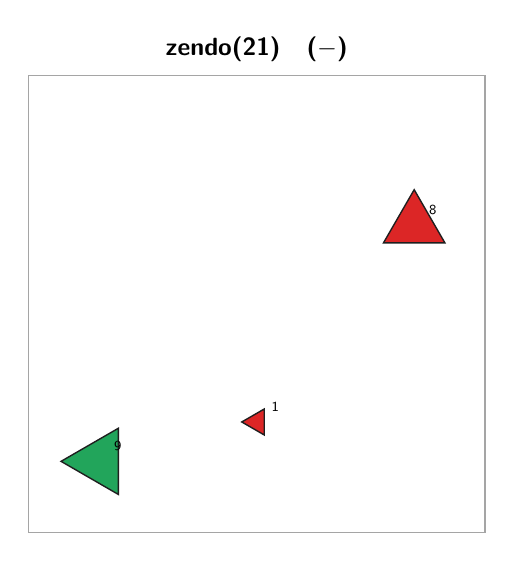
\begin{tikzpicture}[x=1cm,y=1cm]
\draw[encre!40,fill=white,line width=0.5pt] (-0.4,-0.4) rectangle (5.40,5.40);
\node[regular polygon,regular polygon sides=3,shape border rotate=90,draw=encre,fill=vert,line width=0.5pt,inner sep=0pt,minimum size=0.97cm] at (0.50,0.50) {};
\node[font=\tiny,above right=-1pt] at (0.60,0.55) {9};
\node[regular polygon,regular polygon sides=3,shape border rotate=0,draw=encre,fill=rouge,line width=0.5pt,inner sep=0pt,minimum size=0.90cm] at (4.50,3.50) {};
\node[font=\tiny,above right=-1pt] at (4.60,3.55) {8};
\node[regular polygon,regular polygon sides=3,shape border rotate=90,draw=encre,fill=rouge,line width=0.5pt,inner sep=0pt,minimum size=0.38cm] at (2.50,1.00) {};
\node[font=\tiny,above right=-1pt] at (2.60,1.05) {1};
\node[anchor=south,font=\small\bfseries] at (2.50,5.45) {zendo(21) \; ($-$)};
\end{tikzpicture}
\end{minipage}\hfill
\begin{minipage}[t]{0.49\textwidth}\centering
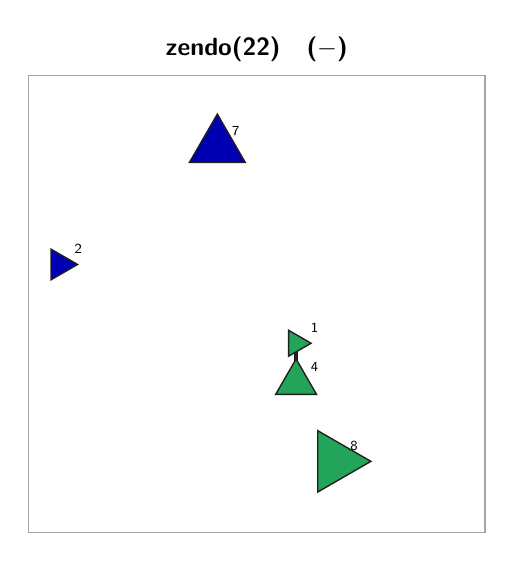
\begin{tikzpicture}[x=1cm,y=1cm]
\draw[encre!40,fill=white,line width=0.5pt] (-0.4,-0.4) rectangle (5.40,5.40);
\draw[encre,line width=1.6pt] (3.00,2.00) -- (3.00,1.50);
\node[regular polygon,regular polygon sides=3,shape border rotate=-90,draw=encre,fill=vert,line width=0.5pt,inner sep=0pt,minimum size=0.90cm] at (3.50,0.50) {};
\node[font=\tiny,above right=-1pt] at (3.60,0.55) {8};
\node[regular polygon,regular polygon sides=3,shape border rotate=-90,draw=encre,fill=vert,line width=0.5pt,inner sep=0pt,minimum size=0.38cm] at (3.00,2.00) {};
\node[font=\tiny,above right=-1pt] at (3.10,2.05) {1};
\node[regular polygon,regular polygon sides=3,shape border rotate=0,draw=encre,fill=blue!70!black,line width=0.5pt,inner sep=0pt,minimum size=0.82cm] at (2.00,4.50) {};
\node[font=\tiny,above right=-1pt] at (2.10,4.55) {7};
\node[regular polygon,regular polygon sides=3,shape border rotate=-90,draw=encre,fill=blue!70!black,line width=0.5pt,inner sep=0pt,minimum size=0.45cm] at (0.00,3.00) {};
\node[font=\tiny,above right=-1pt] at (0.10,3.05) {2};
\node[regular polygon,regular polygon sides=3,shape border rotate=0,draw=encre,fill=vert,line width=0.5pt,inner sep=0pt,minimum size=0.60cm] at (3.00,1.50) {};
\node[font=\tiny,above right=-1pt] at (3.10,1.55) {4};
\node[anchor=south,font=\small\bfseries] at (2.50,5.45) {zendo(22) \; ($-$)};
\end{tikzpicture}
\end{minipage}
\end{center}
\textbf{Comment lire :}
\begin{itemize}
  \item \textbf{zendo(0) (+)} : la pièce bleue de taille 2 (petite) touche la pièce rouge $\Rightarrow$ positif.
  \item \textbf{zendo(1) (+)} : la pièce bleue de taille 2 touche la pièce rouge de taille 2 $\Rightarrow$ positif.
  \item \textbf{zendo(21) ($-$)} : il y a des pièces rouges, mais \emph{aucun contact} $\Rightarrow$ négatif.
  \item \textbf{zendo(22) ($-$)} : une petite pièce touche une autre pièce, mais la pièce touchée est \emph{verte}, pas rouge $\Rightarrow$ négatif.
\end{itemize}

\titrebox{4}{The hidden rule (la règle cachée)}
\st{La règle finale}
\begin{moi}
\texttt{zendo(A) :- piece(A,B), size(B,C), small(C), contact(B,D), red(D).}
\end{moi}
En français : \emph{une structure est positive si elle contient une petite pièce qui touche une pièce rouge.}
C'est la règle donnée en commentaire dans le \texttt{bias.pl}. Je l'ai vérifiée sur les 40 structures : elle couvre les 20 positifs et aucun des 20 négatifs, donc (ALL, NONE).
Elle respecte les directions : \texttt{B} sort de \texttt{piece}, \texttt{C} sort de \texttt{size}, \texttt{D} sort de \texttt{contact}, et chaque variable est produite avant d'être lue.

\st{Pourquoi il faut les deux conditions : règles incomplètes}
Une règle trop simple couvre aussi des négatifs. Résultats mesurés sur les 20 positifs et les 20 négatifs :
\renewcommand{\arraystretch}{1.25}
\begin{center}
\begin{tabular}{@{}L{8.6cm}c c l@{}}
\textbf{Règle candidate} & \textbf{positifs couverts} & \textbf{négatifs couverts} & \textbf{issue}\\\hline
la structure a une pièce rouge & 20 / 20 & 12 / 20 & (ALL, SOME)\\
la structure a une petite pièce & 20 / 20 & 17 / 20 & (ALL, SOME)\\
deux pièces se touchent & 20 / 20 & 4 / 20 & (ALL, SOME)\\
une petite pièce en touche une autre & 20 / 20 & 4 / 20 & (ALL, SOME)\\
une pièce en touche une rouge & 20 / 20 & 1 / 20 & (ALL, SOME)\\
\textbf{une petite pièce touche une pièce rouge} & \textbf{20 / 20} & \textbf{0 / 20} & \textbf{(ALL, NONE)}\\
\end{tabular}
\end{center}
\ce{chaque condition retire des faux positifs. Dans la boucle de Popper, ce sont des programmes (ALL, SOME) : trop généraux, donc on interdit leurs généralisations (contraintes de \emph{generalisation}) et on cherche des programmes plus spécifiques jusqu'à (ALL, NONE).}

\titrebox{5}{Point de vigilance pour la preuve federated}
Dans Zendo, les identifiants de structure sont des nombres (\texttt{0} à \texttt{39}) et la taille ou la position sont aussi des nombres (\texttt{0} à \texttt{10}). Les pièces portent des noms locaux (\texttt{p0\_2}), mais \textbf{les nombres sont partagés entre structures}, donc entre clients.
\begin{piege}
\textbf{A2 (Separated Local Constants) ne tient donc pas à la lettre sur Zendo} : une constante comme \texttt{2} apparaît dans les faits \texttt{size(\ldots,2)} de plusieurs clients. Les \emph{types} du biais (\texttt{state}, \texttt{piece}, \texttt{real}) empêchent qu'un nombre de taille serve de point de départ pour un \texttt{piece(in,out)}, mais la preuve de la Part~I raisonne sans types. Avant d'utiliser Zendo comme exemple d'application du théorème, il faut soit raffiner A2 (constantes \emph{typées}), soit renommer les identifiants de structure. À vérifier.
\end{piege}

% =====================================================================
%  ANNEXE : le dataset IGGP Rock-Paper-Scissors
% =====================================================================
\partie{VI}{Annexe : le dataset iggp-rps}{Pierre-papier-ciseaux (IGGP). Schéma des données, tours de jeu dessinés, les règles $\mathcal{R}$ du background knowledge, et le programme appris.}

\titrebox{1}{The task (la tâche)}
Le dataset \texttt{iggp-rps} décrit une partie de \EN{rock-paper-scissors}{pierre-papier-ciseaux} entre deux joueurs, \texttt{p1} et \texttt{p2}, sur 58 tours. À chaque tour, chaque joueur choisit
\texttt{stone}, \texttt{paper} ou \texttt{scissors}. Le vainqueur gagne un point (\texttt{paper} bat \texttt{stone}, \texttt{scissors} bat \texttt{paper}, \texttt{stone} bat \texttt{scissors}), et l'égalité ne change rien.
Popper ne connaît pas ces règles du jeu : il doit les \emph{apprendre} à partir des exemples. Le nom \texttt{iggp} vient du benchmark \emph{Inductive General Game Playing} (à citer : vérifier la référence exacte).
\begin{moi}
\textbf{But à apprendre :} \texttt{next\_score(E,P,S)} : \emph{au tour \texttt{E}, le score du joueur \texttt{P} devient \texttt{S} au tour suivant.}
\end{moi}
\textbf{Taille :} 108 positifs et 356 négatifs. Chaque tour a deux positifs (la vraie valeur pour p1 et pour p2) ; les négatifs sont les mauvaises valeurs.
Les tours 2, 5, 8 et 14 n'ont \emph{aucun fait} \texttt{does} : ils n'ont pas de positif, seulement 8 négatifs chacun (32 négatifs).
\begin{center}
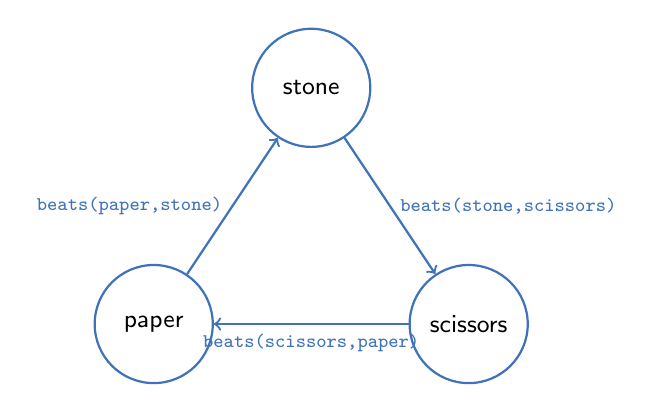
\begin{tikzpicture}[x=1cm,y=1cm,every node/.style={font=\small}]
  \node[draw=marine,fill=white,line width=0.8pt,circle,minimum size=1.5cm] (S) at (0,2.1) {stone};
  \node[draw=marine,fill=white,line width=0.8pt,circle,minimum size=1.5cm] (P) at (-2.0,-0.9) {paper};
  \node[draw=marine,fill=white,line width=0.8pt,circle,minimum size=1.5cm] (C) at (2.0,-0.9) {scissors};
  \draw[->,thick,marine] (P) -- node[left,font=\scriptsize\ttfamily]{beats(paper,stone)} (S);
  \draw[->,thick,marine] (S) -- node[right,font=\scriptsize\ttfamily]{beats(stone,scissors)} (C);
  \draw[->,thick,marine] (C) -- node[below,font=\scriptsize\ttfamily]{beats(scissors,paper)} (P);
\end{tikzpicture}
\end{center}
Une flèche $a\to b$ se lit : ``$a$ bat $b$''. Ces 3 faits \texttt{beats} sont dans le BK.

\titrebox{2}{The schema (le schéma) : le tour, les joueurs, les scores}
\begin{center}
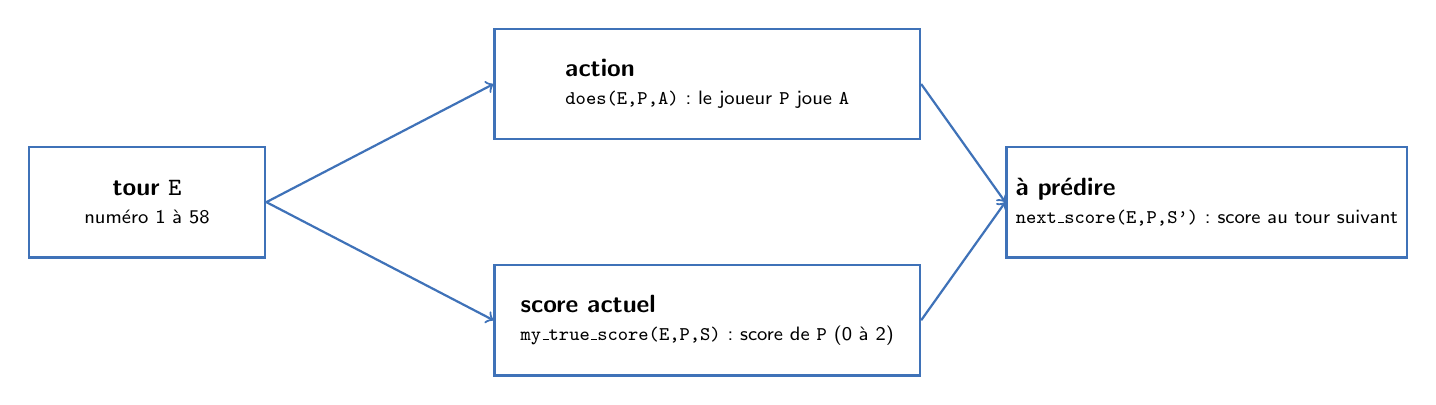
\begin{tikzpicture}[x=1cm,y=1cm, every node/.style={font=\small}]
  \node[draw=marine,fill=white,line width=0.9pt,minimum width=3.0cm,minimum height=1.4cm,align=center] (R) at (0,0) {\textbf{tour} \texttt{E}\\[-1pt]\scriptsize numéro 1 à 58};
  \node[draw=marine,fill=white,line width=0.9pt,minimum width=5.4cm,minimum height=1.4cm,align=left,anchor=west] (D) at (4.4,1.5) {\textbf{action}\\[-1pt]\scriptsize \texttt{does(E,P,A)} : le joueur \texttt{P} joue \texttt{A}};
  \node[draw=marine,fill=white,line width=0.9pt,minimum width=5.4cm,minimum height=1.4cm,align=left,anchor=west] (Sc) at (4.4,-1.5) {\textbf{score actuel}\\[-1pt]\scriptsize \texttt{my\_true\_score(E,P,S)} : score de \texttt{P} (0 à 2)};
  \node[draw=marine,fill=white,line width=0.9pt,minimum width=4.0cm,minimum height=1.4cm,align=left,anchor=west] (N) at (10.9,0) {\textbf{à prédire}\\[-1pt]\scriptsize \texttt{next\_score(E,P,S')} : score au tour suivant};
  \draw[->,thick,marine] (R.east) -- (D.west);
  \draw[->,thick,marine] (R.east) -- (Sc.west);
  \draw[->,thick,marine] (D.east) -- (N.west);
  \draw[->,thick,marine] (Sc.east) -- (N.west);
\end{tikzpicture}
\end{center}
\ce{tout ce qui change d'un tour à l'autre (\texttt{does}, \texttt{my\_true\_score}) a le numéro du tour \texttt{E} en \emph{premier argument}. Ce qui ne change jamais (\texttt{beats}, \texttt{my\_succ}, \texttt{player}, \texttt{different}) ne mentionne aucun tour.}

\st{Le background knowledge (\texttt{bk.pl}), trois catégories}
\renewcommand{\arraystretch}{1.25}
\begin{tabular}{@{}L{4.2cm}L{5.4cm}L{6.4cm}@{}}
\textbf{Catégorie} & \textbf{Contenu} & \textbf{Rôle}\\\hline
Faits \emph{par tour} & \texttt{does} (108 faits, 54 tours), \texttt{my\_true\_score} (116 faits, 58 tours), \texttt{my\_true\_step} (58 faits) & les données propres à chaque tour. \texttt{my\_true\_step} n'est pas dans \texttt{body\_pred} : Popper ne peut pas l'utiliser\\
Faits \emph{partagés} & \texttt{beats} (3), \texttt{my\_succ} (0$\to$1, 1$\to$2, 2$\to$3), \texttt{player} (p1, p2), \texttt{different} (p1$\neq$p2), \texttt{action}, \texttt{c\_p1}, \texttt{c\_p2} & les règles du jeu en faits, valables à tous les tours\\
\textbf{Règles $\mathcal{R}$} & \texttt{draws}, \texttt{wins}, \texttt{loses} (3 clauses) & des règles, pas des faits : elles \emph{calculent} qui gagne à un tour donné\\
\end{tabular}

\titrebox{3}{The rules $\mathcal{R}$ of the background knowledge (les règles du BK)}
Oui : ce dataset contient des \textbf{règles} dans \texttt{bk.pl}, au nombre de trois. C'est exactement ce que $\mathcal{R}$ désigne dans la preuve (``connaissances partagées par tous : règles générales'').
\begin{moi}
\texttt{wins(E,A) :- does(E,A,B), does(E,C,D), beats(B,D), player(C).}\\
\texttt{loses(E,A) :- does(E,A,B), does(E,C,D), beats(D,B), player(C).}\\
\texttt{draws(E,A) :- does(E,A,B), does(E,C,B), A \textbackslash= C.}
\end{moi}
\st{Comment les lire, ligne à ligne}
\begin{itemize}
  \item \textbf{\texttt{wins(E,A)}} : \texttt{A} gagne le tour \texttt{E} si \texttt{A} joue \texttt{B}, un joueur \texttt{C} joue \texttt{D}, et \texttt{B} bat \texttt{D}. Le littéral \texttt{player(C)} vérifie que \texttt{C} est un joueur.
  \item \textbf{\texttt{loses(E,A)}} : la même chose, mais \texttt{D} bat \texttt{B}.
  \item \textbf{\texttt{draws(E,A)}} : \texttt{A} et un autre joueur \texttt{C} jouent la même action \texttt{B} (et \texttt{A} $\neq$ \texttt{C}).
\end{itemize}
\st{Lesquelles Popper peut-il utiliser ?}
Le \texttt{bias.pl} déclare \texttt{wins} dans \texttt{body\_pred}, mais \textbf{pas} \texttt{draws} ni \texttt{loses} (elles ont une ligne \texttt{type} mais pas de \texttt{body\_pred}). Seule \texttt{wins} est donc exploitable par le programme appris.
\ce{\texttt{wins} est une règle de $\mathcal{R}$ : elle est \emph{déjà écrite} dans le BK, Popper l'appelle comme un prédicat. Le programme appris n'a plus qu'à combiner \texttt{wins} avec les scores.}

\st{Ces règles respectent-elles les hypothèses de la preuve ?}
\begin{itemize}
  \item \textbf{Pas de constante locale} : les trois règles ne contiennent que des variables, donc rien n'est lié à un client en particulier. \emph{Condition de A2 respectée pour $\mathcal{R}$.}
  \item \textbf{Tout est indexé par le tour \texttt{E}} : dans les trois règles, \texttt{E} est donné par la tête, et tous les faits lus (\texttt{does(E,\ldots)}) concernent \emph{ce} tour. La connaissance d'un tour reste dans ce tour.
  \item \textbf{Directions} : \texttt{bias.pl} ne déclare \textbf{aucune} direction (pas de ligne \texttt{direction(\ldots)}). A3 ne peut donc pas être vérifiée en l'état. Dans \texttt{wins}, la variable \texttt{C} apparaît pour la première fois dans \texttt{does(E,C,D)} : elle y est \emph{produite}, pas lue, ce qui est cohérent avec une direction \texttt{does(in,out,out)}, mais ce n'est pas déclaré. À vérifier.
\end{itemize}

\titrebox{4}{Trois tours dessinés (les exemples en dessin)}
Vert = le joueur qui gagne le tour, bleu pâle = égalité, blanc = le joueur qui perd. Sous chaque tour : les scores avant et après, et les deux exemples positifs correspondants.
\vspace{4pt}
\begin{center}
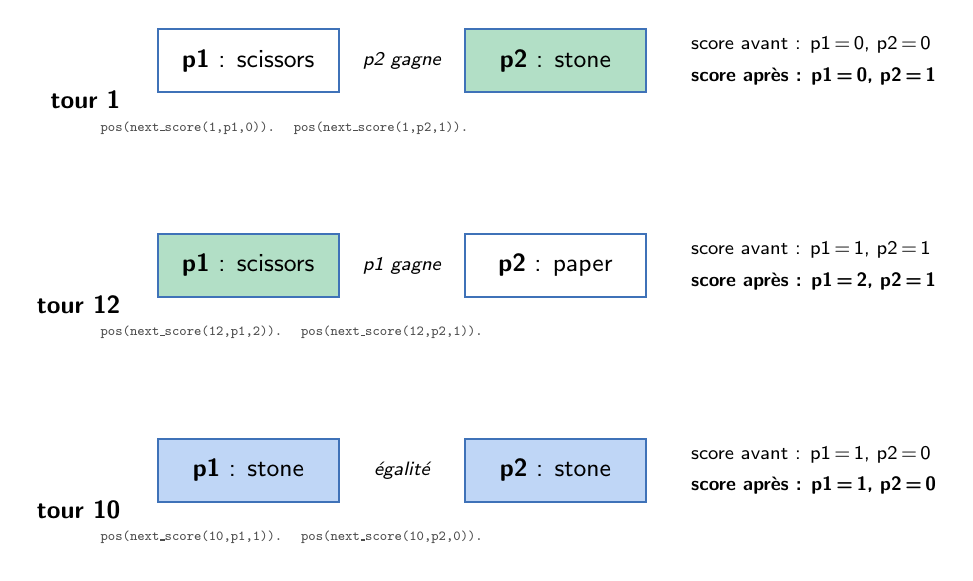
\begin{tikzpicture}[x=1cm,y=1cm]
\node[anchor=east,font=\small\bfseries] at (1.5,-0.00) {tour 1};
\node[draw=marine,fill=white,minimum width=2.3cm,minimum height=0.8cm,line width=0.8pt,font=\small] at (3.0,0.50) {\textbf{p1} : scissors};
\node[draw=marine,fill=vert!35,minimum width=2.3cm,minimum height=0.8cm,line width=0.8pt,font=\small] at (6.9,0.50) {\textbf{p2} : stone};
\node[font=\scriptsize\itshape] at (4.95,0.50) {p2 gagne};
\node[anchor=west,font=\scriptsize] at (8.5,0.70) {score avant : p1\,=\,0, p2\,=\,0};
\node[anchor=west,font=\scriptsize\bfseries] at (8.5,0.30) {score après : p1\,=\,0, p2\,=\,1};
\node[anchor=west,font=\tiny\ttfamily,text=encre!80] at (1.0,-0.35) {pos(next\_score(1,p1,0)).\; pos(next\_score(1,p2,1)).};
\node[anchor=east,font=\small\bfseries] at (1.5,-2.60) {tour 12};
\node[draw=marine,fill=vert!35,minimum width=2.3cm,minimum height=0.8cm,line width=0.8pt,font=\small] at (3.0,-2.10) {\textbf{p1} : scissors};
\node[draw=marine,fill=white,minimum width=2.3cm,minimum height=0.8cm,line width=0.8pt,font=\small] at (6.9,-2.10) {\textbf{p2} : paper};
\node[font=\scriptsize\itshape] at (4.95,-2.10) {p1 gagne};
\node[anchor=west,font=\scriptsize] at (8.5,-1.90) {score avant : p1\,=\,1, p2\,=\,1};
\node[anchor=west,font=\scriptsize\bfseries] at (8.5,-2.30) {score après : p1\,=\,2, p2\,=\,1};
\node[anchor=west,font=\tiny\ttfamily,text=encre!80] at (1.0,-2.95) {pos(next\_score(12,p1,2)).\; pos(next\_score(12,p2,1)).};
\node[anchor=east,font=\small\bfseries] at (1.5,-5.20) {tour 10};
\node[draw=marine,fill=pastel,minimum width=2.3cm,minimum height=0.8cm,line width=0.8pt,font=\small] at (3.0,-4.70) {\textbf{p1} : stone};
\node[draw=marine,fill=pastel,minimum width=2.3cm,minimum height=0.8cm,line width=0.8pt,font=\small] at (6.9,-4.70) {\textbf{p2} : stone};
\node[font=\scriptsize\itshape] at (4.95,-4.70) {égalité};
\node[anchor=west,font=\scriptsize] at (8.5,-4.50) {score avant : p1\,=\,1, p2\,=\,0};
\node[anchor=west,font=\scriptsize\bfseries] at (8.5,-4.90) {score après : p1\,=\,1, p2\,=\,0};
\node[anchor=west,font=\tiny\ttfamily,text=encre!80] at (1.0,-5.55) {pos(next\_score(10,p1,1)).\; pos(next\_score(10,p2,0)).};
\end{tikzpicture}
\end{center}
\textbf{Comment lire :}
\begin{itemize}
  \item \textbf{tour 1} : \texttt{scissors} contre \texttt{stone}, p2 gagne. Scores $0,0 \to 0,1$.
  \item \textbf{tour 12} : \texttt{scissors} contre \texttt{paper}, p1 gagne. Scores $1,1 \to 2,1$.
  \item \textbf{tour 10} : \texttt{stone} contre \texttt{stone}, égalité. Scores inchangés ($1,0 \to 1,0$).
\end{itemize}
Les négatifs du tour 1 sont toutes les autres valeurs : \texttt{neg(next\_score(1,p1,1))}, \texttt{neg(next\_score(1,p1,2))}, \texttt{neg(next\_score(1,p1,3))}, \texttt{neg(next\_score(1,p2,0))}\ldots

\titrebox{5}{The learned program (le programme appris)}
Le commentaire en tête de \texttt{bias.pl} donne le meilleur programme (3 clauses) :
\begin{moi}\small
\texttt{next\_score(A,B,C) :- my\_true\_score(A,B,D), my\_succ(D,C), wins(A,B).}\\
\texttt{next\_score(A,B,C) :- wins(A,D), my\_true\_score(A,B,C), different(B,D).}\\
\texttt{next\_score(A,B,C) :- does(A,D,E), my\_true\_score(A,B,C), different(B,D), does(A,B,E).}
\end{moi}
\renewcommand{\arraystretch}{1.3}
\begin{tabular}{@{}c L{6.4cm}L{7.4cm}@{}}
\textbf{Clause} & \textbf{En français} & \textbf{Cas du jeu}\\\hline
1 & si \texttt{B} gagne le tour \texttt{A}, son nouveau score \texttt{C} est son score \texttt{D} plus un (\texttt{my\_succ}) & \texttt{B} \textbf{gagne} (tour 12, p1)\\
2 & si l'autre joueur \texttt{D} gagne, le score de \texttt{B} ne change pas & \texttt{B} \textbf{perd} (tour 1, p1)\\
3 & si \texttt{B} et un autre joueur \texttt{D} jouent la même action \texttt{E}, le score ne change pas & \textbf{égalité} (tour 10)\\
\end{tabular}
\ce{trois clauses, trois issues possibles d'un tour : gagner, perdre, égalité. La clause 1 est la seule qui change le score ; elle utilise \texttt{wins}, donc une règle de $\mathcal{R}$.}
\textbf{Résultat annoncé :} TP\,=\,108, FN\,=\,0, TN\,=\,356, FP\,=\,0, soit (ALL, NONE). J'ai recalculé : sur les 54 tours qui ont des faits \texttt{does}, le programme couvre les 108 positifs et aucun des 324 négatifs ; les 32 négatifs des tours 2, 5, 8 et 14 ne sont couverts par rien (pas de \texttt{does}), ce qui donne bien 356 vrais négatifs.
Le fichier indique aussi 1607 programmes testés, \texttt{max\_clauses(4)}, \texttt{max\_vars(5)}, \texttt{max\_body(7)}.

\titrebox{6}{Points de vigilance pour la preuve federated}
\begin{piege}
\textbf{Les parties \texttt{iggp-rps\_part1/2/3} ne séparent pas les faits.} Je les ai ouvertes : chacune contient dans son \texttt{bk.pl} \emph{tous} les faits \texttt{does} (54 tours) et \texttt{my\_true\_score} (58 tours). Ce sont les \emph{exemples} qui sont répartis (155, 155 et 154 lignes, sans doublon), mais les mêmes tours apparaissent chez les trois clients. Donc $\mathcal{B}_i=\mathcal{B}$ : la Knowledge Locality est vraie trivialement, mais aucune connaissance n'est privée.
\end{piege}
\begin{piege}
\textbf{A2 ne tient pas à la lettre} : les constantes \texttt{p1}, \texttt{p2}, \texttt{stone}, \texttt{paper}, \texttt{scissors} sont partagées par tous les tours, et les numéros de tour (1 à 58) utilisent les mêmes entiers que les scores (0 à 3). Les \emph{types} (\texttt{ex}, \texttt{player}, \texttt{action}, \texttt{int}) les séparent dans le biais, mais la preuve de la Part~I raisonne sans types. Même remarque que pour Zendo.
\end{piege}
\begin{piege}
\textbf{La garde de localité est commentée.} Dans \texttt{bias.pl}, la contrainte ``une seule variable de type \texttt{ex} par clause'' (présente dans Zendo, Mutagenesis et Carcinogenesis) est écrite avec la mention \texttt{HACK BECAUSE WE DO NOT LEARN FROM INTERPRETATIONS}, mais \textbf{en commentaire}. Rien n'empêche donc un programme de mélanger deux tours différents.
\end{piege}
\ce{pour une expérience où chaque client ne voit que \emph{ses} tours, il faudrait répartir les faits \texttt{does} et \texttt{my\_true\_score} par tour (comme Trains répartit par train), en gardant \texttt{beats}, \texttt{my\_succ}, \texttt{player}, \texttt{different} et les trois règles dans $\mathcal{R}$.}

% =====================================================================
%  ANNEXE : Mutagenesis
% =====================================================================
\partie{VII}{Annexe : le dataset Mutagenesis}{Des molécules décrites atome par atome. Schéma des données, deux molécules dessinées, les règles $\mathcal{R}$ du BK, ce que le biais autorise, et les points de vigilance pour la preuve.}

\titrebox{1}{The task (la tâche)}
On a 230 composés chimiques (des \EN{nitroaromatics}{composés nitro-aromatiques}). Chacun est soit \emph{mutagène} (il peut modifier l'ADN), soit non mutagène. Le prédicat à apprendre est \texttt{active(D)} : ``le composé \texttt{D} est actif (mutagène)''.
\begin{moi}
138 \EN{positive examples}{positifs} et 92 \EN{negative examples}{négatifs}. Exemple : \texttt{pos(active(d18)).}\quad \texttt{neg(active(d5)).}
\end{moi}
\textbf{Taille du BK :} 5894 atomes (\texttt{atm}) et 6309 liaisons (\texttt{bond}), de 13 à 40 atomes par molécule. Les 230 composés ont tous au moins un groupe \texttt{nitro} dans le BK, donc \texttt{nitro} seul ne sépare rien (138 positifs et 92 négatifs en ont).
Le benchmark vient de la littérature d'ILP sur la mutagénicité (Srinivasan, King et al.) : à citer, vérifier la référence exacte.

\titrebox{2}{The schema (le schéma) : composé, atomes, liaisons}
\begin{center}
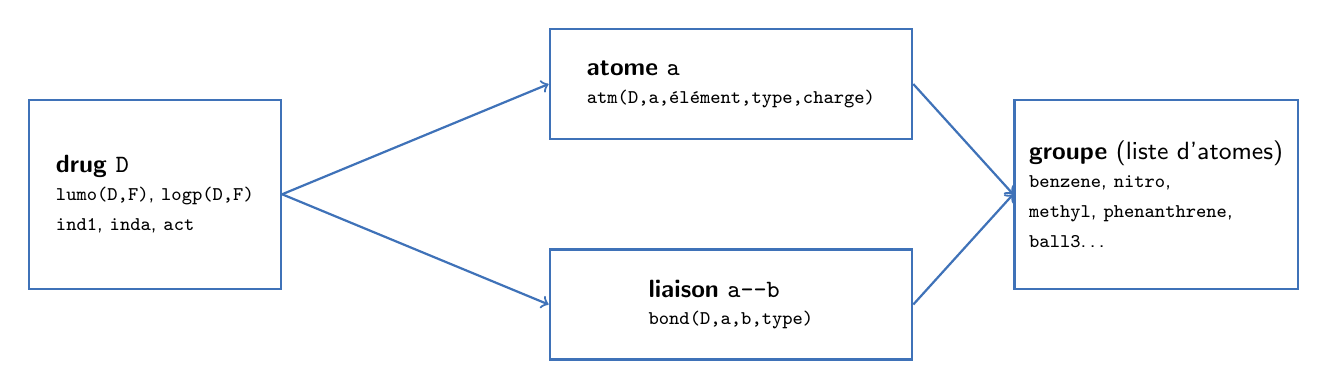
\begin{tikzpicture}[x=1cm,y=1cm, every node/.style={font=\small}]
  \node[draw=marine,fill=white,line width=0.9pt,minimum width=3.2cm,minimum height=2.4cm,align=left] (D) at (0,0) {\textbf{drug} \texttt{D}\\[-1pt]\scriptsize \texttt{lumo(D,F)}, \texttt{logp(D,F)}\\ \scriptsize \texttt{ind1}, \texttt{inda}, \texttt{act}};
  \node[draw=marine,fill=white,line width=0.9pt,minimum width=4.6cm,minimum height=1.4cm,align=left,anchor=west] (A) at (5.0,1.4) {\textbf{atome} \texttt{a}\\[-1pt]\scriptsize \texttt{atm(D,a,élément,type,charge)}};
  \node[draw=marine,fill=white,line width=0.9pt,minimum width=4.6cm,minimum height=1.4cm,align=left,anchor=west] (B) at (5.0,-1.4) {\textbf{liaison} \texttt{a--b}\\[-1pt]\scriptsize \texttt{bond(D,a,b,type)}};
  \node[draw=marine,fill=white,line width=0.9pt,minimum width=3.6cm,minimum height=2.4cm,align=left,anchor=west] (G) at (10.9,0) {\textbf{groupe} (liste d'atomes)\\[-1pt]\scriptsize \texttt{benzene}, \texttt{nitro},\\ \scriptsize \texttt{methyl}, \texttt{phenanthrene},\\ \scriptsize \texttt{ball3}\ldots};
  \draw[->,thick,marine] (D.east) -- (A.west);
  \draw[->,thick,marine] (D.east) -- (B.west);
  \draw[->,thick,marine] (A.east) -- (G.west);
  \draw[->,thick,marine] (B.east) -- (G.west);
\end{tikzpicture}
\end{center}
\ce{un composé a des atomes (élément comme \texttt{c}, \texttt{h}, \texttt{o}, \texttt{n}, un code de type numérique, une charge partielle) et des liaisons entre atomes (type 1, 2 ou 7). Les groupes chimiques (\texttt{benzene}, \texttt{nitro}\ldots) sont des \emph{listes d'atomes}, calculées à l'avance. \texttt{lumo} et \texttt{logp} sont des mesures par composé.}

\st{Deux molécules dessinées (un atome = un rond)}
Gris = carbone, blanc = hydrogène, rouge = oxygène, bleu = azote, vert = chlore ou fluor. Trait simple = liaison de type 1, double trait = type 2, trait pointillé = type 7 (liaisons des cycles aromatiques : codage du dataset, à confirmer).
La disposition est calculée automatiquement (elle ne reflète pas la vraie géométrie).
\begin{center}
\begin{minipage}[t]{0.49\textwidth}\centering
{\large\bfseries\textcolor{marine}{f1 (positif, 13 atomes)}}\par\vspace{3pt}
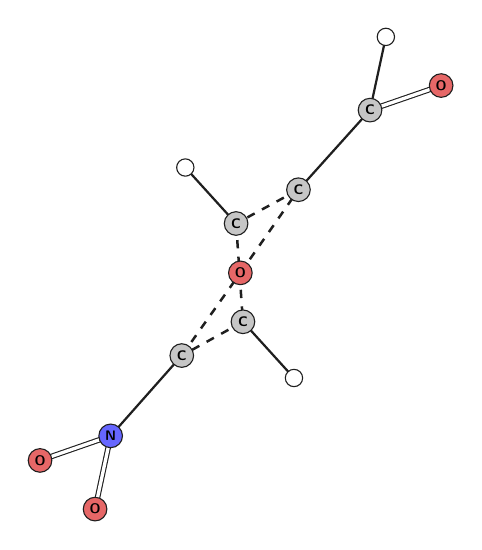
\begin{tikzpicture}[x=3.00cm,y=3.00cm]
\draw[dashed,line width=0.9pt,encre] (0.247,0.352) -- (-0.017,0.209);
\draw[dashed,line width=0.9pt,encre] (-0.017,0.209) -- (0.012,-0.207);
\draw[dashed,line width=0.9pt,encre] (0.012,-0.207) -- (-0.247,-0.350);
\draw[dashed,line width=0.9pt,encre] (-0.247,-0.350) -- (0.001,-0.000);
\draw[dashed,line width=0.9pt,encre] (0.001,-0.000) -- (0.247,0.352);
\draw[line width=0.8pt,encre] (-0.017,0.209) -- (-0.232,0.446);
\draw[line width=0.8pt,encre] (0.012,-0.207) -- (0.228,-0.445);
\draw[line width=0.8pt,encre] (-0.247,-0.350) -- (-0.548,-0.690);
\draw[double distance=1.2pt,line width=0.4pt,encre] (-0.548,-0.690) -- (-0.847,-0.794);
\draw[double distance=1.2pt,line width=0.4pt,encre] (-0.548,-0.690) -- (-0.614,-1.000);
\draw[line width=0.8pt,encre] (0.247,0.352) -- (0.550,0.689);
\draw[double distance=1.2pt,line width=0.4pt,encre] (0.550,0.689) -- (0.851,0.793);
\draw[line width=0.8pt,encre] (0.550,0.689) -- (0.617,0.999);
\node[circle,draw=encre,fill=gray!45,inner sep=0pt,minimum size=0.30cm,font=\tiny\bfseries,line width=0.4pt] at (0.247,0.352) {C};
\node[circle,draw=encre,fill=gray!45,inner sep=0pt,minimum size=0.30cm,font=\tiny\bfseries,line width=0.4pt] at (-0.017,0.209) {C};
\node[circle,draw=encre,fill=gray!45,inner sep=0pt,minimum size=0.30cm,font=\tiny\bfseries,line width=0.4pt] at (0.012,-0.207) {C};
\node[circle,draw=encre,fill=gray!45,inner sep=0pt,minimum size=0.30cm,font=\tiny\bfseries,line width=0.4pt] at (-0.247,-0.350) {C};
\node[circle,draw=encre,fill=rouge!70,inner sep=0pt,minimum size=0.30cm,font=\tiny\bfseries,line width=0.4pt] at (0.001,-0.000) {O};
\node[circle,draw=encre,fill=white,inner sep=0pt,minimum size=0.22cm,font=\tiny\bfseries,line width=0.4pt] at (-0.232,0.446) {};
\node[circle,draw=encre,fill=white,inner sep=0pt,minimum size=0.22cm,font=\tiny\bfseries,line width=0.4pt] at (0.228,-0.445) {};
\node[circle,draw=encre,fill=blue!60,inner sep=0pt,minimum size=0.30cm,font=\tiny\bfseries,line width=0.4pt] at (-0.548,-0.690) {N};
\node[circle,draw=encre,fill=rouge!70,inner sep=0pt,minimum size=0.30cm,font=\tiny\bfseries,line width=0.4pt] at (-0.847,-0.794) {O};
\node[circle,draw=encre,fill=rouge!70,inner sep=0pt,minimum size=0.30cm,font=\tiny\bfseries,line width=0.4pt] at (-0.614,-1.000) {O};
\node[circle,draw=encre,fill=gray!45,inner sep=0pt,minimum size=0.30cm,font=\tiny\bfseries,line width=0.4pt] at (0.550,0.689) {C};
\node[circle,draw=encre,fill=rouge!70,inner sep=0pt,minimum size=0.30cm,font=\tiny\bfseries,line width=0.4pt] at (0.851,0.793) {O};
\node[circle,draw=encre,fill=white,inner sep=0pt,minimum size=0.22cm,font=\tiny\bfseries,line width=0.4pt] at (0.617,0.999) {};
\end{tikzpicture}
\end{minipage}\hfill
\begin{minipage}[t]{0.49\textwidth}\centering
{\large\bfseries\textcolor{rouge}{d116 (négatif, 14 atomes)}}\par\vspace{3pt}
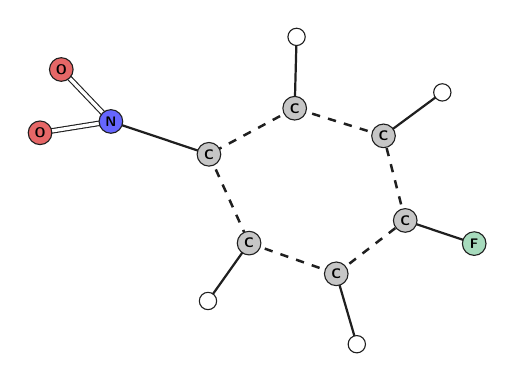
\begin{tikzpicture}[x=3.00cm,y=3.00cm]
\draw[dashed,line width=0.9pt,encre] (0.254,-0.410) -- (0.546,-0.184);
\draw[dashed,line width=0.9pt,encre] (0.546,-0.184) -- (0.454,0.174);
\draw[dashed,line width=0.9pt,encre] (0.454,0.174) -- (0.078,0.291);
\draw[dashed,line width=0.9pt,encre] (0.078,0.291) -- (-0.285,0.096);
\draw[dashed,line width=0.9pt,encre] (-0.285,0.096) -- (-0.115,-0.280);
\draw[dashed,line width=0.9pt,encre] (-0.115,-0.280) -- (0.254,-0.410);
\draw[line width=0.8pt,encre] (0.254,-0.410) -- (0.341,-0.708);
\draw[line width=0.8pt,encre] (0.454,0.174) -- (0.703,0.358);
\draw[line width=0.8pt,encre] (0.078,0.291) -- (0.086,0.593);
\draw[line width=0.8pt,encre] (-0.115,-0.280) -- (-0.289,-0.525);
\draw[line width=0.8pt,encre] (-0.285,0.096) -- (-0.700,0.235);
\draw[line width=0.8pt,encre] (0.546,-0.184) -- (0.838,-0.282);
\draw[double distance=1.2pt,line width=0.4pt,encre] (-0.700,0.235) -- (-0.910,0.455);
\draw[double distance=1.2pt,line width=0.4pt,encre] (-0.700,0.235) -- (-1.000,0.187);
\node[circle,draw=encre,fill=gray!45,inner sep=0pt,minimum size=0.30cm,font=\tiny\bfseries,line width=0.4pt] at (0.254,-0.410) {C};
\node[circle,draw=encre,fill=gray!45,inner sep=0pt,minimum size=0.30cm,font=\tiny\bfseries,line width=0.4pt] at (0.546,-0.184) {C};
\node[circle,draw=encre,fill=gray!45,inner sep=0pt,minimum size=0.30cm,font=\tiny\bfseries,line width=0.4pt] at (0.454,0.174) {C};
\node[circle,draw=encre,fill=gray!45,inner sep=0pt,minimum size=0.30cm,font=\tiny\bfseries,line width=0.4pt] at (0.078,0.291) {C};
\node[circle,draw=encre,fill=gray!45,inner sep=0pt,minimum size=0.30cm,font=\tiny\bfseries,line width=0.4pt] at (-0.285,0.096) {C};
\node[circle,draw=encre,fill=gray!45,inner sep=0pt,minimum size=0.30cm,font=\tiny\bfseries,line width=0.4pt] at (-0.115,-0.280) {C};
\node[circle,draw=encre,fill=white,inner sep=0pt,minimum size=0.22cm,font=\tiny\bfseries,line width=0.4pt] at (0.341,-0.708) {};
\node[circle,draw=encre,fill=white,inner sep=0pt,minimum size=0.22cm,font=\tiny\bfseries,line width=0.4pt] at (0.703,0.358) {};
\node[circle,draw=encre,fill=white,inner sep=0pt,minimum size=0.22cm,font=\tiny\bfseries,line width=0.4pt] at (0.086,0.593) {};
\node[circle,draw=encre,fill=white,inner sep=0pt,minimum size=0.22cm,font=\tiny\bfseries,line width=0.4pt] at (-0.289,-0.525) {};
\node[circle,draw=encre,fill=blue!60,inner sep=0pt,minimum size=0.30cm,font=\tiny\bfseries,line width=0.4pt] at (-0.700,0.235) {N};
\node[circle,draw=encre,fill=vert!40,inner sep=0pt,minimum size=0.30cm,font=\tiny\bfseries,line width=0.4pt] at (0.838,-0.282) {F};
\node[circle,draw=encre,fill=rouge!70,inner sep=0pt,minimum size=0.30cm,font=\tiny\bfseries,line width=0.4pt] at (-0.910,0.455) {O};
\node[circle,draw=encre,fill=rouge!70,inner sep=0pt,minimum size=0.30cm,font=\tiny\bfseries,line width=0.4pt] at (-1.000,0.187) {O};
\end{tikzpicture}
\end{minipage}
\end{center}

\titrebox{3}{The rules $\mathcal{R}$ of the background knowledge (les règles du BK)}
Oui : le \texttt{bk.pl} contient des règles (12 clauses, hors directives \texttt{style\_check}). Aucune ne parle de chimie : ce sont des \textbf{règles utilitaires et de typage}.
\renewcommand{\arraystretch}{1.25}
\begin{tabular}{@{}L{4.2cm}L{12.2cm}@{}}
\textbf{Règle} & \textbf{Rôle}\\\hline
\texttt{drug(D)}, \texttt{atomid(A)} & types : \texttt{D} est un nom de la forme lettre + nombre de 1 à 230 ; \texttt{A} est un identifiant d'atome de la forme \texttt{d12\_3}. Elles utilisent \texttt{name/2}, des bornes (230, 500) et le code de caractère \texttt{\_} (95)\\
\texttt{charge}, \texttt{energy}, \texttt{hydrophob} & types : \texttt{X} est un flottant\\
\texttt{ring}, \texttt{ringlist} & types : le nom commence par la lettre \texttt{r} (code 114)\\
\texttt{append/3} & concaténation de listes (règle récursive, 2 clauses)\\
\texttt{gteq/2}, \texttt{lteq/2} & comparaisons ``$\ge$'' et ``$\le$'' entre flottants (2 clauses chacun)\\
\end{tabular}
\ce{ces règles ne contiennent aucune constante propre à un composé. Elles contiennent seulement des bornes numériques (1 à 230, 500) et des codes de caractère, identiques pour tous les clients. Elles sont dans $\mathcal{R}$ de la preuve.}

\st{Ce que Popper a le droit d'utiliser (\texttt{bias.pl})}
Le biais autorise 19 prédicats dans le corps (\texttt{lumo}, \texttt{logp}, \texttt{bond}, \texttt{atm}, \texttt{gteq}, \texttt{lteq}, les groupes chimiques, \texttt{member}\ldots), ainsi que \texttt{ind1}, \texttt{inda}, \texttt{act} et \texttt{zero}, et les neuf éléments chimiques comme constantes. Limites : \texttt{max\_clauses(6)}, \texttt{max\_vars(5)}, \texttt{max\_body(6)}. Les directions sont déclarées pour tous les prédicats, avec plusieurs directions pour \texttt{bond} (\texttt{(in,out,out,out)} ou \texttt{(in,in,out,out)}) et \texttt{ball3}.
\begin{moi}
\textbf{Garde de localité dans le biais :} \texttt{:- clause(C), \#count\{V : clause\_var(C,V), var\_type(C,V,drug)\} != 1.}\\
Chaque clause doit contenir \textbf{exactement une variable de type \texttt{drug}} : celle de la tête. Tous les littéraux qui lisent un atome ou une liaison parlent donc \emph{du composé de l'exemple}.
\end{moi}

\titrebox{4}{Que sait-on de la règle à apprendre ?}
Contrairement à Trains, \textbf{aucun programme final n'est documenté} dans les fichiers (pas de commentaire de solution dans le \texttt{bias.pl}), et je n'ai pas lancé Popper. Ce que j'ai mesuré sur les données :
\renewcommand{\arraystretch}{1.25}
\begin{center}
\begin{tabular}{@{}L{7.6cm}c c@{}}
\textbf{Propriété} & \textbf{positifs (138)} & \textbf{négatifs (92)}\\\hline
\texttt{ind1 = 1} (indicateur) & 103 & 17\\
\texttt{inda = 1} (indicateur) & 5 & 0\\
possède un groupe \texttt{phenanthrene} & 30 & 4\\
possède un groupe \texttt{ball3} & 31 & 2\\
possède un groupe \texttt{methyl} & 7 & 21\\
\texttt{lumo} moyen & $-1{,}87$ & $-1{,}34$\\
\texttt{logp} moyen & 3,86 & 2,71\\
\end{tabular}
\end{center}
Aucune propriété seule ne sépare les deux classes : il faut combiner plusieurs conditions (donc plusieurs clauses, d'où \texttt{max\_clauses(6)}).
\begin{piege}
\textbf{Attention à \texttt{act}.} \texttt{act(D,F)} est l'activité mesurée du composé. Je l'ai vérifié : les 138 positifs ont tous \texttt{act} $>0$ (minimum $0{,}03$) et les 92 négatifs ont tous \texttt{act} $\le0$. Une règle ``\texttt{act} positif'' séparerait donc \emph{parfaitement} les classes. La direction déclarée est \texttt{act(out,in)} : le flottant est une \emph{entrée}, il ne peut pas être lu en sortie, ce qui limite l'usage. Mais \texttt{act} reste dans le biais : à vérifier avant d'interpréter un résultat.
\end{piege}

\titrebox{5}{Points de vigilance pour la preuve federated}
\begin{itemize}
  \item \textbf{A1 Example Locality :} la partition \texttt{iid\_3\_seed\_42} répartit les exemples (77, 77 et 76 composés), et chaque exemple a ses faits \texttt{atm} dans son client. \emph{Respectée.}
  \item \textbf{A2 Separated Local Constants :} les identifiants d'atomes sont préfixés par le composé (\texttt{d12\_3}), donc locaux. Mais deux écarts : \textbf{33 composés ont leurs faits dans les trois clients à la fois} (chaque client voit environ 100 composés pour 77 exemples), et les constantes chimiques (\texttt{c}, \texttt{h}, \texttt{o}\ldots, codes de type, charges) sont partagées. À vérifier.
  \item \textbf{A3 Directions :} déclarées. En plus, la garde ``une seule variable \texttt{drug}'' joue le rôle de \emph{garde de localité} : sans elle, un littéral comme \texttt{ind1(B,1.0)} avec \texttt{B} libre parcourrait les faits de tous les composés. Cette garde n'apparaît pas dans l'énoncé de A3 de la Part~I : \textbf{à ajouter comme condition du biais}.
\end{itemize}

% =====================================================================
%  ANNEXE : Carcinogenesis
% =====================================================================
\partie{VIII}{Annexe : le dataset Carcinogenesis}{Même format que Mutagenesis, mais avec beaucoup plus de règles dans le BK (dont 28 clauses \texttt{mutagenic/1}) et des résultats d'expériences biologiques.}

\titrebox{1}{The task (la tâche)}
On a 298 composés (162 positifs, 136 négatifs). Le prédicat à apprendre est \texttt{active(D)} : ``\texttt{D} est actif'', c'est-à-dire cancérogène dans les tests animaux (\emph{carcinogenic activity}). Source : benchmark ILP de cancérogénicité (Srinivasan, King et al.), à citer après vérification.
\begin{moi}
\texttt{pos(active(d107)).}\quad \texttt{pos(active(d284)).}\quad \ldots\quad 162 positifs et 136 négatifs.
\end{moi}
\textbf{Taille du BK :} 9205 atomes (\texttt{atm}), 9319 liaisons (\texttt{bond}), 340 composés déclarés (\texttt{drug/1}), dont 42 sans exemple.

\titrebox{2}{The schema (le schéma)}
\begin{center}
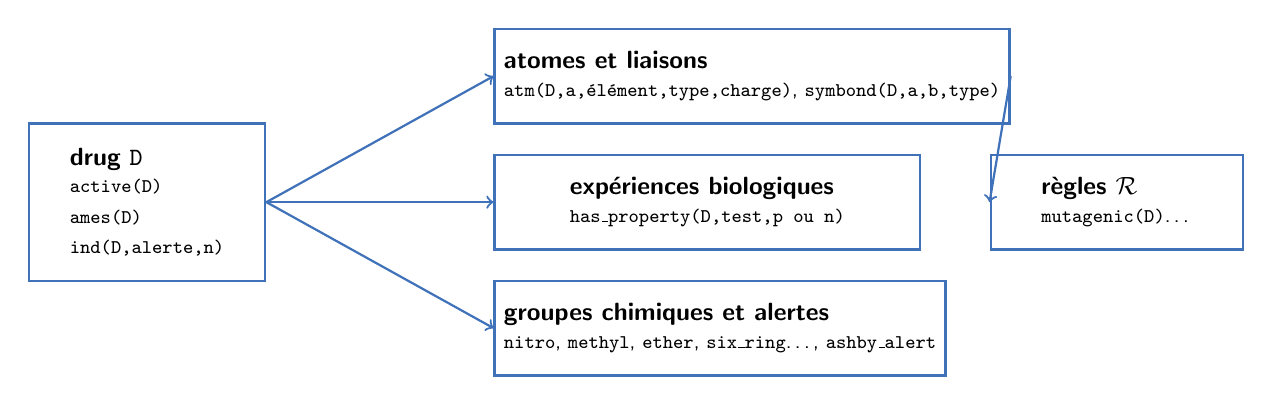
\begin{tikzpicture}[x=1cm,y=1cm, every node/.style={font=\small}]
  \node[draw=marine,fill=white,line width=0.9pt,minimum width=3.0cm,minimum height=2.0cm,align=left] (D) at (0,0) {\textbf{drug} \texttt{D}\\[-1pt]\scriptsize \texttt{active(D)}\\ \scriptsize \texttt{ames(D)}\\ \scriptsize \texttt{ind(D,alerte,n)}};
  \node[draw=marine,fill=white,line width=0.9pt,minimum width=5.4cm,minimum height=1.2cm,align=left,anchor=west] (A) at (4.4,1.6) {\textbf{atomes et liaisons}\\[-1pt]\scriptsize \texttt{atm(D,a,élément,type,charge)}, \texttt{symbond(D,a,b,type)}};
  \node[draw=marine,fill=white,line width=0.9pt,minimum width=5.4cm,minimum height=1.2cm,align=left,anchor=west] (P) at (4.4,0) {\textbf{expériences biologiques}\\[-1pt]\scriptsize \texttt{has\_property(D,test,p ou n)}};
  \node[draw=marine,fill=white,line width=0.9pt,minimum width=5.4cm,minimum height=1.2cm,align=left,anchor=west] (G) at (4.4,-1.6) {\textbf{groupes chimiques et alertes}\\[-1pt]\scriptsize \texttt{nitro}, \texttt{methyl}, \texttt{ether}, \texttt{six\_ring}\ldots, \texttt{ashby\_alert}};
  \node[draw=marine,fill=white,line width=0.9pt,minimum width=3.2cm,minimum height=1.2cm,align=left,anchor=west] (R) at (10.7,0) {\textbf{règles $\mathcal{R}$}\\[-1pt]\scriptsize \texttt{mutagenic(D)}\ldots};
  \draw[->,thick,marine] (D.east) -- (A.west);
  \draw[->,thick,marine] (D.east) -- (P.west);
  \draw[->,thick,marine] (D.east) -- (G.west);
  \draw[->,thick,marine] (A.east) -- (R.west);
\end{tikzpicture}
\end{center}
\renewcommand{\arraystretch}{1.25}
\begin{tabular}{@{}L{4.6cm}L{11.8cm}@{}}
\textbf{Prédicat} & \textbf{Contenu (comptes dans \texttt{bk.pl})}\\\hline
\texttt{has\_property} (1319) & résultats de 13 tests (\texttt{salmonella}, \texttt{cytogen\_ca}, \texttt{cytogen\_sce}, \texttt{mouse\_lymph}, \texttt{chromaberr}\ldots) avec valeur \texttt{p} (positif) ou \texttt{n} (négatif)\\
\texttt{ames} (142) & composés pour lesquels le test d'Ames (mutagénicité) est positif\\
\texttt{ashby\_alert} (748), \texttt{ind} (394) & alertes structurales (28 types : \texttt{nitro}, \texttt{amino}\ldots) et nombre d'alertes d'un composé\\
groupes (\texttt{six\_ring}, \texttt{methyl}, \texttt{ether}\ldots) & listes d'atomes pour chaque motif chimique\\
\end{tabular}

\st{Deux molécules dessinées (mêmes conventions que Mutagenesis)}
Les éléments (symboles) viennent des données. \texttt{d274} est un composé \emph{positif} de 5 atomes, \texttt{d178} un composé \emph{négatif} de 3 atomes (titane et deux oxygènes).
\begin{center}
\begin{minipage}[t]{0.49\textwidth}\centering
{\large\bfseries\textcolor{marine}{d274 (positif, 5 atomes)}}\par\vspace{3pt}
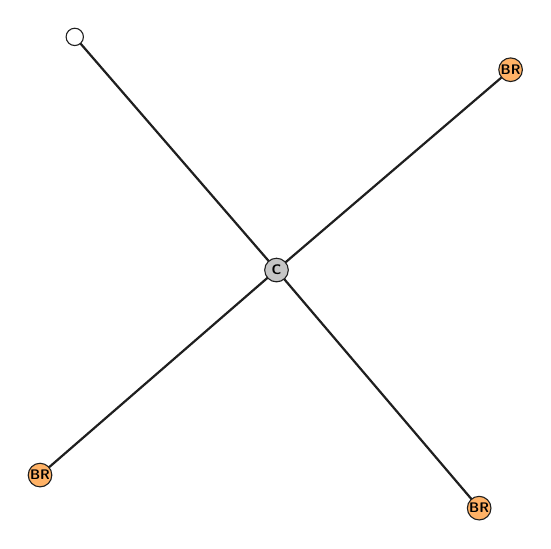
\begin{tikzpicture}[x=3.00cm,y=3.00cm]
\draw[line width=0.8pt,encre] (0.001,0.008) -- (-1.000,-0.860);
\draw[line width=0.8pt,encre] (0.001,0.008) -- (0.992,0.856);
\draw[line width=0.8pt,encre] (0.001,0.008) -- (0.859,-1.000);
\draw[line width=0.8pt,encre] (0.001,0.008) -- (-0.853,0.995);
\node[circle,draw=encre,fill=gray!45,inner sep=0pt,minimum size=0.30cm,font=\tiny\bfseries,line width=0.4pt] at (0.001,0.008) {C};
\node[circle,draw=encre,fill=orange!60,inner sep=0pt,minimum size=0.30cm,font=\tiny\bfseries,line width=0.4pt] at (-1.000,-0.860) {BR};
\node[circle,draw=encre,fill=orange!60,inner sep=0pt,minimum size=0.30cm,font=\tiny\bfseries,line width=0.4pt] at (0.992,0.856) {BR};
\node[circle,draw=encre,fill=orange!60,inner sep=0pt,minimum size=0.30cm,font=\tiny\bfseries,line width=0.4pt] at (0.859,-1.000) {BR};
\node[circle,draw=encre,fill=white,inner sep=0pt,minimum size=0.22cm,font=\tiny\bfseries,line width=0.4pt] at (-0.853,0.995) {};
\end{tikzpicture}
\end{minipage}\hfill
\begin{minipage}[t]{0.49\textwidth}\centering
{\large\bfseries\textcolor{rouge}{d178 (négatif, 3 atomes)}}\par\vspace{3pt}
\begin{tikzpicture}[x=3.00cm,y=3.00cm]
\draw[double distance=1.2pt,line width=0.4pt,encre] (-0.002,-0.001) -- (-0.998,-0.625);
\draw[double distance=1.2pt,line width=0.4pt,encre] (-0.002,-0.001) -- (1.000,0.626);
\node[circle,draw=encre,fill=white,inner sep=0pt,minimum size=0.30cm,font=\tiny\bfseries,line width=0.4pt] at (-0.002,-0.001) {TI};
\node[circle,draw=encre,fill=rouge!70,inner sep=0pt,minimum size=0.30cm,font=\tiny\bfseries,line width=0.4pt] at (-0.998,-0.625) {O};
\node[circle,draw=encre,fill=rouge!70,inner sep=0pt,minimum size=0.30cm,font=\tiny\bfseries,line width=0.4pt] at (1.000,0.626) {O};
\end{tikzpicture}
\end{minipage}
\end{center}

\titrebox{3}{The rules $\mathcal{R}$ of the background knowledge (les règles du BK)}
Oui, et beaucoup : environ 46 clauses (le générateur en compte 46 ou 47 par client). Deux familles :
\begin{itemize}
  \item \textbf{Utilitaires et typage :} \texttt{eq}, \texttt{atomid}, \texttt{charge}, \texttt{ring}, \texttt{list}, \texttt{element} (appartenance à une liste), \texttt{gteq}, \texttt{lteq}, \texttt{connected} (deux cycles partageant un atome), \texttt{symbond}/\texttt{sym\_bond} (liaison dans les deux sens).
  \item \textbf{Chimie : 28 clauses \texttt{mutagenic/1}} (certaines en doublon). Chacune est un motif structural qui rend un composé \emph{mutagène}.
\end{itemize}
\begin{moi}\small
\texttt{mutagenic(A) :- atm(A,B,c,22,-0.114).}\\
\texttt{mutagenic(A) :- atm(A,B,c,27,C), lteq(C,-0.085).}\\
\texttt{mutagenic(A) :- atm(A,B,o,40,C), atm(A,D,n,32,C).}
\end{moi}
En français : \emph{un composé est mutagène s'il contient un atome de carbone de type 22 et de charge $-0{,}114$}, ou \emph{un carbone de type 27 de charge au plus $-0{,}085$}, ou \emph{un oxygène de type 40 et un azote de type 32 de même charge}, etc.
Ces motifs semblent issus d'un apprentissage préalable sur la mutagénicité (d'où le lien avec Mutagenesis) : \emph{hypothèse de ma part, à vérifier}. Popper peut appeler \texttt{mutagenic(D)} comme un prédicat : la règle est déjà écrite.
\ce{ces règles lisent \texttt{atm(A,\ldots)} avec \texttt{A} la variable du composé de la tête. Elles ne contiennent que des constantes chimiques (éléments, codes de type, charges), aucun identifiant de composé : conforme à A2 pour $\mathcal{R}$.}

\titrebox{4}{Que sait-on de la règle à apprendre ?}
Comme pour Mutagenesis, \textbf{aucun programme final n'est documenté}, et je n'ai pas lancé Popper. Mesures sur les données :
\renewcommand{\arraystretch}{1.25}
\begin{center}
\begin{tabular}{@{}L{8.4cm}c c@{}}
\textbf{Propriété} & \textbf{positifs (162)} & \textbf{négatifs (136)}\\\hline
test d'Ames positif (\texttt{ames(D)}) & 89 & 37\\
\texttt{salmonella} positif & 78 & 33\\
au moins une alerte (\texttt{ind}) & 123 & 83\\
au moins un résultat \texttt{has\_property} & 154 & 126\\
\end{tabular}
\end{center}
\begin{piege}
Les résultats \texttt{ames} et \texttt{salmonella} sont des \emph{tests de mutagénicité} du même composé : très corrélés avec la cancérogénicité. Ils font partie du problème d'origine, mais il faut le savoir pour interpréter les règles apprises (une règle qui s'appuie sur \texttt{ames} ne ``comprend'' pas la structure chimique).
\end{piege}

\titrebox{5}{Points de vigilance pour la preuve federated}
\begin{itemize}
  \item \textbf{Biais :} directions déclarées, avec la même garde ``une seule variable de type \texttt{drug}''. Les prédicats \texttt{ashby\_alert(out,in,out)} ont le composé en position \emph{non-entrée} : la garde est ce qui évite de parcourir les alertes de tous les composés.
  \item \textbf{Partition \texttt{iid\_3\_seed\_42} :} 100, 99 et 99 exemples, tous avec leurs faits \texttt{atm} locaux. Chaque client voit environ 146 composés dans son BK, dont \textbf{49 communs aux trois clients} : A2 n'est pas respectée à la lettre, comme pour Mutagenesis.
  \item \textbf{$\mathcal{R}$ volumineux :} 46 à 47 clauses par client, identiques. À écrire dans la preuve : ``$\mathcal{R}$ ne contient aucune constante locale'' est vrai ici (constantes chimiques seulement), à vérifier clause par clause.
\end{itemize}

% =====================================================================
%  ANNEXE : Alzheimer
% =====================================================================
\partie{IX}{Annexe : les datasets Alzheimer (acetyl, amine, mem, toxic)}{Quatre problèmes sur les mêmes 37 composés : comparer deux composés à la fois. Schéma, exemples, règles du BK (il n'y en a pas), et points de vigilance.}

\titrebox{1}{The task (la tâche) : comparer deux composés}
Les quatre datasets (\texttt{noisy-alzheimer\_acetyl}, \texttt{\_amine}, \texttt{\_mem}, \texttt{\_toxic}) portent sur les mêmes \textbf{37 composés}, des molécules testées contre la maladie d'Alzheimer. La différence est dans la propriété comparée :
\renewcommand{\arraystretch}{1.25}
\begin{center}
\begin{tabular}{@{}l l c c@{}}
\textbf{Dataset} & \textbf{Prédicat à apprendre} & \textbf{positifs} & \textbf{négatifs}\\\hline
\texttt{acetyl} & \texttt{great(X,Y)} & 530 & 530\\
\texttt{amine} & \texttt{great\_ne(X,Y)} & 274 & 274\\
\texttt{mem} & \texttt{great\_rsd(X,Y)} & 256 & 256\\
\texttt{toxic} & \texttt{less\_toxic(X,Y)} & 354 & 354\\
\end{tabular}
\end{center}
Un exemple est donc une \textbf{paire} de composés (\texttt{X}, \texttt{Y}) : ``\texttt{X} est meilleur que \texttt{Y}'' pour la propriété en question. Exemple : \texttt{pos(great(y1,s1)).}
Selon la littérature (King et al.), les propriétés sont : inhibition de l'acétylcholinestérase (\texttt{acetyl}), inhibition de la recapture d'amines (\texttt{amine}), réversion d'un déficit de mémoire (\texttt{mem}) et faible toxicité (\texttt{toxic}). \emph{Cette correspondance entre noms de prédicats et propriétés est de ma part, à vérifier.}
Le préfixe \texttt{noisy} signale du bruit dans les étiquettes ; \textbf{le taux de bruit n'est pas indiqué dans les fichiers}.

\titrebox{2}{The schema (le schéma) : composé, substituants, propriétés}
\begin{center}
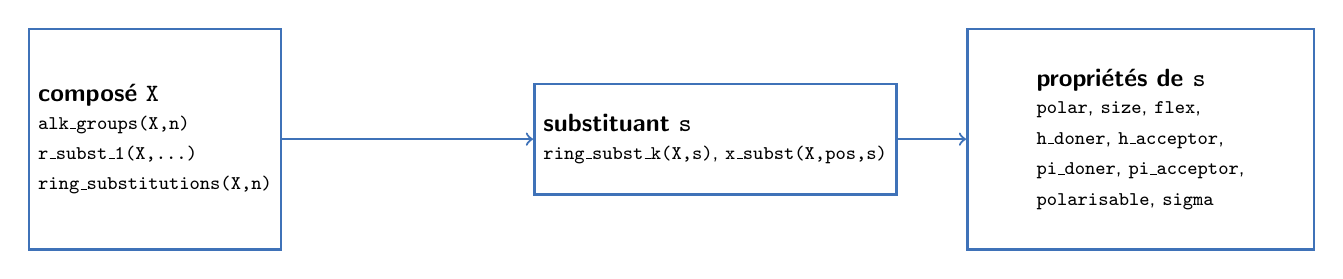
\begin{tikzpicture}[x=1cm,y=1cm, every node/.style={font=\small}]
  \node[draw=marine,fill=white,line width=0.9pt,minimum width=3.2cm,minimum height=2.8cm,align=left] (C) at (0,0) {\textbf{composé} \texttt{X}\\[-1pt]\scriptsize \texttt{alk\_groups(X,n)}\\ \scriptsize \texttt{r\_subst\_1(X,\ldots)}\\ \scriptsize \texttt{ring\_substitutions(X,n)}};
  \node[draw=marine,fill=white,line width=0.9pt,minimum width=4.4cm,minimum height=1.4cm,align=left,anchor=west] (S) at (4.8,0) {\textbf{substituant} \texttt{s}\\[-1pt]\scriptsize \texttt{ring\_subst\_k(X,s)}, \texttt{x\_subst(X,pos,s)}};
  \node[draw=marine,fill=white,line width=0.9pt,minimum width=4.4cm,minimum height=2.8cm,align=left,anchor=west] (P) at (10.3,0) {\textbf{propriétés de \texttt{s}}\\[-1pt]\scriptsize \texttt{polar}, \texttt{size}, \texttt{flex},\\ \scriptsize \texttt{h\_doner}, \texttt{h\_acceptor},\\ \scriptsize \texttt{pi\_doner}, \texttt{pi\_acceptor},\\ \scriptsize \texttt{polarisable}, \texttt{sigma}};
  \draw[->,thick,marine] (C.east) -- (S.west);
  \draw[->,thick,marine] (S.east) -- (P.west);
\end{tikzpicture}
\end{center}
\ce{un composé est décrit par quelques nombres (\texttt{alk\_groups}, \texttt{ring\_substitutions}), un groupe fixé en position R (\texttt{r\_subst\_1}, \texttt{r\_subst\_2}, \texttt{r\_subst\_3}) et les substituants posés sur son cycle (\texttt{ring\_subst\_k}, \texttt{x\_subst}). Chaque substituant (\texttt{ch3}, \texttt{och3}, \texttt{cf3}, \texttt{cl}, \texttt{f}) a des propriétés chimiques.}

\st{Les propriétés des 5 substituants (\texttt{bk.pl})}
\renewcommand{\arraystretch}{1.2}
\begin{center}
\begin{tabular}{@{}l c c c c c c c c@{}}
\textbf{substituant} & polar & size & flex & h\_don & h\_acc & pi\_don & polari & sigma\\\hline
\texttt{ch3} & 0 & 1 & 0 & 0 & 0 & 0 & 1 & 0\\
\texttt{och3} & 2 & 2 & 1 & 0 & 1 & 1 & 1 & 1\\
\texttt{cf3} & 3 & 1 & 0 & 0 & 0 & 0 & 0 & 3\\
\texttt{cl} & 3 & 1 & 0 & 0 & 0 & 0 & 1 & 3\\
\texttt{f} & 5 & 1 & 0 & 0 & 1 & 0 & 0 & 5\\
\end{tabular}
\end{center}
Ces niveaux sont des étiquettes (\texttt{polar0}, \texttt{polar2}\ldots) et le BK contient des tables de comparaison : \texttt{great\_polar(polar2,polar0)} signifie ``\texttt{polar2} est supérieur à \texttt{polar0}'' (45 faits par propriété). \texttt{gt(n,m)} compare des entiers de 0 à 4 (10 faits). Il n'y a \textbf{aucune règle} dans ce BK : tout est dans des faits.

\titrebox{3}{Une paire d'exemples dessinée}
Exemple \texttt{pos(great(y1,s1))} : \texttt{y1} et \texttt{s1} sont identiques (1 groupe alkyle, \texttt{r\_subst\_1 = single\_alk(1)}, \texttt{r\_subst\_2 = aro(1)}, 1 substitution) sauf un substituant en position 4 du cycle :
\begin{center}
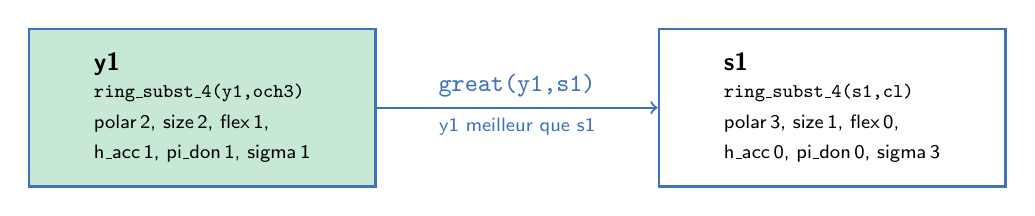
\begin{tikzpicture}[x=1cm,y=1cm, every node/.style={font=\small}]
  \node[draw=marine,fill=vert!25,line width=0.9pt,minimum width=4.4cm,minimum height=2.0cm,align=left] (Y) at (0,0) {\textbf{y1}\\[-1pt]\scriptsize \texttt{ring\_subst\_4(y1,och3)}\\ \scriptsize polar\,2, size\,2, flex\,1,\\ \scriptsize h\_acc\,1, pi\_don\,1, sigma\,1};
  \node[draw=marine,fill=white,line width=0.9pt,minimum width=4.4cm,minimum height=2.0cm,align=left] (S) at (8.0,0) {\textbf{s1}\\[-1pt]\scriptsize \texttt{ring\_subst\_4(s1,cl)}\\ \scriptsize polar\,3, size\,1, flex\,0,\\ \scriptsize h\_acc\,0, pi\_don\,0, sigma\,3};
  \draw[->,thick,marine] (Y) -- node[above,font=\small\ttfamily]{great(y1,s1)} node[below,font=\scriptsize]{y1 meilleur que s1} (S);
\end{tikzpicture}
\end{center}
Autrement dit : \emph{un composé avec \texttt{och3} en position 4 est meilleur qu'un composé identique avec \texttt{cl}}. Une règle apprise va exprimer ce genre de comparaison via les tables \texttt{great\_*} : par exemple ``\texttt{X} a un substituant plus gros que celui de \texttt{Y}''.
Sur \texttt{acetyl}, 422 négatifs sur 530 sont exactement l'\emph{inverse} d'un positif (\texttt{neg(great(s1,y1))}) ; les 108 autres sont d'autres paires.

\titrebox{4}{Les concepts et leurs relations}
\st{Le vocabulaire, du composé à la comparaison}
Le vocabulaire (substituant, position, groupe R) vient de la chimie. \textbf{Les fichiers ne donnent pas le squelette de la molécule} : on ne voit que ce qui est attaché dessus. C'est pour cela qu'il n'y a pas de dessin de molécule ici.\par\vspace{4pt}
\renewcommand{\arraystretch}{1.25}
\begin{tabular}{@{}L{3.6cm}L{3.9cm}L{8.7cm}@{}}
\textbf{Concept} & \textbf{Prédicat} & \textbf{Ce que c'est dans les données}\\\hline
\EN{compound}{composé} & \texttt{X}, \texttt{Y} & l'un des 37 composés (\texttt{a1}, \texttt{y1}, \texttt{s1}\ldots)\\
\EN{alkyl groups}{groupes alkyle} & \texttt{alk\_groups(X,n)} & un nombre : combien de groupes alkyle porte \texttt{X}\\
\EN{R group}{groupe en position R} & \texttt{r\_subst\_1,2,3(X,v)} & ce qui est attaché à la position R : \texttt{h} (7 composés), \texttt{single\_alk(1)} (23), \texttt{aro(1)}, \texttt{double\_alk(1)}, \texttt{o}\ldots\\
\EN{substituent}{substituant} & \texttt{ring\_subst\_k(X,s)} & le petit groupe \texttt{s} posé sur le cycle de \texttt{X} à la position \texttt{k} (2 à 6) : \texttt{ch3}, \texttt{och3}, \texttt{cf3}, \texttt{cl} ou \texttt{f}\\
 & \texttt{ring\_substitutions(X,n)} & le nombre de substituants sur le cycle\\
 & \texttt{x\_subst(X,p,s)} & la même idée avec la position \texttt{p} (6 ou 7) donnée comme argument (10 faits)\\
\EN{property of a substituent}{propriété d'un substituant} & \texttt{polar(s,L)}, \texttt{size(s,L)}\ldots & \texttt{s} reçoit un \emph{niveau} (\texttt{polar2}, \texttt{size1}\ldots), voir le tableau précédent\\
\EN{comparison of levels}{comparaison de niveaux} & \texttt{great\_polar(L1,L2)}\ldots & ``le niveau \texttt{L1} est supérieur au niveau \texttt{L2}'' : 10 niveaux par propriété (de \texttt{polar0} à \texttt{polar9}), donc 45 faits (toutes les paires)\\
\EN{comparison of integers}{comparaison d'entiers} & \texttt{gt(n,m)} & ``$n>m$'' pour les entiers de 0 à 4 (10 faits)\\
\EN{target}{but à apprendre} & \texttt{great(X,Y)} & ``\texttt{X} est meilleur que \texttt{Y}'' pour la propriété du dataset\\
\end{tabular}

\st{Comment ces concepts s'enchaînent}
Pour comparer deux composés, on descend jusqu'aux substituants, on lit leurs niveaux, puis on compare les niveaux avec les tables \texttt{great\_*}.
\begin{center}
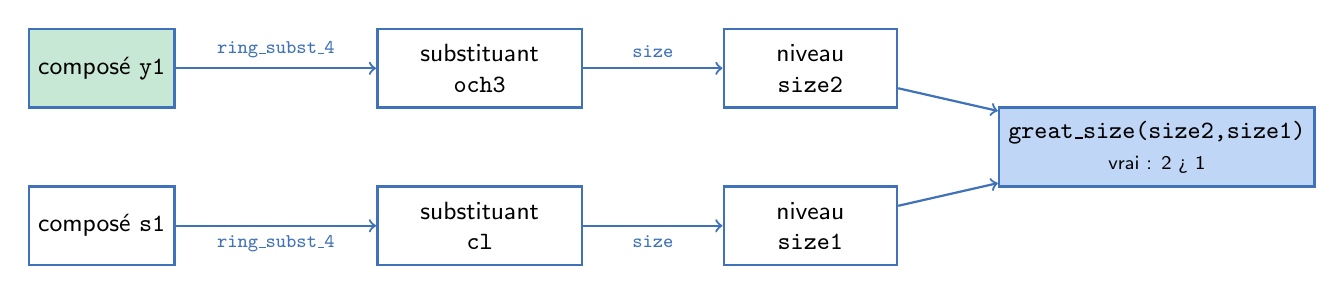
\begin{tikzpicture}[x=1cm,y=1cm, every node/.style={font=\small}, box/.style={draw=marine,fill=white,line width=0.9pt,align=center,minimum height=1.0cm}]
  \node[box,fill=vert!25,minimum width=1.8cm] (X) at (0,1.0) {composé \texttt{y1}};
  \node[box,minimum width=1.8cm] (Y) at (0,-1.0) {composé \texttt{s1}};
  \node[box,minimum width=2.6cm] (SX) at (4.8,1.0) {substituant\\\texttt{och3}};
  \node[box,minimum width=2.6cm] (SY) at (4.8,-1.0) {substituant\\\texttt{cl}};
  \node[box,minimum width=2.2cm] (LX) at (9.0,1.0) {niveau\\\texttt{size2}};
  \node[box,minimum width=2.2cm] (LY) at (9.0,-1.0) {niveau\\\texttt{size1}};
  \node[box,fill=pastel,minimum width=3.4cm] (G) at (13.4,0) {\texttt{great\_size(size2,size1)}\\\scriptsize vrai : 2 > 1};
  \draw[->,thick,marine] (X) -- node[above,font=\scriptsize\ttfamily]{ring\_subst\_4} (SX);
  \draw[->,thick,marine] (Y) -- node[below,font=\scriptsize\ttfamily]{ring\_subst\_4} (SY);
  \draw[->,thick,marine] (SX) -- node[above,font=\scriptsize\ttfamily]{size} (LX);
  \draw[->,thick,marine] (SY) -- node[below,font=\scriptsize\ttfamily]{size} (LY);
  \draw[->,thick,marine] (LX) -- (G);
  \draw[->,thick,marine] (LY) -- (G);
\end{tikzpicture}
\end{center}
\ce{lire de gauche à droite : composé $\to$ substituant $\to$ niveau $\to$ comparaison. Les propriétés (\texttt{polar}, \texttt{size}\ldots) sont attachées aux \emph{substituants}, pas aux composés : c'est pour cela qu'une règle sur \texttt{great(X,Y)} doit passer par \texttt{ring\_subst\_k}.}

\st{Une clause possible (illustration seulement)}
Voici la forme que peut prendre une règle qui suit cette chaîne :
\begin{moi}
\texttt{great(X,Y) :- ring\_subst\_4(X,A), ring\_subst\_4(Y,B), size(A,S), size(B,T), great\_size(S,T).}
\end{moi}
En français : \emph{\texttt{X} est meilleur que \texttt{Y} si le substituant de \texttt{X} en position 4 est plus gros que celui de \texttt{Y}.}
\textbf{Ce n'est pas la règle apprise.} Je l'ai testée : seuls 8 composés ont un substituant en position 4, la clause ne s'applique qu'à une petite minorité des paires (3 positifs et 1 négatif sur 530). Un vrai programme combine plusieurs clauses sur plusieurs positions et propriétés (\texttt{max\_clauses(6)}).
Les directions s'enchaînent comme dans les autres datasets : \texttt{ring\_subst\_4(in,out)} produit le substituant \texttt{A}, \texttt{size(in,out)} produit son niveau \texttt{S}, et \texttt{great\_size} compare deux niveaux déjà produits.

\titrebox{5}{Règles $\mathcal{R}$ et règle apprise}
\textbf{Règles $\mathcal{R}$ : aucune.} Le \texttt{bk.pl} (696 lignes) ne contient que des faits et deux directives \texttt{style\_check}. Il n'y a pas de règle à partager, donc $\mathcal{R}=\emptyset$.\par\vspace{3pt}
\textbf{Règle apprise :} aucun programme n'est documenté dans les fichiers, et je n'ai pas lancé Popper. Le biais autorise 31 prédicats dans le corps (propriétés, tables \texttt{great\_*}, \texttt{gt}\ldots), avec \texttt{max\_clauses(6)}, \texttt{max\_vars(5)} et \texttt{max\_body(6)} (7 pour \texttt{amine}, \texttt{mem} et \texttt{toxic}).

\titrebox{6}{Points de vigilance pour la preuve federated}
\begin{piege}
\textbf{Un exemple a deux constantes.} Dans Trains, un exemple \texttt{f(t800)} a une constante locale. Ici \texttt{great(X,Y)} en a \emph{deux}. L'énoncé de A1 (``pour tout $f(c)$, $c$ est locale au client $i$'') ne les couvre pas : la preuve doit être étendue à des exemples \emph{relationnels}, avec une garantie pour chacune des deux constantes.
\end{piege}
\begin{piege}
\textbf{La partition \texttt{iid\_3\_seed\_42} copie tout le BK.} J'ai ouvert le dossier : chaque client reçoit 628 faits et les 37 composés (les trois \texttt{bk.pl} sont identiques), seuls les exemples sont répartis (177, 177 et 176 de chaque classe). Donc $\mathcal{B}_i=\mathcal{B}$ : la Knowledge Locality est vraie trivialement, mais rien n'est privé. Même remarque que pour \texttt{iggp-rps}.
\end{piege}
\textbf{Directions :} déclarées. \texttt{great(in,in)} a ses deux arguments en entrée : la tête n'a pas de sortie, ce qui est cohérent avec une comparaison entre deux composés connus.

% =====================================================================
%  PART X : vue multi-relationnelle de tous les datasets
% =====================================================================
\partie{X}{La vue multi-relationnelle des datasets}{Pour chaque dataset : quelles relations, comment elles se relient, combien de lignes. Puis un tableau de comparaison et ce que cela change pour la preuve.}

\titrebox{1}{Ce que ``multi-relationnel'' veut dire}
\begin{itemize}
  \item Un prédicat Prolog (\texttt{has\_car/2}, \texttt{atm/5}\ldots) est une \EN{relation}{relation} : un tableau dont chaque fait est une \emph{ligne}.
  \item Un \EN{example}{exemple} n'est pas une ligne d'un seul tableau : c'est une \textbf{clé} (un train, un composé, un tour de jeu) autour de laquelle se trouvent des lignes dans \emph{plusieurs} relations, en nombre \emph{variable} (un train a 2, 3 ou 4 wagons).
  \item Les relations se relient par des constantes communes : une \EN{foreign key}{clé étrangère}. Dans \texttt{has\_car(t800,t800\_c1)} et \texttt{short(t800\_c1)}, la constante \texttt{t800\_c1} relie les deux tableaux.
  \item Une règle est une \EN{join}{jointure} : \texttt{f(A) :- has\_car(A,B), short(B).} veut dire ``prendre \texttt{has\_car}, la relier à \texttt{short} sur la colonne \texttt{B}''. En logique, on parle de \EN{conjunctive query}{requête conjonctive}.
\end{itemize}

\st{Pourquoi un seul tableau ne suffit pas (représentation propositionnelle)}
On peut essayer de ``mettre à plat'' Trains en une ligne par train, avec une colonne par propriété de wagon (\EN{attribute-value}{attribut-valeur}, ou \emph{propositionnel}) :
\renewcommand{\arraystretch}{1.25}
\begin{center}
\begin{tabular}{@{}l c l l l l@{}}
\textbf{train} & \textbf{\#wagons} & \textbf{wagon 1} & \textbf{wagon 2} & \textbf{wagon 3} & \textbf{wagon 4}\\\hline
\texttt{t800} & 4 & long, 2 roues, ouvert & long, 2 roues, fermé & long, 3 roues, ouvert & court, 2 roues, fermé\\
\texttt{t808} & 2 & long, 3 roues, fermé & long, 2 roues, ouvert & \textcolor{rouge}{(vide)} & \textcolor{rouge}{(vide)}\\
\end{tabular}
\end{center}
\begin{itemize}
  \item \textbf{Des cases vides} : le nombre de wagons change d'un train à l'autre, il faut fixer un maximum et remplir avec du vide. Pour un composé de Mutagenesis, il faudrait 40 colonnes d'atomes, et il n'y a plus de place pour les liaisons.
  \item \textbf{Un ordre artificiel} : les wagons n'ont pas d'ordre dans les données, mais le tableau en impose un. La règle ``un wagon à 3 roues et un autre wagon long à 2 roues'' devrait être écrite pour chaque couple de colonnes (4$\times$3 = 12 cas), au lieu d'une seule jointure.
  \item \textbf{Des liens perdus} : un chargement appartient à un wagon, qui appartient à un train. Le tableau plat ne garde pas cette chaîne, sauf à ajouter encore des colonnes.
\end{itemize}
\ce{l'\emph{aspect multi-relationnel} est ce qui rend l'ILP utile : une règle comme ``\texttt{has\_car(A,B), has\_car(A,C), long(C), three\_wheels(B), two\_wheels(C)}'' parle d'un \emph{nombre quelconque} de wagons sans avoir besoin d'en fixer un maximum.}

\st{Comment lire les schémas qui suivent}
Chaque boîte est une relation (ses colonnes sont listées). \colorbox{vert!25}{\strut vert} : relation à apprendre. Blanc : relation de données de l'exemple. \colorbox{pastel}{\strut bleu pâle} : relation \emph{partagée} (la même pour tous les exemples). \emph{Pointillé} : règle (relation calculée). Une flèche est une jointure sur la colonne indiquée ; ``1--N'' veut dire un-à-plusieurs.

\titrebox{2}{Trains : une chaîne train $\to$ wagon $\to$ chargement}
\begin{center}
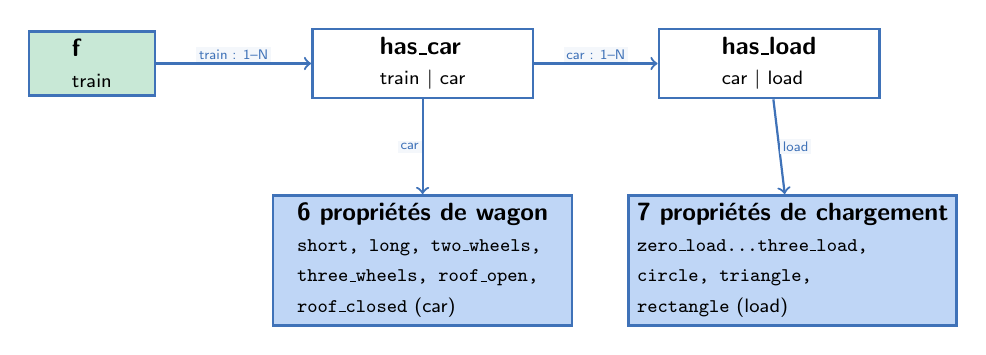
\begin{tikzpicture}[x=1cm,y=1cm]
\node[draw=marine,fill=vert!25,line width=0.9pt,minimum width=1.6cm,align=left,inner sep=3pt,font=\small] (f) at (0.00,0.00) {\textbf{f}\\ \scriptsize train};
\node[draw=marine,fill=white,line width=0.9pt,minimum width=2.8cm,align=left,inner sep=3pt,font=\small] (hc) at (4.20,0.00) {\textbf{has\_car}\\ \scriptsize train $\mid$ car};
\node[draw=marine,fill=white,line width=0.9pt,minimum width=2.8cm,align=left,inner sep=3pt,font=\small] (hl) at (8.60,0.00) {\textbf{has\_load}\\ \scriptsize car $\mid$ load};
\node[draw=marine,fill=pastel,line width=0.9pt,minimum width=3.8cm,align=left,inner sep=3pt,font=\small] (pc) at (4.20,-2.50) {\textbf{6 propriétés de wagon}\\ \scriptsize \texttt{short, long, two\_wheels,}\\ \scriptsize \texttt{three\_wheels, roof\_open,}\\ \scriptsize \texttt{roof\_closed}\ (car)};
\node[draw=marine,fill=pastel,line width=0.9pt,minimum width=3.8cm,align=left,inner sep=3pt,font=\small] (pl) at (8.90,-2.50) {\textbf{7 propriétés de chargement}\\ \scriptsize \texttt{zero\_load\ldots three\_load,}\\ \scriptsize \texttt{circle, triangle,}\\ \scriptsize \texttt{rectangle}\ (load)};
\draw[->,thick,marine] (f) -- node[above,font=\tiny,fill=fond,inner sep=1pt]{train : 1--N} (hc);
\draw[->,thick,marine] (hc) -- node[above,font=\tiny,fill=fond,inner sep=1pt]{car : 1--N} (hl);
\draw[->,thick,marine] (hc) -- node[left,font=\tiny,fill=fond,inner sep=1pt]{car} (pc);
\draw[->,thick,marine] (hl) -- node[right,font=\tiny,fill=fond,inner sep=1pt]{load} (pl);
\end{tikzpicture}
\end{center}
\textbf{Sur les 10 trains :} 32 lignes \texttt{has\_car} (de 2 à 4 wagons par train, 3,2 en moyenne), 41 lignes \texttt{has\_load}. 25 wagons sur 32 ont au moins un chargement (1 à 3), 7 n'en ont aucun.
\textbf{Profondeur de jointure :} 2 (train $\to$ wagon $\to$ chargement). \textbf{Clé :} \texttt{has\_load(car,load)} et les propriétés de wagon \emph{ne contiennent pas le train}. Le lien avec le train passe par \texttt{has\_car}, et par le nom des constantes (\texttt{t800\_c1}). \textbf{Dans la partition générée}, chaque client reçoit en plus les 990 trains sans exemple (28\,226 faits communs) : ils forment la partie partagée.

\titrebox{3}{Zendo : une structure, des pièces, des contacts}
\begin{center}
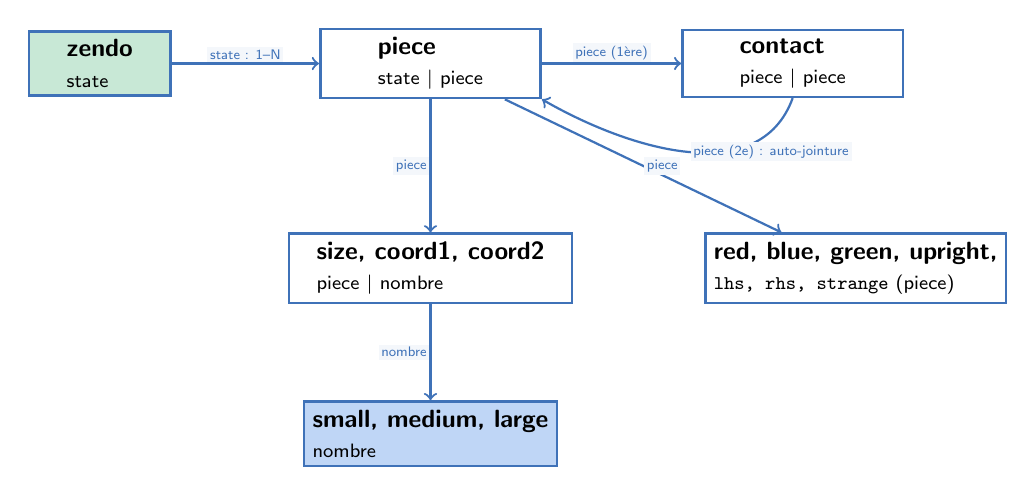
\begin{tikzpicture}[x=1cm,y=1cm]
\node[draw=marine,fill=vert!25,line width=0.9pt,minimum width=1.8cm,align=left,inner sep=3pt,font=\small] (z) at (0.00,0.00) {\textbf{zendo}\\ \scriptsize state};
\node[draw=marine,fill=white,line width=0.9pt,minimum width=2.8cm,align=left,inner sep=3pt,font=\small] (pi) at (4.20,0.00) {\textbf{piece}\\ \scriptsize state $\mid$ piece};
\node[draw=marine,fill=white,line width=0.9pt,minimum width=2.8cm,align=left,inner sep=3pt,font=\small] (co) at (8.80,0.00) {\textbf{contact}\\ \scriptsize piece $\mid$ piece};
\node[draw=marine,fill=white,line width=0.9pt,minimum width=3.6cm,align=left,inner sep=3pt,font=\small] (sz) at (4.20,-2.60) {\textbf{size, coord1, coord2}\\ \scriptsize piece $\mid$ nombre};
\node[draw=marine,fill=white,line width=0.9pt,minimum width=3.6cm,align=left,inner sep=3pt,font=\small] (cl) at (9.60,-2.60) {\textbf{red, blue, green, upright,}\\ \scriptsize \texttt{lhs, rhs, strange}\ (piece)};
\node[draw=marine,fill=pastel,line width=0.9pt,minimum width=3.0cm,align=left,inner sep=3pt,font=\small] (nb) at (4.20,-4.70) {\textbf{small, medium, large}\\ \scriptsize nombre};
\draw[->,thick,marine] (z) -- node[above,font=\tiny,fill=fond,inner sep=1pt]{state : 1--N} (pi);
\draw[->,thick,marine] (pi) -- node[above,font=\tiny,fill=fond,inner sep=1pt]{piece (1ère)} (co);
\draw[->,thick,marine] (co.south) to[out=-110,in=-30] node[right,font=\tiny,fill=fond,inner sep=1pt,xshift=1pt]{piece (2e) : auto-jointure} (pi.south east);
\draw[->,thick,marine] (pi) -- node[left,font=\tiny,fill=fond,inner sep=1pt]{piece} (sz);
\draw[->,thick,marine] (sz) -- node[left,font=\tiny,fill=fond,inner sep=1pt]{nombre} (nb);
\draw[->,thick,marine,bend left=10] (pi) -- node[right,font=\tiny,fill=fond,inner sep=1pt]{piece} (cl);
\end{tikzpicture}
\end{center}
\textbf{Sur les 40 structures :} 139 lignes \texttt{piece} (1 à 5 par structure), 139 lignes pour chacune de \texttt{size}, \texttt{coord1} et \texttt{coord2}, et 60 lignes \texttt{contact} distinctes (55 pièces touchent au moins une autre pièce, 1 ou 2 contacts chacune).
\textbf{Particularité :} \texttt{contact(piece,piece)} relie la relation \texttt{piece} \emph{à elle-même} : c'est une \EN{self-join}{auto-jointure}, ce qui donne un graphe. Les nombres (\texttt{size}) sont reliés à \texttt{small}/\texttt{medium}/\texttt{large}, une relation partagée.

\titrebox{4}{iggp-rps : tours, joueurs, scores}
\begin{center}
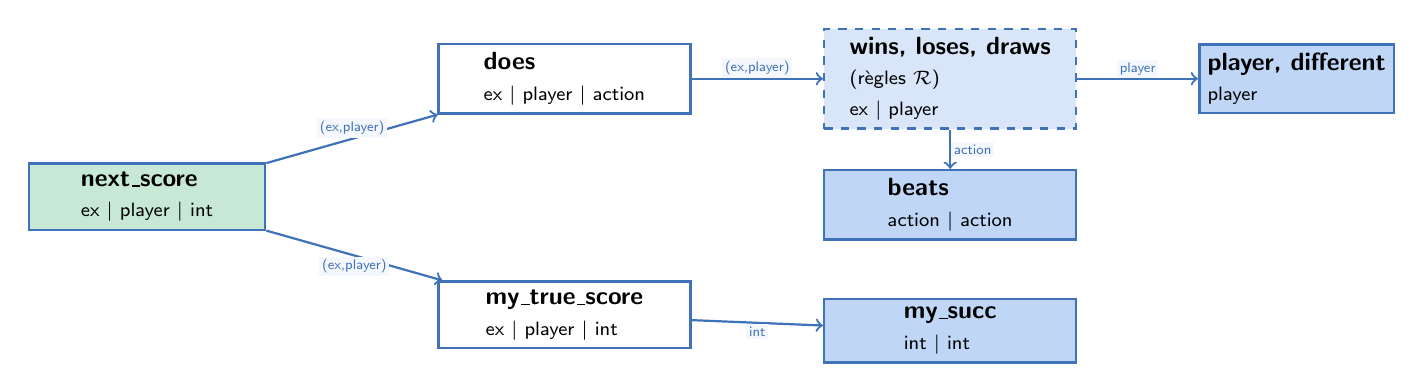
\begin{tikzpicture}[x=1cm,y=1cm]
\node[draw=marine,fill=vert!25,line width=0.9pt,minimum width=3.0cm,align=left,inner sep=3pt,font=\small] (ns) at (0.00,0.00) {\textbf{next\_score}\\ \scriptsize ex $\mid$ player $\mid$ int};
\node[draw=marine,fill=white,line width=0.9pt,minimum width=3.2cm,align=left,inner sep=3pt,font=\small] (do) at (5.30,1.50) {\textbf{does}\\ \scriptsize ex $\mid$ player $\mid$ action};
\node[draw=marine,fill=white,line width=0.9pt,minimum width=3.2cm,align=left,inner sep=3pt,font=\small] (ts) at (5.30,-1.50) {\textbf{my\_true\_score}\\ \scriptsize ex $\mid$ player $\mid$ int};
\node[draw=marine,fill=pastel!60,line width=0.9pt,dashed,minimum width=3.2cm,align=left,inner sep=3pt,font=\small] (ru) at (10.20,1.50) {\textbf{wins, loses, draws}\\ \scriptsize (règles $\mathcal{R}$)\\ \scriptsize ex $\mid$ player};
\node[draw=marine,fill=pastel,line width=0.9pt,minimum width=3.2cm,align=left,inner sep=3pt,font=\small] (be) at (10.20,-0.10) {\textbf{beats}\\ \scriptsize action $\mid$ action};
\node[draw=marine,fill=pastel,line width=0.9pt,minimum width=3.2cm,align=left,inner sep=3pt,font=\small] (su) at (10.20,-1.70) {\textbf{my\_succ}\\ \scriptsize int $\mid$ int};
\node[draw=marine,fill=pastel,line width=0.9pt,minimum width=2.4cm,align=left,inner sep=3pt,font=\small] (pl) at (14.60,1.50) {\textbf{player, different}\\ \scriptsize player};
\draw[->,thick,marine] (ns) -- node[above,font=\tiny,fill=fond,inner sep=1pt]{(ex,player)} (do);
\draw[->,thick,marine] (ns) -- node[below,font=\tiny,fill=fond,inner sep=1pt]{(ex,player)} (ts);
\draw[->,thick,marine] (do) -- node[above,font=\tiny,fill=fond,inner sep=1pt]{(ex,player)} (ru);
\draw[->,thick,marine] (ru) -- node[right,font=\tiny,fill=fond,inner sep=1pt]{action} (be);
\draw[->,thick,marine] (ts) -- node[below,font=\tiny,fill=fond,inner sep=1pt]{int} (su);
\draw[->,thick,marine] (ru) -- node[above,font=\tiny,fill=fond,inner sep=1pt]{player} (pl);
\end{tikzpicture}
\end{center}
\textbf{Sur les 58 tours :} 108 lignes \texttt{does} (2 par tour, pour 54 tours), 116 lignes \texttt{my\_true\_score} (2 par tour, 58 tours). La \emph{clé est composite} : (\texttt{ex}, \texttt{player}), et le but \texttt{next\_score} a 3 colonnes.
\textbf{Particularité :} la règle \texttt{wins} relie \texttt{does} à elle-même (\texttt{does(E,A,B), does(E,C,D)}), pour comparer les deux joueurs du même tour : auto-jointure sur \texttt{E}. Elle appelle ensuite \texttt{beats}, relation partagée.

\titrebox{5}{Mutagenesis : un graphe d'atomes par composé}
\begin{center}
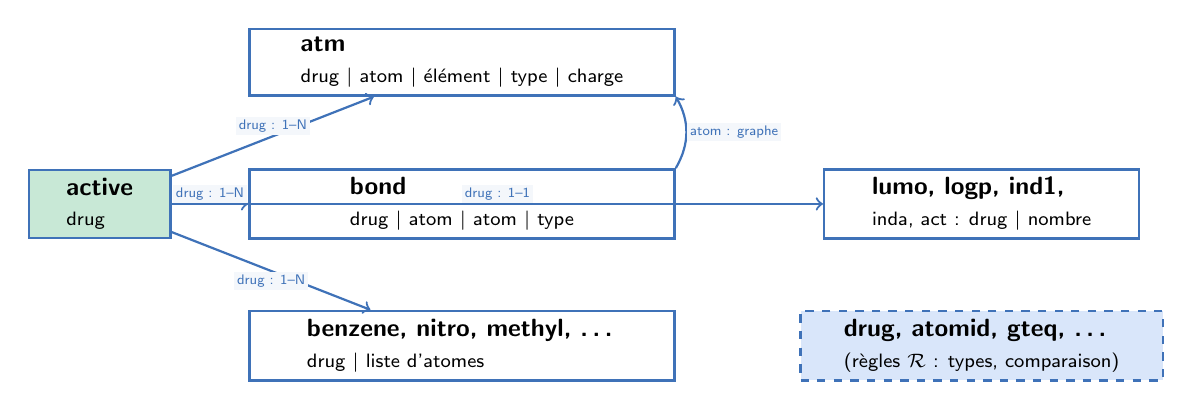
\begin{tikzpicture}[x=1cm,y=1cm]
\node[draw=marine,fill=vert!25,line width=0.9pt,minimum width=1.8cm,align=left,inner sep=3pt,font=\small] (a) at (0.00,0.00) {\textbf{active}\\ \scriptsize drug};
\node[draw=marine,fill=white,line width=0.9pt,minimum width=5.4cm,align=left,inner sep=3pt,font=\small] (at) at (4.60,1.80) {\textbf{atm}\\ \scriptsize drug $\mid$ atom $\mid$ élément $\mid$ type $\mid$ charge};
\node[draw=marine,fill=white,line width=0.9pt,minimum width=5.4cm,align=left,inner sep=3pt,font=\small] (bo) at (4.60,0.00) {\textbf{bond}\\ \scriptsize drug $\mid$ atom $\mid$ atom $\mid$ type};
\node[draw=marine,fill=white,line width=0.9pt,minimum width=5.4cm,align=left,inner sep=3pt,font=\small] (gr) at (4.60,-1.80) {\textbf{benzene, nitro, methyl, \ldots}\\ \scriptsize drug $\mid$ liste d'atomes};
\node[draw=marine,fill=white,line width=0.9pt,minimum width=4.0cm,align=left,inner sep=3pt,font=\small] (me) at (11.20,0.00) {\textbf{lumo, logp, ind1,}\\ \scriptsize inda, act : drug $\mid$ nombre};
\node[draw=marine,fill=pastel!60,line width=0.9pt,dashed,minimum width=4.6cm,align=left,inner sep=3pt,font=\small] (ty) at (11.20,-1.80) {\textbf{drug, atomid, gteq, \ldots}\\ \scriptsize (règles $\mathcal{R}$ : types, comparaison)};
\draw[->,thick,marine,bend left=15] (a) -- node[above,font=\tiny,fill=fond,inner sep=1pt]{drug : 1--N} (at);
\draw[->,thick,marine] (a) -- node[above,font=\tiny,fill=fond,inner sep=1pt]{drug : 1--N} (bo);
\draw[->,thick,marine,bend right=15] (a) -- node[below,font=\tiny,fill=fond,inner sep=1pt]{drug : 1--N} (gr);
\draw[->,thick,marine,out=20,in=160,looseness=0.6] (a) -- node[above,font=\tiny,fill=fond,inner sep=1pt]{drug : 1--1} (me);
\draw[->,thick,marine] (bo.north east) to[out=60,in=-60] node[right,font=\tiny,fill=fond,inner sep=1pt]{atom : graphe} (at.south east);
\end{tikzpicture}
\end{center}
\textbf{Sur les 230 composés :} 5894 lignes \texttt{atm} (13 à 40 par composé, 25,6 en moyenne), 6309 lignes \texttt{bond} (13 à 44), 1712 lignes de groupes chimiques (listes d'atomes), et 230 lignes pour chaque mesure (\texttt{lumo}, \texttt{logp}, \texttt{ind1}, \texttt{inda}, \texttt{act}).
\textbf{Particularité :} \texttt{bond} relie \texttt{atm} à elle-même (atome--atome) : chaque composé est un \textbf{graphe}. La profondeur de jointure n'est pas bornée (une chaîne de liaisons), elle est limitée par \texttt{max\_body(6)}. \textbf{Clé :} le composé est la \emph{première colonne} de \texttt{atm}, \texttt{bond} et des groupes : la clé est dans chaque relation.

\titrebox{6}{Carcinogenesis : le même schéma, plus de relations}
\begin{center}
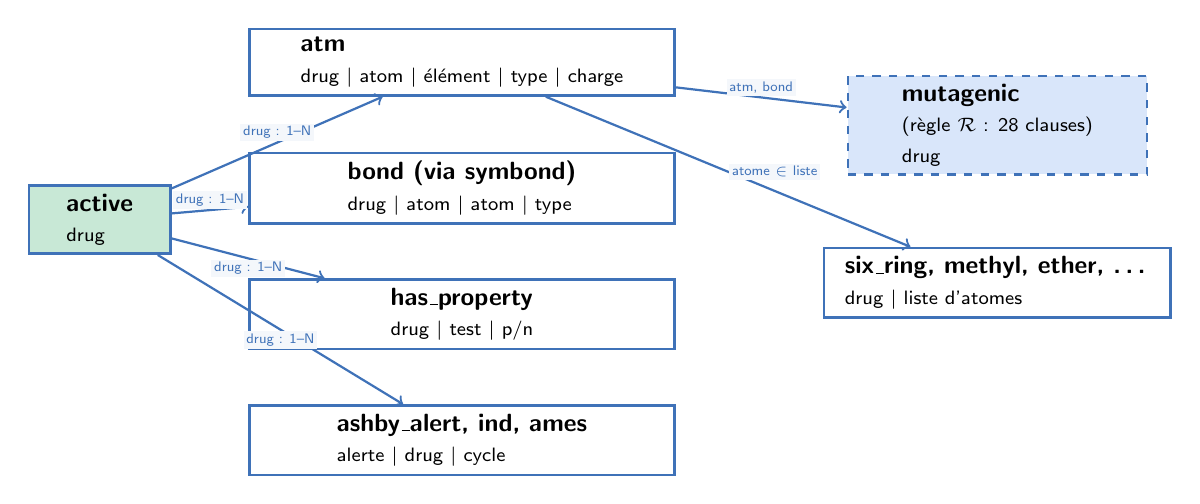
\begin{tikzpicture}[x=1cm,y=1cm]
\node[draw=marine,fill=vert!25,line width=0.9pt,minimum width=1.8cm,align=left,inner sep=3pt,font=\small] (a) at (0.00,0.20) {\textbf{active}\\ \scriptsize drug};
\node[draw=marine,fill=white,line width=0.9pt,minimum width=5.4cm,align=left,inner sep=3pt,font=\small] (at) at (4.60,2.20) {\textbf{atm}\\ \scriptsize drug $\mid$ atom $\mid$ élément $\mid$ type $\mid$ charge};
\node[draw=marine,fill=white,line width=0.9pt,minimum width=5.4cm,align=left,inner sep=3pt,font=\small] (bo) at (4.60,0.60) {\textbf{bond (via symbond)}\\ \scriptsize drug $\mid$ atom $\mid$ atom $\mid$ type};
\node[draw=marine,fill=white,line width=0.9pt,minimum width=5.4cm,align=left,inner sep=3pt,font=\small] (hp) at (4.60,-1.00) {\textbf{has\_property}\\ \scriptsize drug $\mid$ test $\mid$ p/n};
\node[draw=marine,fill=white,line width=0.9pt,minimum width=5.4cm,align=left,inner sep=3pt,font=\small] (al) at (4.60,-2.60) {\textbf{ashby\_alert, ind, ames}\\ \scriptsize alerte $\mid$ drug $\mid$ cycle};
\node[draw=marine,fill=pastel!60,line width=0.9pt,dashed,minimum width=3.8cm,align=left,inner sep=3pt,font=\small] (mu) at (11.40,1.40) {\textbf{mutagenic}\\ \scriptsize (règle $\mathcal{R}$ : 28 clauses)\\ \scriptsize drug};
\node[draw=marine,fill=white,line width=0.9pt,minimum width=4.4cm,align=left,inner sep=3pt,font=\small] (gr) at (11.40,-0.60) {\textbf{six\_ring, methyl, ether, \ldots}\\ \scriptsize drug $\mid$ liste d'atomes};
\draw[->,thick,marine,bend left=15] (a) -- node[above,font=\tiny,fill=fond,inner sep=1pt]{drug : 1--N} (at);
\draw[->,thick,marine] (a) -- node[above,font=\tiny,fill=fond,inner sep=1pt]{drug : 1--N} (bo);
\draw[->,thick,marine] (a) -- node[below,font=\tiny,fill=fond,inner sep=1pt]{drug : 1--N} (hp);
\draw[->,thick,marine,bend right=15] (a) -- node[below,font=\tiny,fill=fond,inner sep=1pt]{drug : 1--N} (al);
\draw[->,thick,marine] (at) -- node[above,font=\tiny,fill=fond,inner sep=1pt]{atm, bond} (mu);
\draw[->,thick,marine] (at) -- node[right,font=\tiny,fill=fond,inner sep=1pt]{atome $\in$ liste} (gr);
\end{tikzpicture}
\end{center}
\textbf{Chiffres :} 9205 lignes \texttt{atm} (1 à 214 atomes par composé, 26,5 en moyenne), 9319 \texttt{bond}, 1319 \texttt{has\_property} (jusqu'à 8 tests par composé), 748 \texttt{ashby\_alert}, 394 \texttt{ind}.
\textbf{Nouveauté :} \texttt{has\_property(drug,test,valeur)} est une relation \emph{à trois colonnes} : un composé a plusieurs lignes, une par test. \texttt{mutagenic(drug)} est une relation \emph{calculée} par 28 règles à partir de \texttt{atm} et \texttt{bond}.

\titrebox{7}{Alzheimer : deux composés comparés, via leurs substituants}
\begin{center}
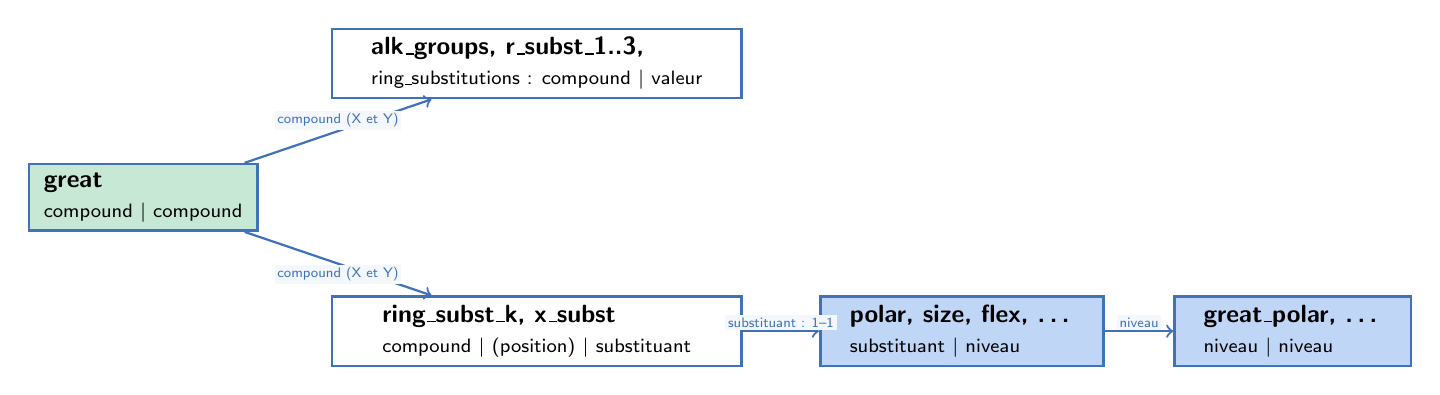
\begin{tikzpicture}[x=1cm,y=1cm]
\node[draw=marine,fill=vert!25,line width=0.9pt,minimum width=2.9cm,align=left,inner sep=3pt,font=\small] (g) at (0.00,0.00) {\textbf{great}\\ \scriptsize compound $\mid$ compound};
\node[draw=marine,fill=white,line width=0.9pt,minimum width=5.2cm,align=left,inner sep=3pt,font=\small] (cf) at (5.00,1.70) {\textbf{alk\_groups, r\_subst\_1..3,}\\ \scriptsize ring\_substitutions : compound $\mid$ valeur};
\node[draw=marine,fill=white,line width=0.9pt,minimum width=5.2cm,align=left,inner sep=3pt,font=\small] (rs) at (5.00,-1.70) {\textbf{ring\_subst\_k, x\_subst}\\ \scriptsize compound $\mid$ (position) $\mid$ substituant};
\node[draw=marine,fill=pastel,line width=0.9pt,minimum width=3.6cm,align=left,inner sep=3pt,font=\small] (pr) at (10.40,-1.70) {\textbf{polar, size, flex, \ldots}\\ \scriptsize substituant $\mid$ niveau};
\node[draw=marine,fill=pastel,line width=0.9pt,minimum width=3.0cm,align=left,inner sep=3pt,font=\small] (gp) at (14.60,-1.70) {\textbf{great\_polar, \ldots}\\ \scriptsize niveau $\mid$ niveau};
\draw[->,thick,marine] (g) -- node[above,font=\tiny,fill=fond,inner sep=1pt]{compound (X et Y)} (cf);
\draw[->,thick,marine] (g) -- node[below,font=\tiny,fill=fond,inner sep=1pt]{compound (X et Y)} (rs);
\draw[->,thick,marine] (rs) -- node[above,font=\tiny,fill=fond,inner sep=1pt]{substituant : 1--1} (pr);
\draw[->,thick,marine] (pr) -- node[above,font=\tiny,fill=fond,inner sep=1pt]{niveau} (gp);
\end{tikzpicture}
\end{center}
\textbf{Chiffres :} 37 composés ; 34 lignes de substituants pour 28 composés (0 à 5 par composé) ; 5 substituants décrits par 9 propriétés ; 9 relations de comparaison de 45 lignes. Le but \texttt{great(X,Y)} a \textbf{deux colonnes de type composé} : sur \texttt{acetyl}, chaque composé apparaît 24 à 33 fois en première position et 23 à 32 fois en seconde.
\textbf{Particularité :} la jointure forme un \emph{losange} : X et Y descendent chacun jusqu'à un substituant, puis un niveau, et se retrouvent dans la table de comparaison \texttt{great\_*}. Les relations de droite sont partagées entre tous les exemples.

\titrebox{8}{Comparaison des six datasets}
\renewcommand{\arraystretch}{1.3}
{\footnotesize
\begin{tabular}{@{}L{1.9cm}L{2.2cm}L{3.1cm}L{2.9cm}L{2.2cm}L{3.8cm}@{}}
\textbf{Dataset} & \textbf{Clé de l'exemple} & \textbf{Relations (arité $\ge2$)} & \textbf{Un-à-plusieurs} & \textbf{Auto-jointure / graphe} & \textbf{Clé dans chaque relation ?}\\\hline
Trains & \texttt{train} & \texttt{has\_car}, \texttt{has\_load} & 2--4 wagons, 0--3 chargements & non & \textbf{non} (via \texttt{has\_car}, nom \texttt{t800\_c1})\\
Zendo & \texttt{state} & \texttt{piece}, \texttt{contact}, \texttt{size}, \texttt{coord1}, \texttt{coord2} & 1--5 pièces & oui (\texttt{contact}) & \textbf{non} (\texttt{size}, \texttt{contact} ne portent pas l'état)\\
iggp-rps & (\texttt{ex}, \texttt{player}) & \texttt{does}, \texttt{my\_true\_score}, \texttt{beats}, \texttt{my\_succ} & 2 joueurs par tour & oui (\texttt{does} $\times$ \texttt{does}) & oui (\texttt{ex} en 1\textsuperscript{re} colonne)\\
Mutagenesis & \texttt{drug} & \texttt{atm}, \texttt{bond}, 12 groupes & 13--40 atomes & oui (\texttt{bond}) & oui (\texttt{drug} en 1\textsuperscript{re} colonne)\\
Carcinogenesis & \texttt{drug} & \texttt{atm}, \texttt{bond}, \texttt{has\_property}, \texttt{ashby\_alert}, \texttt{ind} & 1--214 atomes, $\le$ 8 tests & oui (\texttt{bond}) & oui\\
Alzheimer & paire (\texttt{compound}, \texttt{compound}) & \texttt{ring\_subst\_k}, \texttt{x\_subst}, propriétés, \texttt{great\_*} & 0--5 substituants & non (mais jointure en losange) & oui pour les faits par composé ; tables de niveaux \textbf{partagées}\\
\end{tabular}}

\vspace{4pt}
\renewcommand{\arraystretch}{1.3}
{\footnotesize
\begin{tabular}{@{}L{1.9cm}L{14.5cm}@{}}
\textbf{Dataset} & \textbf{Ce qui est partagé par tous les clients ($\mathcal{R}$ et tables communes)}\\\hline
Trains & les faits de 990 trains sans exemple (28\,226 faits, identiques chez les trois clients), pas de règle\\
Zendo & \texttt{small}, \texttt{medium}, \texttt{large} (tranches de nombres)\\
iggp-rps & \texttt{beats}, \texttt{my\_succ}, \texttt{player}, \texttt{different} et les 3 règles \texttt{wins}, \texttt{loses}, \texttt{draws}\\
Mutagenesis & 12 règles utilitaires (types, \texttt{append}, \texttt{gteq}, \texttt{lteq})\\
Carcinogenesis & environ 46 règles, dont les 28 clauses \texttt{mutagenic/1}\\
Alzheimer & presque tout : propriétés des substituants, tables \texttt{great\_*}, \texttt{gt}\\
\end{tabular}}

\titrebox{9}{Ce que cela change pour la preuve federated}
\st{Deux formes de schéma : en étoile ou en chaîne}
\begin{itemize}
  \item \textbf{En étoile} (iggp-rps, Mutagenesis, Carcinogenesis, faits par composé d'Alzheimer) : la \textbf{clé de l'exemple est la première colonne de chaque relation}. Partager les données entre clients revient à filtrer sur cette colonne. Les littéraux restent liés à l'exemple dès qu'ils sont appelés avec la clé (garde ``une seule variable de type \texttt{drug}'').
  \item \textbf{En chaîne} (Trains, Zendo) : seule la première relation (\texttt{has\_car}, \texttt{piece}) porte la clé ; les suivantes (\texttt{has\_load}, \texttt{size}, \texttt{contact}\ldots) ne la portent pas. Une ligne de \texttt{has\_load} n'appartient à un train que parce que la constante \texttt{t800\_c1} \emph{a été produite par} \texttt{has\_car(t800,\ldots)}. Il faut donc \textbf{suivre la chaîne} : c'est exactement le rôle de l'\emph{invariant} (``constantes autorisées'') et des \emph{directions} dans la preuve de la Knowledge Locality.
\end{itemize}
\st{Où chaque hypothèse intervient}
\renewcommand{\arraystretch}{1.3}
\begin{tabular}{@{}L{3.2cm}L{13.2cm}@{}}
\textbf{Assumption} & \textbf{Lien avec le schéma relationnel}\\\hline
A1 Example Locality & la clé de l'exemple (train, composé, tour) est une constante locale ; pour Alzheimer, un exemple a \emph{deux} clés (X et Y)\\
A2 Separated Local Constants & les clés étrangères (\texttt{t800\_c1}, \texttt{d12\_3}, \texttt{p0\_2}) sont préfixées par la clé de l'exemple, donc deux clients ne partagent aucune ligne de données ; les relations \emph{partagées} (bleu pâle) ne doivent contenir aucune constante locale\\
A3 Directions & une jointure ne peut partir que de ce qui a déjà été produit : \texttt{has\_car(in,out)} produit le wagon, \texttt{short(in)} le lit. C'est ce qui interdit une jointure ``libre'' qui irait chercher des lignes d'un autre client\\
\end{tabular}
\ce{multi-relationnel signifie ``plusieurs tableaux reliés par des clés''. La preuve de la Knowledge Locality dit : tant que chaque jointure part de la clé de l'exemple et suit les clés produites, toutes les lignes utilisées sont chez le client qui détient l'exemple.}

\end{document}
